\part{Unterstützung} % (fold)
\label{prt:umsetzung}

\section*{Einleitung} % (fold)
\label{sec:umsetzung_einleitung}
\thispagestyle{empty}

Basierend auf den diese Arbeit motivierenden Grundlagen, die in den letzten Kapiteln beschrieben wurden, wird in diesem Teil auf die konkreten Maßnahmen zur Unterstützung von Articulation Work eingegangen. Ziel dieses Teils ist es, sowohl das hier vorgeschlagene Vorgehen bei der Unterstützung expliziter Articulation Work als auch die Unterstützung, die ein Werkzeug dabei leisten kann, umfassend dazustellen.

Auf Grundlage der Methodik, die im Kontext von Concept Mapping und Strukturlegetechniken vorgeschlagen wird und unter Berücksichtigung der Anforderungen, die aus dem inhärent kollaborativen Anwendungsszenario abgeleitet werden können, muss das Vorgehen zur Durchführung von expliziter Articulation Work festgelegt werden. 

In Rahmen der Festlegung des Vorgehens werden auch jene Aspekte identifiziert, in denen Unterstützung durch technische Werkzeuge sinnvoll und notwendig ist. Die Anforderungen, die sich aus diesen Aspekten ableiten lassen, bilden die Grundlage für die Konzeption und Umsetzung eines Werkzeugs, das diese Unterstützung bietet. Die technischen Details der Implementierung dieses Werkzeugs und die zugrunde liegenden konzeptionellen und technologischen Grundlagen bilden den Kern dieser Arbeit.

Der Aufbau dieses Teils folgt dem eben umrissenen inhaltlichen Vorgehen. In Kapitel \ref{cha:methodik} wird die Methodik zur Unterstützung expliziter Artikulation Work beschrieben. Aus diesem werden im darauf folgenden Kapitel \ref{cha:anforderungen} jene Bereiche identifiziert, in denen eine technologische Unterstützung notwendig ist und die Anforderungen an ein Werkzeug abgeleitet, das diese Unterstützung bietet. Die vier folgenden Kapitel beschäftigen sich mit der Umsetzung des Werkzeugs. Kapitel \ref{cha:implementierung_Überblick} beschäftigt sich dabei mit den konzeptionellen Grundlagen des Forschungsgebiets "Tangible Interfaces", das die Basis für die technische Umsetzung bildet. Kapitel \ref{cha:input_&_interpretation} beschäftigt sich mit jenen Technologien und Softwarekomponenten, die für die Informationseingabe in das technische System verwendet werden. Dabei wird auch auf die konkrete Interaktion der Benutzer mit dem System eingegangen. Kapitel \ref{cha:visualisierung} beschreibt die Ausgabeseite des technischen Systems und behandelt die Umsetzung des Informationsflusses vom System zu den Benutzern. Letztendlich wird in Kapitel \ref{cha:persistierung} beschrieben, welche Maßnahmen zu Sicherung der Ergebnisse der expliziten Articulation Work getroffen werden müssen und welche Möglichkeiten der technischen Umsetzung bestehen bzw. gewählt wurden.

% section umsetzung_einleitung (end)

\chapter{Methodik und Anwendungszenarien} % (fold)
\label{cha:methodik}

In diesem Kapitel wird die Methodik vorgestellt, die zur Externalisierung von mentalen Modellen mit dem zu entwickelnden Werkzeug zur Anwendung kommt. Die Inhalte dieses Kapitels bauen auf den Ergebnissen der Kapitel \ref{cha:articulation_work}  und \ref{cha:mentale_modelle} auf. Die Anforderungen, die sich auf der hier vorgestellen Methodik ergeben, werden in Kapitel \ref{cha:anforderungen} identifiziert und in weiterer Folge in einem Werkzeug umgesetzt.

Basierend auf den Schlussfolgerungen, die \citet{Ifenthaler06} hinsichtlich der Eignung der beschriebenen Methoden zur Externalisierung von mentalen Modellen zieht, scheinen jene Ansätze, die auf der Bildung diagrammatischer Modelle basieren besser für die Unterstützung expliziter „Articulation Work“ geeignet zu sein als Methoden, die auf einer rein natürlichsprachlichen Repräsentation aufbauen. Dies liegt vor allem in der höheren Abstraktion begründet, die die externe Repräsentation als interindividuellen Ankerpunkt für Kommunikation besser geeignet macht. Dies deckt sich mit den Aussagen von  \citet{Sarini02}, \citet{Herrmann02}, \citet{Raposo04} oder \citet{Jorgensen04}, die aus Sicht von „Articulation Work“ für die Verwendung von (diagrammatischen) Modellen zur Unterstützung argumentieren.

Betrachtet man nun die beiden Vertreter der auf diagrammatischen Modellen aufbauenden Methoden -- Strukturlegetechniken und Concept Mapping --, so zeigt sich hinsichtlich der Eignung zum Unterstützung von „Articulation Work“ kein eindeutiger Vorteil für eine der beiden Methoden. Vielmehr weisen beide in diesem Kontext Vor- und Nachteile auf. Hier wird deshalb versucht, die Vorteile von Strukturlegetechniken -- im Wesentlichen die Unmittelbarkeit der physischen Repräsentation -- mit jenen von Concept Mapping -- der Flexibilität der Modellierung sowie der Möglichkeit der Unterstützung des Modellierungsprozesses durch Computersysteme -- zu vereinen.

Dabei wird auf das für „Articulation Work“ besser geeignete methodische Vorgehen von „Concept Mapping“ zurückgegriffen, während die Modellierungsumgebung an das Setting von „Strukturlegetechniken“ angepasst wird.

\section{Durchführungsrahmen} % (fold)
\label{sec:durchführungsrahmen}

Der Rahmen, in explizite „Articulation Work“ mit Unterstützung von externalisierten Modellen durchgeführt wird, ist an den Aufbau von Strukturlegetechniken angelehnt. Eine wesentliche Eigenschaft ist hierbei die physische Modellierungsoberfläche, auf der das Modell mittels real vorhandener und unmittelbar manipulierbaren Elementen aufgebaut wird. 

Im Sinne der Abstimmung unterschiedlicher Sichten muss eine kooperative, nicht exklusive Manipulierbarkeit des Modells gewährleistet sein. Das Modell selbst ist -- orientiert an der Offenheit der Repräsentation bei „Concept Mapping“ -- weder in der Art der Elemente noch der Beziehungen eingeschränkt. 

Hinsichtlich des Durchführungsrahmen ist auch die Notwendigkeit des Einsatzes einer Person zu diskutieren, die den Externalisierungsprozess anleitet und steuernd in diesen eingreift. Die Dialog-Konsens-Methode, die im Rahmen von Strukturlegetechniken zur Anwendung kommt, sieht die Rolle eines Untersuchungsleiters vor, der den Ablauf der Externalisierung strukturell anleitet. Inhaltlich hat der Untersuchungsleiter jedoch keine neutrale Rolle inne, sondern tritt im Rahmen des Dialog-Konsens-Prozesses in Interaktion mit der externalisierenden Person. Ziel des Untersuchungsleiters ist es, das mentale Modell der externalisierenden Person zu erschließen und zu verstehen. In kooperativen Situationen (die von der Dialog-Konsens-Methode nach \citep{Scheele88} nicht explizit berücksichtigt werden), wo gegenseitiges Verständnis erreicht werden muss, wechselt demnach die Rolle des Untersuchungsleiters inhaltlich gesehen dynamisch. 

Aus Sicht der Prozesssteuerung kann zu diesem Zeitpunkt nicht entschieden werden, ob ein Untersuchungsleiter benötigt wird oder nicht. Bei Strukturlegetechniken beschränkt sich dessen Aufgabe auf die Sicherstellung der Fokussierung der beteiligten Personen auf die jeweilige Aufgabe. Im Rahmen der Concept Mapping Methode ist ein intervenierender Untersuchungsleiter nicht vorgesehen. Im Rahmen der empirischen Erhebung (siehe Kapitel XY) wird untersucht, ob diese Rolle bei der Anwendung des hier vorgeschlagenen Werkzeugs notwendig ist oder unbesetzt bleiben kann. 

% subsection durchführungsrahmen (end)

\section{Vorgehen} % (fold)
\label{sub:vorgehen}

Sowohl im Bereich der Strukturlegetechniken als auch im „Concept Mapping“ wird vorgeschlagen, den initialen Modellierungsprozess in zwei Phasen -- Konzeptsammlung und Konzeptstrukturierung -- zu teilen und in der Folge das Modell iterativ solange zu verändern bzw. zu erweitern, bis alle Beteiligten mit der Lösung zufrieden sind (im Bereich der Strukturlegetechniken wird die als „Dialog-Konsens“ bezeichnet, im „Concept Mapping“ spricht man von „Revisions“ des Modells, die erstellt werden müssen). Beide Abläufe sind abstrahiert in Abbildung \ref{fig:img_MentaleModelle_slt_cm} dargestellt.

\begin{figure}[htbp]
	\centering
		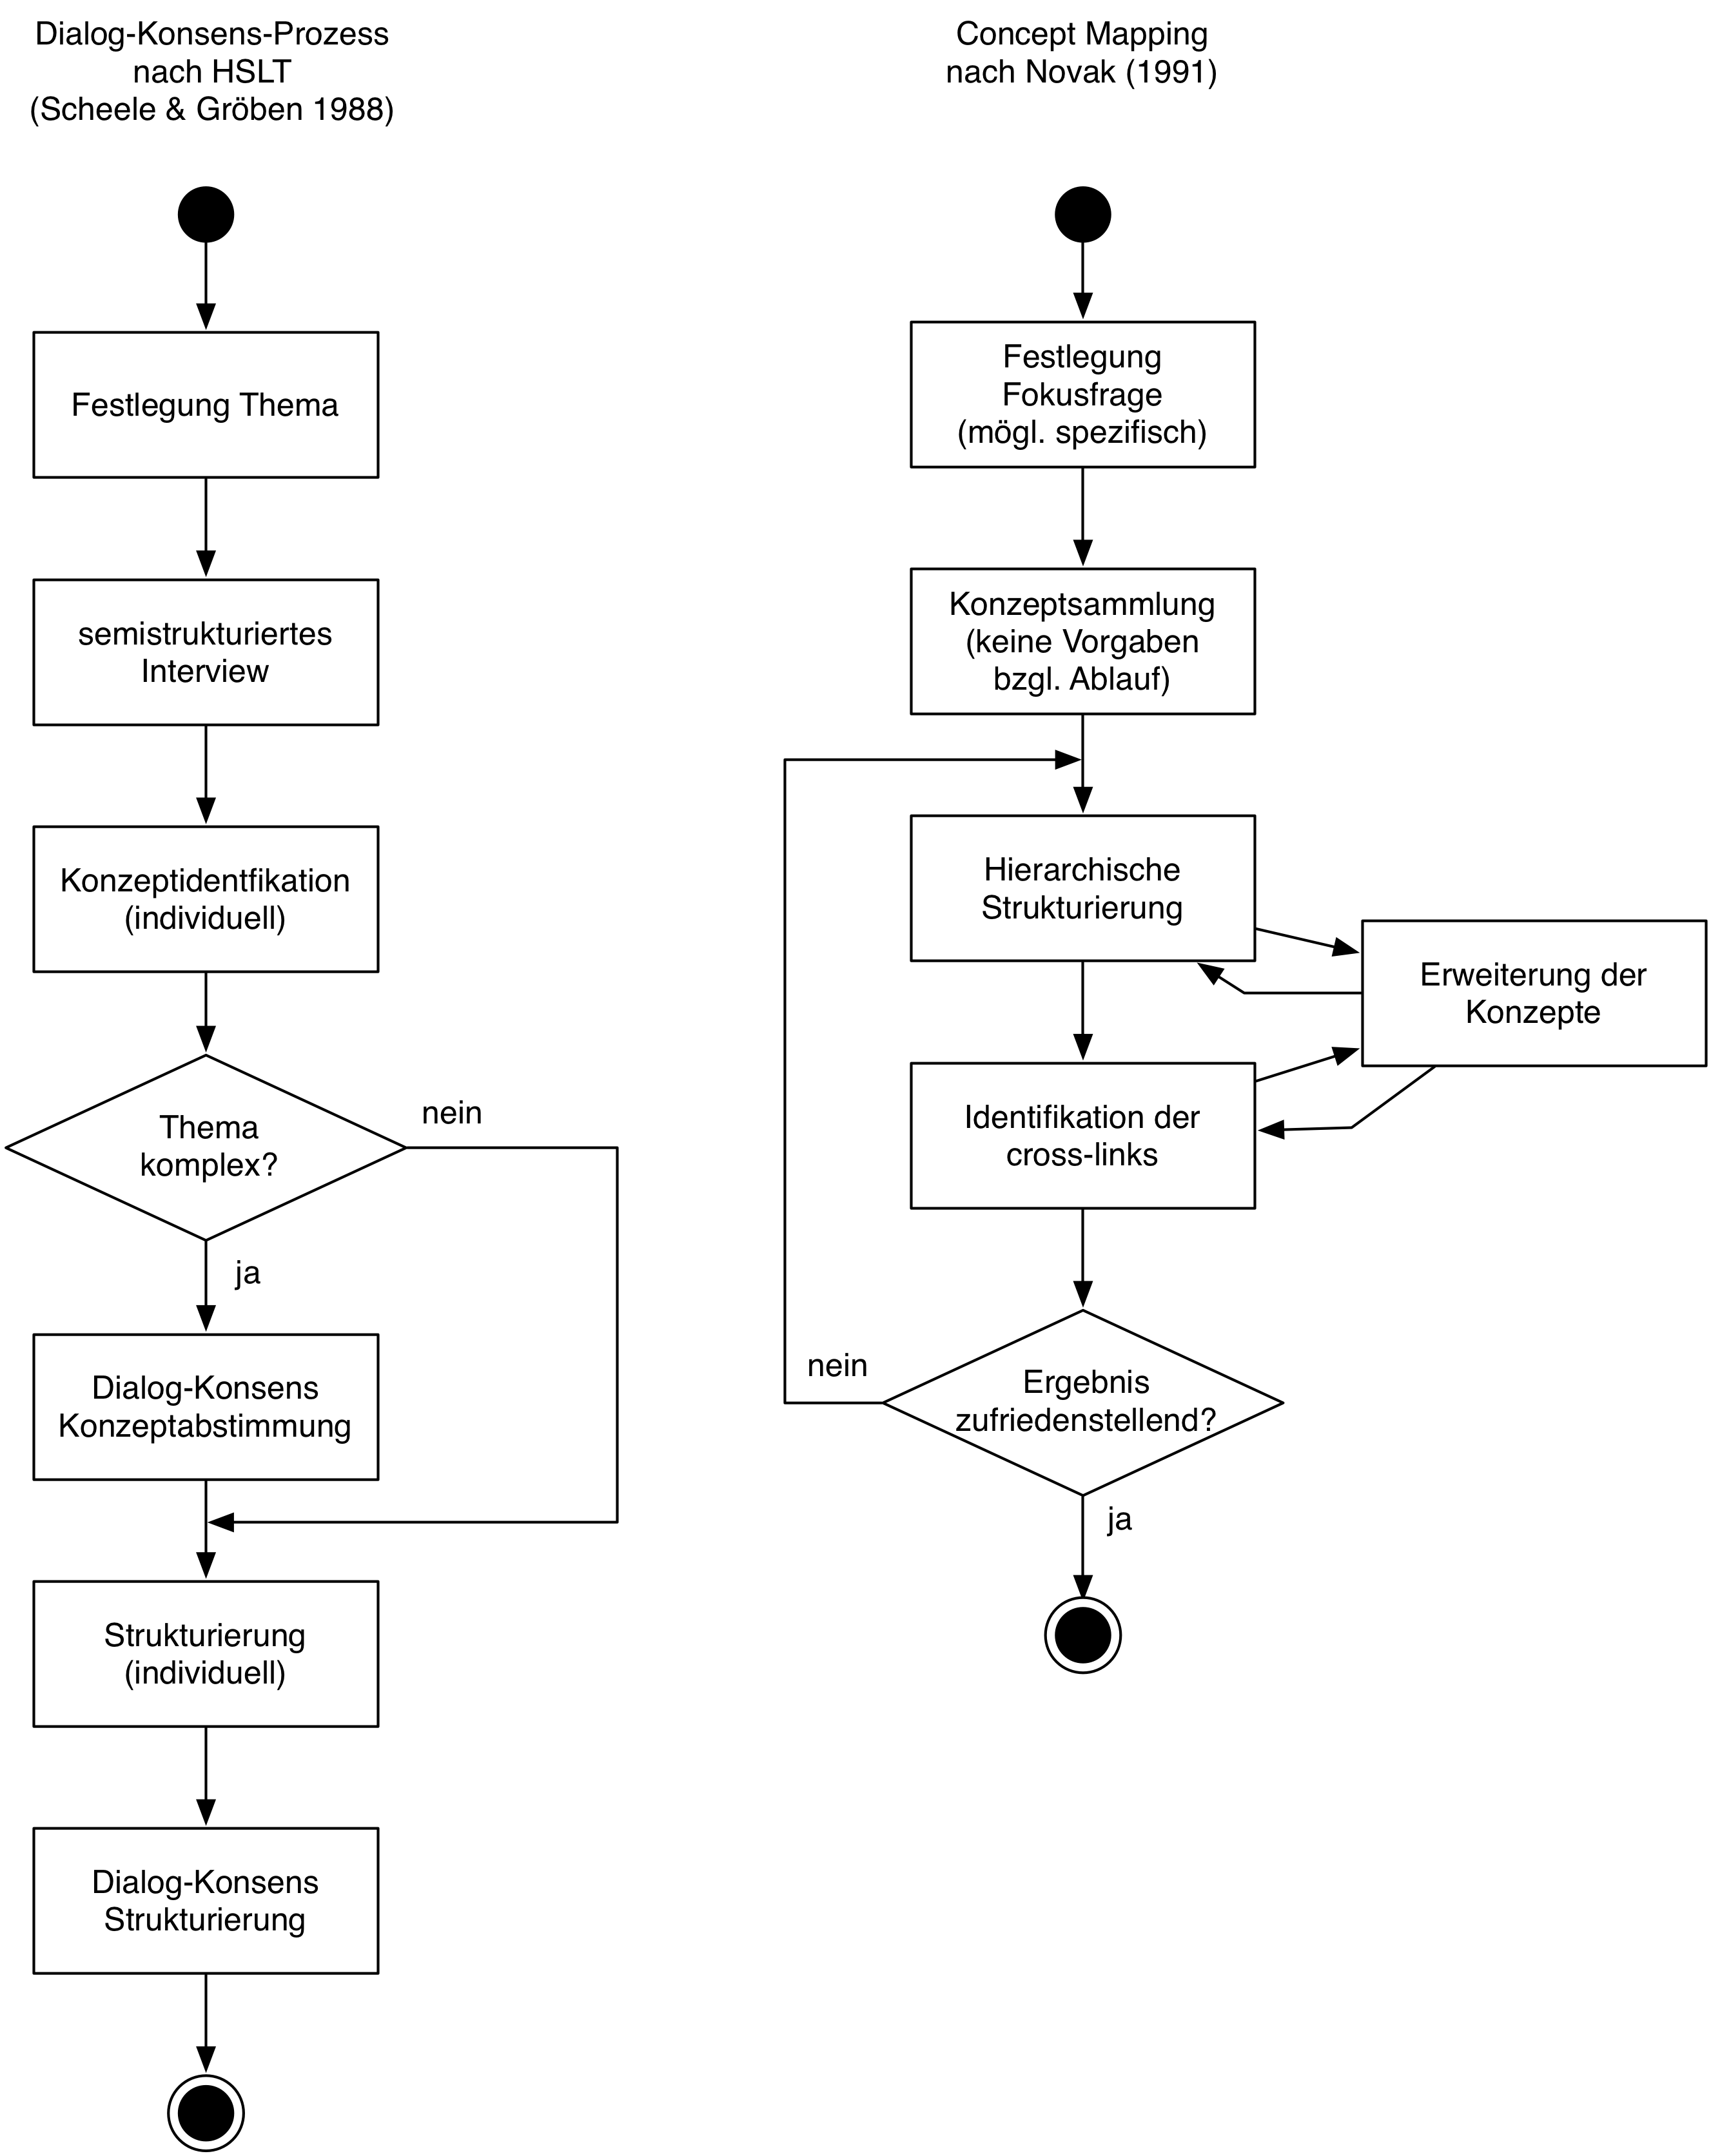
\includegraphics[width=\textwidth]{img/MentaleModelle/slt_cm.png}
	\caption{Externalisierung mentaler Modelle mittels Strukturlegetechniken und Concept Mapping}
	\label{fig:img_MentaleModelle_slt_cm}
\end{figure}

Das „Dialog-Konsens“-Vorgehen nach \citet{Scheele88} ist stark reglementiert und in den einzelnen Schritten mit definierten Methoden bzw. Vorgehensvorschriften hinterlegt. Die im Rahmen von „Concept Mapping“ vorgeschlagene Methode ist hier offener und erscheint damit für die Anwendung im Rahmen von „expliziter Articulation Work“ besser geeignet. Dies liegt am eher informellen Durchführungsrahmen von „expliziter Articulation Work“ begründet, deren Ausgestaltung individuell verschieden ist und zwischen den Beteiligten (im gängigsten Fall implizit) ausgehandelt wird. Ziel ist hier, den Artikulations-Prozess zu unterstützen und nicht, ihn zu formalisieren und in vorgegebene Ablauf-Grenzen zu pressen. 

Auch die zweiphasige Durchführung des Modellierungsprozesses muss unter diesem Gesichtspunkt hinterfragt werden. Die Unterteilung in zwei Phasen erscheint bei der Beschreibung von konzeptionellen Modellen sinnvoll. Begründet liegt dies in der Vielfalt möglicher Strukturierierungsvarianten bei dieser Art von Modellen. Im Gegensatz dazu ist die zweistufige Abhandlung der Externalisierung bei Modellen von Abläufen nur bedingt sinnvoll, da Aktivitäts-Konzepte im Normalfall bereits in deren kausalen Abfolge externalisiert und dann bzw. parallel mit zusätzlichen Konzepten hinterlegt werden. Diese Form von Modellen ist bei der Abstimmung von Arbeit gängig, wird aber weder bei Concept Mapping noch bei Strukturlegetechniken explizit angesprochen. Insofern ist die explizite Durchführung der ersten Phase -- also der Konzeptsammung -- als optional anzusehen. Im Sinne der Methode zur Erstellung von Concept Maps nach /citep{Novak06} werden Konzeptsammlungs-Phasen in den iterativen Modellverfeinerungsprozess eingeflochten, wenn dies in der Situation als notwendig erscheint.

Die einzelnen Schritte, die bei der Anwendung des Werkzeugs zur Anwendung kommen, sind im Einzelnen:
\begin{itemize}
 \item Einschulung
 \item Konzeptsammlung 
 \item Konzeptstrukturierung
 \item Restrukturierung
\end{itemize}

Diese Aufzählung gibt keine Reihenfolge der durchzuführenden Schritte vor. Vielmehr sind die einzelnen Blöcke als Module zu sehen, die je nach Anwendungsfall zu einem beliebigen Zeitpunkt im Externalisierungsprozess (auch mehrfach) zur Anwendung kommen oder auch entfallen können. Im Folgenden wird die Durchführung der einzelnen Schritte kurz umrissen und angegeben, in welchen Situationen deren Einsatz angemessen bzw. notwendig erscheint.

\subsection{Einschulung}

\subsection{Konzeptsammlung}

\subsection{Konzeptstrukturierung}

\subsection{Restrukturierung}
% section vorgehen (end)

\section{Anwendungsszenarien}

Prototypische Zusammenstellungen der Vorgehensblöcke je nach Setting der Abstimmung mentaler Modelle.

\begin{itemize}
 \item Verfeinerung individueller mentaler Modelle (rein indiv.)
 \item Wissenstransfer (1:n)
 \item Abstimmung individueller mentaler Modelle (indiv -> koop.)
 \item Aushandlung individueller mentaler Modelle (von Beginn an koop.)
\end{itemize}




% chapter methodik (end)
\chapter{Anforderungen an ein Werkzeug} % (fold)
\label{cha:anforderungen}

Dieses Kapitel dient der Überleitung von den bislang auf konzeptioneller Ebene beschriebenen Überlegungen hin zur tatsächlichen Umsetzung der Werkzeugunterstützung für „Articulation Work“ mittels mentaler Modelle. Basierend auf den Erkenntnissen aus den Kapiteln \ref{cha:articulation_work} und \ref{cha:mentale_modelle} sowie der in Kapitel \ref{cha:methodik} entwickelten Methodik werden hier die funktionalen Anforderungen an das Werkzeug beschrieben.

\begin{figure}[htbp]
	\centering
		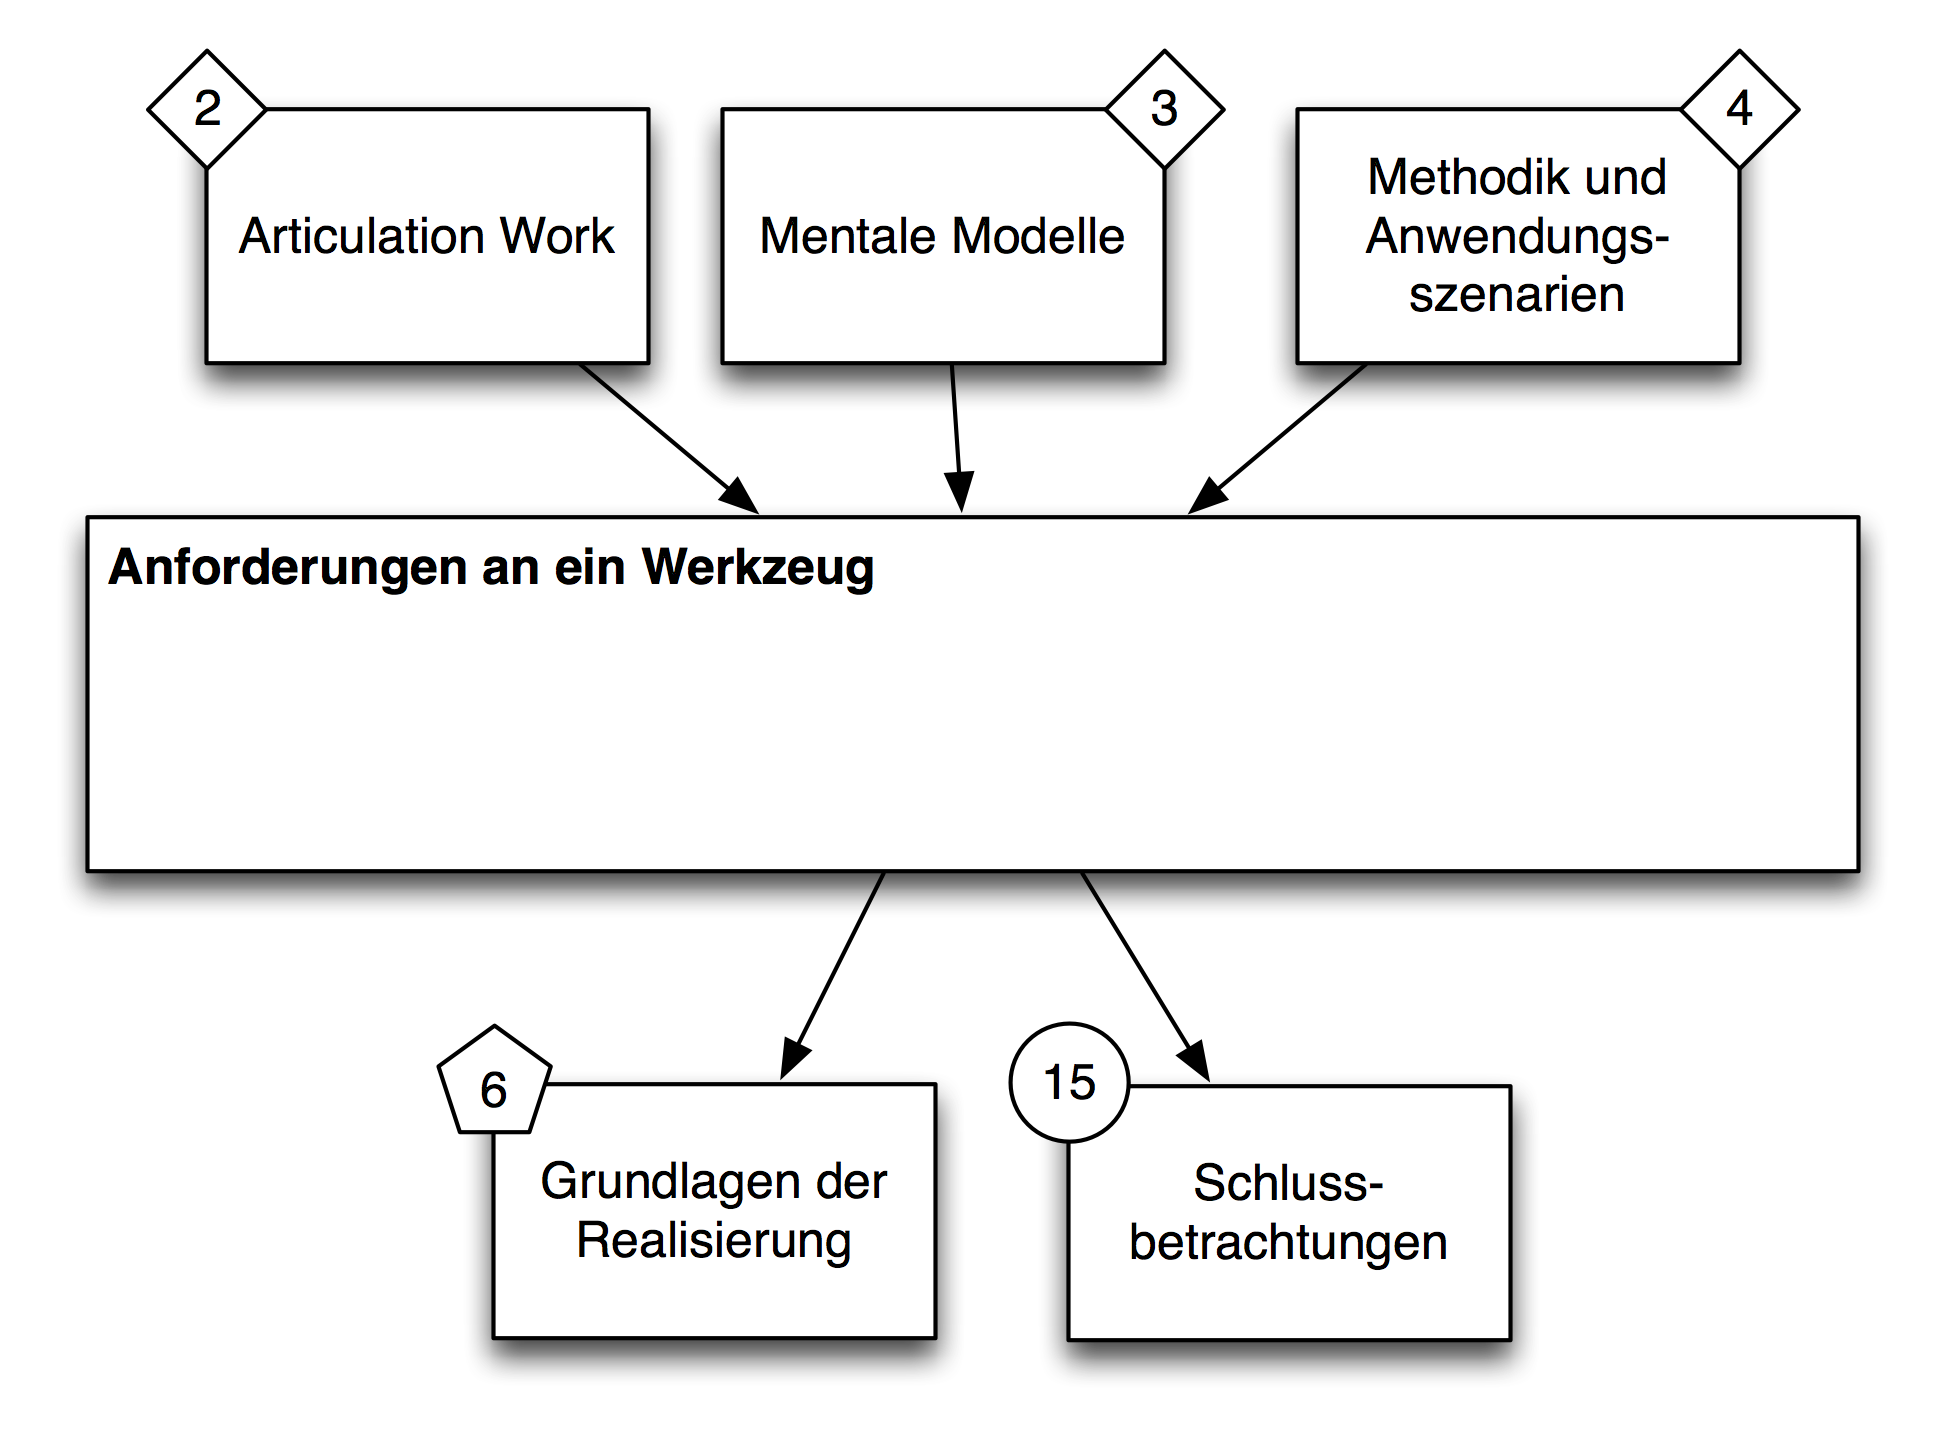
\includegraphics[scale=0.75]{img/Kontextgrafiken/k5.png}
	\caption{Kapitel „Anforderungen an ein Werkzeug“ im Gesamtzusammenhang}
	\label{fig:img_Kontextgrafiken_k5}
\end{figure}

Die Anforderungen lassen sich jeweils auf einen von drei Aspekten zurückführen, die in den Kapiteln \ref{cha:articulation_work} und \ref{cha:mentale_modelle} beschrieben sind. Größtenteils sind sie direkte Konsequenzen auf den Vorgaben hinsichtlich Struktur und Vorgehen, die von Strukturlegetechniken oder Concept Mapping gemacht werden. Es ist jedoch zusätzlich notwendig, auf die zur Durchführung expliziter „Articulation Work“ selbst zurückzugreifen, um die Eignung des Werkzeugs nicht nur für generische Externalisierung von mentalen Modellen selbst sicherzustellen. Vielmehr muss auch die Berücksichtigung der speziellen Anwendungsbedingungen und Betrachtungsgegenstände im Rahmen von „Articulation Work“ gewährleistet werden.

\section{Anforderungen aus Strukturlegetechniken} % (fold)
\label{sec:anforderungen_aus_strukturlegetechniken}

\begin{anf}
	\label{anf:physische_abbildung_legen_beliebiger_diagrammatischer_modelle}
	Physische Abbildung beliebiger diagrammatischer Modelle
\end{anf}
 % (fold)


Ein Werkzeug zur Unterstützung von Strukturlegetechniken muss das grundlegende Konzept der Methodik vollständig unterstützten. Es muss möglich sein, Konzepte auf einer Modellierungs-Oberfläche zu platzieren und zueinander in Beziehung zu setzen. Der gesamte Modellstatus muss visuell auf der Oberfläche erkennbar sein.

% paragraph physische_abbildung_legen_beliebiger_diagrammatischer_modelle (end)

\begin{anf}
	\label{anf:unterstützung_der_iterativen_aushandlung_des_modells}
	Unterstützung der iterativen Aushandlung des Modells
\end{anf}
 % (fold)


Im Sinne der Unterstützung der Dialog-Konsens-Methodik sind ist der Austausch über das Modell durch das Werkzeug zu unterstützen. Vor allem muss es möglich sein, Anmerkungen über Konsens oder Dissens über einzelnen Modellteile oder das gesamte Modell explizit mit in die Repräsentation aufzunehmen. 

% paragraph unterstützung_der_iterativen_aushandlung_des_modells (end)

\begin{anf}
	\label{anf:ermöglichung_experimenteller_veränderungen_am_modell}
	Ermöglichung experimenteller Veränderungen am Modell
\end{anf}
 % (fold)


Es muss möglich sein, das Modell experimentell zu verändern und ggf. zu einem früheren stabilen Modellzustand zurückzukehren. Dies erlaubt eine konsequenzlose Erkundung von Lösungsräumen und unterstützt damit den Dialog-Konsens-Prozess. Das Werkzeug muss also stabile Modellzustände erfassen und deren Rekonstruktion unterstützen.

% paragraph ermöglichung_experimenteller_veränderungen_am_modell (end)

% section anforderungen_aus_strukturlegetechniken (end)

\section{Anforderungen aus Concept Mapping} % (fold)
\label{sec:anforderungen_aus_concept_mapping}

\begin{anf}
	\label{anf:nicht_vorgegebene_semantik_der_modellierungselemente}
	Nicht vorgegebene Semantik der Modellierungselemente
\end{anf}
 % (fold)

Wie oben bereits argumentiert, sind zur Unterstützung von expliziter „Articulation Work“ vor allem Varianten von Strukturlegetechniken geeignet, die im Sinne von Concept Mapping keine Vorgaben hinsichtlich der zu verwendenden Konzepte und Verknüpfungen machen. Das Werkzeug muss dementsprechend die Offenheit bieten, beliebige Klassen von Konzepten und Verknüpfungen zu definieren (z.B. Klasse „organisationale Rolle“) und von diesen beliebige Instanzen zu bilden und zu benennen (z.B. Instanz „Geschäftsführer“). Gleichzeitig muss sichergestellt werden, dass die festgelegte Semantik im Modell mit abgebildet wird und nicht verloren geht.

% paragraph nicht_vorgegebene_semantik_der_modellierungselemente (end)

\begin{anf}
	\label{anf:verknüpfung_mit_digitalen_ressourcen}
	Verknüpfung mit digitalen Ressourcen
\end{anf}
 % (fold)


Die Einbindung von digitalen Ressourcen (Dateien, Hyperlinks,...) ermöglicht die Einbindung des Modells in den organisationalen Kontext und erleichtert so einerseits die Verständnisbildung und ermöglicht andererseits die Verwendung der Repräsentation als unmittelbare Handlungsanleitung mit Verknüpfungen zu den betroffenen Arbeitsgegenständen.

% paragraph verknüpfung_mit_digitalen_ressourcen (end)

\begin{anf}
	\label{anf:bearbeitung_von_beliebig_komplexen_modellen}
	Bearbeitung von beliebig umfangreicher Modellen
\end{anf}
 % (fold)

Umfangreiche Modelle enthalten oft eine große Anzahl von Konzepten und viele Verknüpfungen. Das Werkzeug muss das Modell in einer Form darstellen, die dessen Erfassung und Manipulation ermöglicht, ohne die Repräsentierenden kognitiv zu sehr zu belasten.
% paragraph bearbeitung_von_beliebig_komplexen_modellen (end)

% section anforderungen_aus_concept_mapping (end)

\section{Anforderungen aus Articulation Work} % (fold)
\label{sec:anforderungen_aus_articulation_work}

\begin{anf}
	\label{anf:kollaborative_und_unmittelbare_manipulierbarkeit_des_modells}
	Kooperative und unmittelbare Manipulierbarkeit des Modells
\end{anf}
 % (fold)

Zur Unterstützung von expliziter „Articulation Work“ muss das Werkzeug kooperative Strukturlege-Prozesse erlauben. Es muss möglich sein, das gelegte Modell simultan zu erweitern oder zu verändern.

% paragraph kollaborative_und_unmittelbare_manipulierbarkeit_des_modells (end)

\begin{anf}
	\label{anf:persistente_ablage_des_modells_möglichkeit_zur_rekonstruktion}
	Persistente Ablage des Modells und Möglichkeit zur Rekonstruktion
\end{anf}
 % (fold)

Die persistente Ablage eines Modells (z.B. als digitale Repräsentation) und Werkzeugunterstützung zur Rekonstruktion eines abgelegten Modells erlaubt die Wiederaufnahme eines unterbrochenen Strukturlegeprozesses bzw. die Reflexion und Anpassung bereits erstellter Modelle zu einem späteren Zeitpunkt\footnote{\emph{„By recording and replaying the authoring process, navigable history can re-situate an author after a gap in the authoring process. Similarly, in a collaborative authoring process, an author can play through the events since his/her last authoring session to quickly determine the activity of the other authors. Finally, in many situations, information becomes harder to interpret as its context changes over time. By returning to the state of the information space at the time of authoring, disambiguation of the information may become possible. For the reader who is not also the writer of the hypertext there are additional uses of navigable history. A reader replaying the author’s writing process can gain insight into the motivation of the author and have a greater understanding of the author’s writing style. Such an understanding is important in collaborative work and in other contexts, like education and literary analysis.“} \citep{Shipman00}}.

% paragraph persistente_ablage_des_modells_möglichkeit_zur_rekonstruktion (end)

% section anforderungen_aus_articulation_work (end)

\section{Grundlegende Technologieentscheidung} % (fold)
\label{sec:grundlegende_technologieentscheidung}

Basierend auf den oben identifizierten Anforderungen kann nun eine grundlegende Entscheidung hinsichtlich der Technologie zur Umsetzung der Werkzeugunterstützung getroffen werden. Aufgrund der Anforderungen, die aus dem Bereich der „Strukturlegetechniken“ sowie „Articulation Work“ selbst abgeleitet wurden, ist die Unterstützung durch ein Werkzeug notwendig, das die Erstellung und Repräsentation der Modelle im physischen Raum ermöglicht.

Ein Teil der Anforderungen, die im Bereich des „Concept Mapping“ und ebenfalls wieder der „Articulation Work“ identifiziert werden konnten, können hingegen nur realisiert werden, wenn das Werkzeug mit rechner-unterstützter Funktionalität angereichert wird.

Einerseits ist es nun also notwendig, das Modell physisch abzubilden, was der Verwendung eines Werkzeugs mit  bildschirmbasierter Benutzungsschnittstelle entgegensteht. Andererseits ist zur Umsetzung mancher Anforderungen die Verwendung eines Rechners notwendig, so dass das Modell auch digital erfasst und repräsentiert werden muss.

Ein Ansatz der Mensch-Maschine-Interaktion, der die Verwendung von interaktiven Systemen mit nicht-traditionellen Benutzungsschnittstellen untersucht, ist jener der \emph{„Tangible Interfaces“}. Als „Tangible Interfaces“ werden im Allgemeinen Benutzungsschnittstellen bezeichnet, die ein Computersystem mit auf den jeweiligen Anwendungsfall abgestimmten physischen Artefakten kontrollierbar machen, die gleichzeitig zur Informationsausgabe durch das Computersystem verwendet werden.

Für den hier vorliegenden Anwendungsfall -- der interaktiven kooperativen Erstellung von diagrammatischen Modellen -- bietet sich die Verwendung eines \emph{„Tangible Tabletop Interface“} an. Als Spezialfall eines „Tangible Interface“ wird hier eine Tischoberfläche als Ein- und Ausgabekanal verwendet, auf dem physische Artefakte zur Interaktion mit dem System verwendet werden. Die Ähnlichkeit dieses Ansatzes mit dem Anwendungsszenario im Falle von „Strukturlegetechniken“ lässt eine Verwendung zur Umsetzung der in dieser Arbeit zu entwickelnden Werkzeug als sinnvoll erscheinen. 

% section grundlegende_technologieentscheidung (end)

\section{Zusammenfassung}
\label{sec:anforderungen_zusammenfassung}

In diesem Kapitel wurden die Anforderungen an das zu entwickelnden Werkzeug aus den Ergebnissen der Kapitel \ref{cha:articulation_work}, \ref{cha:mentale_modelle} und \ref{cha:methodik} abgeleitet. Insgesamt konnten \theanf \ Anforderungen identifiziert werden, die hier -- unabhängig von der konkreten Umsetzung -- rein aus Sicht der konzeptionell zu unterstützenden Tätigkeit beschrieben wurden.

Im letzten Abschnitt dieses Kapitels wurde auf Basis der Ergebnisse der Anforderungserhebung jene Klasse von Systemen identifiziert, deren Verwendung die grundlegende Forderung nach physischer Modellbildung und gleichzeitiger Unterstützung durch computerbasierte Werkzeuge erfüllen kann. Der Einsatz von „Tangible Interfaces“ mit ihrem Anspruch, konkrete, physische Benutzungsschnittstellen für interaktive Computersysteme zur Verfügung zu stellen, erscheinen hier am Erfolg versprechendsten zu sein.

In den folgenden Kapiteln wird nun aufbauend auf der Grundsatzentscheidung für die Entwicklung eines „Tangible Interfaces“ das Werkzeug in allen in den Anforderungen angesprochenen Aspekten spezifiziert. Zusätzlich sind auch jeweils die konkrete technische Umsetzung sowie allfällige Einschränkungen, die diese Umsetzung mit sich brachte, beschrieben.

Kapitel \ref{cha:implementierung_Überblick} geht -- noch unabhängig von dem konkreten hier entwickelten Werkzeug -- auf die Eigenschaften von Tangible Interfaces und deren Spezifikation ein. Daneben wird in diesem Kapitel auch die „Related Qork“ aus konzeptioneller und technischer Sicht aufgearbeitet. In den Kapiteln \ref{cha:input_&_interpretation}, \ref{cha:visualisierung} und \ref{cha:persistierung} werden die Implementierungsalternativen und die konkrete Umsetzung des Werkzeugs getrennt für die Eingabe von Information (also die Modellbildung selbst), die Ausgabe von Information sowie die Sicherstellung der Persistierung der Modelle beschrieben. Die Überprüfung der Erfüllung der hier spezifizierten Anforderungen ist Gegenstand der Kapitel \ref{cha:eval_werkzeug} und \ref{cha:eval_modell}, die Teil der Beschreibung der Evaluierung des hier entwickelten Systems sind.

% chapter anforderungen (end)

\chapter{Implementierung – Überblick} % (fold)
\label{cha:implementierung_Überblick}

Wie im Kapitel "Design" gefordert, wurde zur Umsetzung des Werkzeugs ein "Tangible Tabletop Interface" verwendet. Tabletop Interface zeichnen sich im Generellen dadurch aus, dass im Gegensatz zu handelsüblichen Rechnern nicht nur die Software sondern auch die Hardware applikationsspezifisch ist und nicht generisch eingesetzt werden kann. Die Hardware bildet dabei einen Teil oder die gesamte Benutzungsschnittstelle ab. Im speziellen Fall eines "Tangible Tabletop Interfaces" basiert der Benutzerinteraktion auf der Verwendung physischer Bausteine ("Tokens"), die auf der physischen Oberfläche des Interfaces manipuliert werden. Dieses Paradigma wird ergänzt von Tabletop Interfaces, die die Benutzerinteraktion ausschließlich auf Gesten bzw. Berührungen der Oberfläche abbilden (horizontal verbaute "Touch-" bzw. "Multi-Touch-Displays").

\section{Grundlegende \& verwandte Arbeiten} % (fold)
\label{sec:grundlegende_&_verwandte_arbeiten}

REFs!!! Die Entwicklung von Tabletop Interfaces begann Mitte der 1990er-Jahren mit den Arbeiten von Ishii \& Ullmer. Auch die erste Anwendung, die sich mit Modellierungs-Ansätzen mit Hilfe von Tabletop Interfaces konzentriert, stammt aus dieser Zeit. Mit dem fortschreiten der technologischen Entwicklung ist heute ein Status erreicht, in dem mit Hilfe generischer Identifikations-Frameworks schnell und ohne großen Aufwand Applikationen mit "tangiblen" Inputkanälen erstellt werden können. Zur Zeit noch im Prototypenstatus befinden sich Ansätze, die sich mit generischen Möglichkeiten des tangiblen Informationsoutputs beschäftigt. Der Rückkanal vom Rechner zum Benutzer wird heute zumeist mit der Projektion von Inhalten auf die Arbeitsoberfläche umgesetzt.

In den folgenden Abschnitten wird die historische Entwicklung von Tabletop Interfaces sowie der aktuelle Stand der Entwicklung im Anwendungsbereich dieser Arbeit betrachtet. Es werden dabei die grundlegenden Konzepte und Eigenschaften der jeweiligen Arbeiten betrachtet und das Potential hinsichtlich der Umsetzung von in Kapitel XY identifizierten Anforderungen an das hier entwickelte Werkzeug betrachtet. 

\subsection{Tangible Interfaces} % (fold)
\label{sub:tangible_interfaces}

Der Begriff der Tangible bzw. Graspable Interfaces – also der "berührbaren" oder "begreifbaren" Benutzungsschnittstellen — stammt aus der Mitte der neunziger Jahre des zwanzigsten Jahrhunderts. \citet{Fitzmaurice95} werden im Allgemeinen als die ersten betrachtet, die den Begriff des "Graspable User Interfaces" prägen und damit die Manipulierbarkeit digitaler Information durch physische Mittel beschreiben. \citet{Fitzmaurice96} präzisiert später den Begriff durch die Abgrenzung zwischen (herkömmlichen, maus-, tastatur- und bildschirmbasierenden) zeitlich gemultiplexten Schnittstellen, bei denen der Informationsaustausch zwischen Benutzer und System über einen Kanal zeitlich hintereinander erfolgt und den (neuartigen, berührbaren) räumlich gemultiplexten Schnittstellen, bei denen mehrere Kanäle gleichzeitig zur Interaktion zwischen Benutzer und System verwendet werden können. 

Der Begriff des "Tangible User Interfaces" wurde kurz danach bzw. parallel dazu von \citet{Ishii97} eingeführt. \citeauthor{Ishii97} verfolgen dabei bei der Definition den umgekehrten Weg und sprechen von einer "Augmentation der realen Welt durch eine Kopplung von digitaler Information and physische Objekte"\footnote{\emph{“augment the real physical world by coupling digital information to everyday physical objects and environments”}\citep{Ishii97}}. 

% subsection tangible_interfaces (end)

\subsection{Historische Entwicklung von Tabletop Interfaces} % (fold)
\label{sub:historische_entwicklung_von_tabletop_interfaces}

\paragraph{Sensetable} % (fold)
\label{par:sensetable}
Der Sensetable \citep{Patten01}
% paragraph sensetable (end)

\paragraph{BUILD-IT} % (fold)
\label{par:build_it}
\citep{Fjeld01}
% paragraph build_it (end)
% subsection historische_entwicklung_von_tabletop_interfaces (end)

\subsection{Tangible Interfaces zur Modellbildung} % (fold)
\label{sub:tangible_interfaces_zur_modellbildung}

% subsection tangible_interfaces_zur_modellbildung (end)

\subsection{Aktuelle verwandte Ansätze} % (fold)
\label{sub:aktuelle_verwandte_ansätze}

% subsection aktuelle_verwandte_ansätze (end)
\begin{itemize}
	\item Historische Entwicklung von Tabletop Interfaces
	\begin{itemize}
		\item Sensetable
		\item Morten Fjeld
		\item ReacTable
		\item Eva Hornecker
	\end{itemize}
	\item Historische Entwicklung von Tangible Interfaces zur Modellbildung
	\begin{itemize}
		\item Sensetable Modeling Application
		\item Designer's Outpost (Klemmer)
	\end{itemize}
	\item Aktuelle verwandte Ansätze
	\begin{itemize}
		\item Antle (TEI Mail-Pointer)
		\item Sun (TEI Demo)
	\end{itemize}
\end{itemize}


% section grundlegende_&_verwandte_arbeiten (end)

% chapter implementierung_Überblick (end)
\chapter{Input \& Interpretation} % (fold)
\label{cha:input_&_interpretation}
In diesem Kapitel wird jener Teil des Werkzeuges beschrieben, in dem die Interaktion der der Benutzer mit dem Werkzeug erfasst und interpretiert wird. Der erste Abschnitt behandelt grundlegende Möglichkeiten zur Erfassung der Benutzerinteraktion auf tisch-basierten Benutzungsschnittstellen und endet mit der Identifikation der im konkreten Anwendungsfalls geeignetsten Technologie. Diese wird durch die Beschreibung von dafür verfügbaren Frameworks konkretisiert, was letzendlich in der Entscheidung für ein konkretes Produkt mündet.

Basierend auf dieser Entscheidung wird in den folgenden beiden Abschnitten auf das Design der Hard- und Softwarekomponenten eingegangen, die unmittelbar der Eingabe von Information durch Benutzer dienen. Der Ausgabeaspekt wird hier bewusst ausgeklammert und im nächsten Kapitel beschrieben. Dieses Kapitel endet mit eine Beschreibung der Interpretationsroutinen, die aus den durch das Framework gelieferten Rohdaten höherwertige, anwendungsspezifische Information extrahieren und diese den nachgeordneten Software-Modulen zur Verfügung stellen.

\section{Möglichkeiten zur Erfassung von Benutzerinteraktion} % (fold)
\label{sec:möglichkeiten_zur_erfassung_von_benutzerinteraktion}

Im Gegensatz zu Systemen mit dezidierten Eingabegeräten (wie Tastatur oder Maus) ist die Informationseingabe bei Tangible Interfaces unmittelbar an physische Tokens gebunden, die unabhängig voneinander und gegebenenfalls auch simultan manipuliert werden können. Diese Manipulation wird von einer vorhandenen Infrastruktur erfasst und im Sinne von Eingabedaten interpretiert. Der wesentliche Unterschied zu dezidierten Eingabegeräten besteht darin, dass die Manipulation des physischen Artefakts selbst für den Benutzer bedeutungstragend ist und nicht nur dem Zweck einer Zustandsänderung des digitalen Informationsraums dient. Dies impliziert, dass der Zustand der verwendeten Tokens bzw. der aktuelle Wert deren relevanten Parameter (z.B. Position, Rotation, Form, ...) erfasst werden kann, ohne die Bedeutung der Tokens noch deren Manipulierbarkeit in der realen Welt zu beeinflussen. Je nach Anwendungsfall kommen dafür mehrere Unterschiedliche technologische Ansätze in Frage. Die Beurteilungskriterien die dabei zu berücksichtigen sind, liegen nicht nur in den zu erhebenden Parametern begründet sondern umfassen auch die notwendige Erfassungsrate des Zustandes der Tokens sowie die Anzahl der simultan zu erfassenden Tokens bzw. Eigenschaften.

Im konkreten System muss - wie in Kapitel XY beschrieben - die planare Position von mehreren Tokens in Echtzeit (d.h. mehrmals pro Sekunde mit für den Benutzer nicht wahrnehmbaren Verzögerungen) erfasst werden. Neben der Position ist noch die Rotation eines Tokens als Raumparameter von Interesse. Bezüglich des Zustands eines Tokens muss erfasst werden können, ob es geöffnet oder geschlossen ist und ob es eingebettete Objekte enthält oder nicht. Mit diesen Anforderungen wird in den folgenden Unterabschnitten ein technologischer Ansatz zur Umsetzung der Interaktionserkennung ausgewählt.

\subsection{In Frage kommende technologische Ansätze} % (fold)
\label{sub:potentielle_technologische_ansätze}
Bei der Auswahl möglicher technologischer Ansätze zur Erfassung der Benutzerinteraktion müssen die zu erfassenden Parameter unterschiedlich behandelt werden. Konkret werden hier Ansätze zur Erfassung der Raumparameter (Position, Rotation) und Ansätze die Zustandsänderungen des Tokens erfassbar machen unterschieden. 

\subsubsection{Raumparameter} % (fold)
\label{ssub:raumparameter}
\index{Positionsbestimmung} 
Zur Erfassung von Raumparametern von Tokens bieten sich mehrere technologische Ansätze an. In Frage kommen für das konkrete - tisch-basierte System - nur Technologien, die eine Erfassung dieser Parameter mit einer Genauigkeit im Zentimeter- bis Millimeter-Bereich ermöglichen, da eine niedrigere Raumauflösung zu zu großen Ungenauigkeiten in der Positionsbestimmung führen würden, die einen Einsatz für das hier vorgestellte Werkzeug nicht erlauben würden. Im Folgenden werden die in Frage kommenden Technologien in ihren Grundzügen beschrieben und hinsichtlich ihrer Eignung für das konkrete System bewertet.

\paragraph{Optisch} % (fold)
\label{par:optisch}
\index{Positionsbestimmung!optisch} 
\index{Barcode} 

Optische Positionsbestimmung erfolgt immer mit Hilfe von Kamera-Systemen und Methoden der digitalen Bildverarbeitung. Die Kamera erfasst dabei die zu identifizierenden Tokens, dass resultierende Bild wird mit in Software umgesetzten Algorithmen ausgewertet, wodurch zumindest Identität und Position, zumeist aber auch weitere Raumparameter (wie Rotation) aller im Kamerabild befindlichen Tokens ermittelt werden können. Die Erkennung ist dabei auf den Erfassungsbereich der Kamera beschränkt. Neben diesem Einflussfaktor bestimmen zudem die Auflösung der Kamera sowie die Größe der Tokens die letztendlich erfassbare Fläche. Optische Systeme sind generell bei schlechten oder wechselnden Lichtverhältnissen eher fehleranfällig und nicht robust gegen Verdeckungen von Tokens (etwa durch Gliedmaßen oder andere Tokens).

Hinsichtlich des Identifikationsansatzes können zwei Arten von Systemen unterschieden werden. \emph{Codebasierte} Systeme verwenden zur Identifikation eines Tokens einen von der Kamera erfassbaren Code (etwa einen "Barcode"), der eindeutig einem Token zugeordnet werden kann. \emph{Featurebasierte} Systeme identifizieren ein Token aufgrund seiner äußeren Eigenschaften, zumeist über dessen Form (Schattenriss). Letztere bieten den Vorteil, dass ein Token nicht durch das Anbringen eines zusätzlichen Codes optisch verändert werden muss. Der größte Nachteil besteht in der Eigenschaft, dass nur Token mit unterschiedlichen Formen eindeutig identifiziert werden können. Die eindeutige Identifikation von mehreren Tokens einer Bauart ist bei featurebasierten Systemen nicht möglich. Codebasierte Systeme verwenden zumeist nicht herkömmliche Barcodes sondern robustere Systeme, bei denen eine Erkennung auch unter widrigen Beleuchtungsbedingungen oder niedrigen Bildauflösungen möglich ist und die zum Teil auch die Extraktion zusätzliche Information über weitere Raumparameter (wie Rotation, teilweise auch Parameter der dritten Dimension wie Neigung oder Entfernung) ermöglichen. 

Codebasierte Systeme können hinsichtlich der Art der Codierung der Indentitätsinformation wiederum in zwei Klassen unterschieden werden. Eine Gruppe von Ansätzen integriert die eigentliche Nutzinformation, also im Wesentlichen die tokenspezifische Identifikationsnummer, direkt in den Code und ermöglicht so ein direktes Auslesen der Information (z.B. bei QRCode (REF)). Die zweite Gruppe verwendet eine indirekte Zuordnung zwischen Token-ID und Code. Bei derartigen Ansätzen muss die Identität eines Tokens in einem Zwischenschritt über eine Mapping-Tabelle abgebildet werden, im Gegenzug ist die Ausgestaltung des Codes flexibler, im Allgemeinen kann dabei eine höhere Robustheit bei der Erkennung erreicht werden (z.B. ARToolkit (REF)).

% paragraph optisch (end)

\paragraph{Kapazitiv} % (fold)
\label{par:kapazitiv}
\index{Positionsbestimmung!kapazitiv}  

Kapazitive Ansätze basieren auf der Änderung der Kapazität von Leiterbahnen, die durch deren Berührung mit leitfähigem Material verursacht wird. Ursprünglich wurde die Technologie zur Umsetzung von berührungssensitiven Oberflächen entwickelt, kann jedoch auch zum Tracking von Tokens verwendet werden. Im Gegensatz zu druckempfindlichen Oberflächen (klassischen "Touchscreens") ist keine Druckausübung zur Erkennung notwendig, es können außerdem auch mehrere Tokens (bzw. Finger) gleichzeitig erkannt werden.

Technologisch bedingt müssen bei kapazitiven Ansätzen alle zu identifizierenden Objekte die Oberfläche des Systems berühren. In dieser Oberfläche ist ein Metallgitter eingebettet, zwischen dessen Adern eine elektrische Kapazität gemessen werden kann. Diese Kapazität verändert sich, sobald diese Adern berührt werden (wobei die Token in einen entsprechend geeigneten Material ausgeführt sein müssen). Durch die lokale Änderung der Kapazität kann die Position einer Berührung festgestellt werden. Die Genauigkeit ist dabei durch die Rasterweite des Metallgitters eingeschränkt. Der größte Nachteil eines kapazitiven Ansatzes ist in diesem Kontext aber, dass die Identität eine Tokens nicht direkt festgestellt werden kann (die Kapazitätsänderung ist für alle Token identisch). Zudem ist die Extraktion weiterer Raumparameter (wie Rotation) nicht bzw. nur mit zusätzlichen Aufwand möglich. Die Vorteile von kapazitiven Systemen liegen in der hohen Robustheit der Erkennung auch bei widrigen Umgebungseinflüssen (Lichtverhältnisse, Schmutz) sowie der prinzipiell beliebig großen und beliebig geformten Oberfläche, die zur Erkennung verwendet werden kann.

Kapazitive Systeme eignen sich also zur Positionsbestimmung, nicht aber zur Identifikation von Tokens. Dies macht sie für den konkreten Anwendungsfall nur in Kombination mit einer anderen Technologie geeignet. 

% paragraph kapazitiv (end)

\paragraph{Elektromagnetisch} % (fold)
\label{par:elektromagnetisch}
\index{Positionsbestimmung!elektromagnetisch} 
\index{RFID}
 
Die Ausstattung von Tokens mit elektromagnetisch erfassbaren Einheiten (z.B. RFID-Chips) ermöglicht ebenfalls die Erfassung von Raumparametern. Vorrangig eignet sich diese Technologie jedoch zur Identifikation von Tokens, die Positionsbestimmung kann nur mit erheblichem technischen Aufwand durchgeführt werden.

RFID-Chips (als Beispiel für einen elektromagnetischen Ansatz) sind passive Bauteile, die bei Energieversorgung durch ein elektrisches Feld aktiv werden und ihrerseits eine eindeutige Identifikationsnummer senden (im einfachsten Fall, komplexere Varianten sind möglich, werden hier aber nicht betrachtet). Historisch stammt die Technologie aus der Logistik und Warenwirtschaft und dient der Identifikation von Gütern und nicht der exakten Positionsbestimmung. Diese ist somit auch nur mittels erweiterter Infrastruktur möglich. Zum Auslesen eines RFID-Chips wird ein Lesegerät mit Antenne benötigt. Aus der Feldstärke, mit der diese Antenne die Antwort des Chips empfängt, kann auf die Entfernung des Chips von der Antenne geschlossen werden. Durch Kreuzpeilung mit mindestens zwei Antennen, deren Position bekannt ist, kann somit auf die ungefähre Position des Chips (und damit des Tokens, in das dieser eingebaut ist) geschlossen werden. Durch den Einsatz von "Antennenarrays" (matrixförmig angeordneten Antennen) mit geringer Reichweite ist so eine verhältnismäßig exakte (Größenordnung einige cm) Positionsbestimmung möglich. Die Feststellung der Ausrichtung eines Tokens (Rotation) ist auf diesem Wege allerdings nicht möglich. Die Identifikation eines Tokens ist jedoch unabhängig von Sichtkontakt und unmittelbarer Berührung und somit äußerst robust gegen Umgebungseinflüsse.

Elektromagnetische Systeme eignen sich wegen des hohen technischen Aufwandes bei gleichzeitig beschränkter Genauigkeit nur bedingt zur Feststellung von Raumparametern. Durch die Ausrichtung auf Extraktion der Identitätsinformation ist der Ansatz jedoch gut zur Kombination mit anderen Technologien wie kapazitiven Ansätzen geeignet, die ihre Stärken in der Bestimmung der Raumparameter haben.
 
% paragraph elektromagnetisch (end)

\paragraph{Akustisch} % (fold)
\label{par:akustisch}
\index{Positionsbestimmung!akustisch} 
\index{Ultraschall} 

Akustische Ansätze zur Positionsbestimmung basieren im Generellen auf der Laufzeitmessung von Ultraschallwellen im Raum. Mit entsprechender Infrastruktur ist damit in einem begrenzten Bereich ein hochexakte Feststellung der Raumparameter in drei Dimensionen (Genauigkeit im mm-Berich) sowie die Identifikation von Tokens möglich.

Ultraschallbasierte Techniken zur Positionsbestimmung basieren auf dem Einsatz von Bakensendern an bekannten Positionen. Diese Sender werden zumeist an der Zimmerdecke montiert und senden periodisch einen Ultraschallimpuls aus. Dieser Impuls wird von den Tokens (die in diesem Fall aktive Bauteile mit Stromversorgung sind) empfangen, die daraufhin einen sie identifizierenden Impuls zurücksenden. Aus der Laufzeit zwischen Absetzen des Sendeimpuls und Empfangen des Antwortimpulses bei verschiedenen Baken lässt sich so die Position des Tokens im Raum feststellen. Problematisch ist hierbei jedoch die durch den auf sequentieller Zeitmessung basierenden Ansatz beschränkte Anzahl von verfolgbaren Tokens, wenn Echtzeit-Ansprüche gestellt werden. Zudem ist der Ansatz nicht robust gegen (akustisch) verdeckte Tokens. Eine Anfälligkeit gegenüber anderen Störeinflüssen besteht nicht. 

Für die Feststellung von Raumparametern sind ultraschall-basierte Systeme generell ausgezeichnet geeignet. Auch die Identifikation von Tokens ist prinzipiell möglich. Bei der Bewertung hinsichtlich des Einsatzes für tisch-basierte Systeme ist jedoch zu bedenken, dass eine drei-dimensionale Positionierung nicht zu den allgemeinen Anforderungen zählt und nur in speziellen Anwendungsfällen sinnvoll sein kann. Zudem kann die Notwendigkeit von stromversorgten Tokens einen Nachteil bzw. ein Hindernis beim Einsatz darstellen.

% paragraph akustisch (end)

\paragraph{Bewertung} % (fold)
\label{par:bewertung}

Im konkreten Anwendungsfall ist die Feststellung der Identität sowie der planaren Position und Rotation von mehreren Tokens in hoher Genauigkeit sowie in Echtzeit gefordert. Aus oben genannten Gründen sind kapazitive und elektromagnetische Systeme im Einzeleinsatz nur bedingt geeignet. Akustische Systeme erscheinen für den Anwendungsfall als zu aufwändig und unflexibel und stoßen außerdem bei der Anzahl der simultan zu verfolgenden Tokens an ihre Grenzen.

Die Kombination von kapazitiven und elektromagnetischen Systemen ist grundsätzlich eine Möglichkeit, die in Betracht gezogen werden könnte. Auch optische Systeme genügen den Anforderungen und kommen damit in Frage. Der kombinierte Ansatz ist im Vergleich mit optischen Systemen als robuster gegen Störeinflüsse aus der Umgebung zu betrachten. Für optische Systeme sprechen hingegen die weitaus geringeren Aufwände für Infrastruktur und Tokens sowohl bei Anschaffung als auch bei Wartung und Betrieb. Durch die geringere Komplexität des Systems sind auch weniger potentielle Fehlerquellen vorhanden, was bei der Erstellung des Werkzeug-Prototypen hilfreich ist. Aufgrund dieser Aspekte und einer vergleichbaren zur erwartenden Erkennungsleistung wurde für die hier vorgestellten Anwendungfalls die Entscheidung getroffen, ein optisches System zur Bestimmung der Positionsparameter sowie der Identität der Tokens einzusetzen.

% paragraph bewertung (end)

% subsubsection raumparameter (end)

\subsubsection{Tokenzustand} % (fold)
\label{ssub:tokenzustand}

Hinsichtlich des Tokenzustands sind im Kontext des hier vorgestellten Anwendungsfall Informationen zu erheben, die den Inhalt des Tokens betreffen. Wie in Kapitel XY beschrieben sind die Modellierungs-Tokens als Container ausgeführt, die geöffnet und geschlossen werden können und in die kleiner Tokens als Trägen von Zusatzinformation hineingelegt werden können. Die Auswahl eines Ansatzes, der die Identifikation des Öffnungs-Zustandes eines Tokens sowie dessen Inhalt erlaubt, ist Gegenstand dieses Abschnitts. Dazu wird grundlegend zwischen dem Einsatz von passiven Tokens und aktiven Tokens unterschieden. Passive Tokens besitzen keine zusätzliche Elektronik, die geforderten Informationen können lediglich durch die bereits vorhandene (optische) Infrastruktur festgestellt werden. Aktive Tokens werden hingegen mit zusätzlicher Elektronik zur Zustandsbestimmung ausgestattet, was allerdings eine Energieversorgung jedes Tokens bedingt.

\paragraph{Passive Token} % (fold)
\label{par:passive_token}
\index{Token!passive}
 
Bei passiven Tokens muss sichergestellt werden, dass die bereits vorhandene Infrastruktur die Zustandsänderungen eines Tokens erfassen kann. Das die vorhandene Infrastruktur auf optischen Technologien basiert, müssen sich alle Zustandsänderungen im äußeren - durch die Kamera erfassbaren - Erscheinungsbild eines Tokens wieder spiegeln.

Der Öffnungszustand eines Tokens kann durch Kameras einfach erfasst werden, wenn sich - je nach eigesetzter Technologie - durch das Öffnen der Umriss des Tokens verändert oder ein weiterer Code sichtbar wird bzw. der bestehende Code modifiziert wird. Diese Anforderung kann also durch passive Tokens erfüllt werden.

Zur Erfassung des Inhalts eines Container-Tokens sind zwei Ansätze denkbar. Einerseits kann der Inhalt eines Tokens zu einem bestimmten Zeitpunkt erfasst werden, andererseits ist auch eine Erfassung der Änderung des Tokeninhalts möglich (Erfassung des Vorgangs von Hineinlegen und Herausnehmen). Diese beiden Möglichkeiten sind hinsichtlich der Umsetzbarkeit mit passiven Token unterschiedlich zu beurteilen. Eine Erfassung das aktuellen Tokeninhalts ist mit optischen Systemen nur schwer möglich. Die einzige sich bietende Möglichkeit ist die von transparenten Teilbereichen der Außenfläche eines Tokens. Damit ist es grundsätzlich möglich, den Inhalt eines Tokens mit einer externen Kamera zu erfassen, sowohl bei feature- als auch code-basierten Ansätzen sind jedoch Verdeckungen, Verzerrungen oder zu geringe Kameraauflösung potentiell problematisch und lassen diesen Ansatz für den praktischen Einsatz als ungeeignet erscheinen.

Die Erfassung der Änderung des Tokeninhalts lässt sich mit optischen Systemen einfach implementieren. So kann der Vorgang des Hineinlegens als auch des Herausnehmens von einer Kamera erfasst werden. Die größte Herausforderung hierbei ist die Identifikation des Tokens, das eingebettet wird. Hier kann es wiederum durch Verdeckungen zu Erkennungsschwierigkeiten führen, was in diesem Fall einen permanent fehlerhaften Modellzustand zur Folge hat, der sich im Falle wiederholter Fehlerkennungen sogar inkrementell verschlimmern kann. Diesem Umstand kann lediglich durch eine explizite Aktion des Benutzers Rechnung getragen werden, der das betreffende einzubettende Token ins Sichtfeld der Kamera halten muss, bis das System Feedback über eine erfolgreiche Erkennung gibt. Diese Lösung erscheint allerdings hinsichtlich der Anforderung, die Technologie für den Benutzer vollkommen in den Hintergrund treten zu lassen, als eher suboptimal.

% paragraph passive_token (end)

\paragraph{Aktive Token} % (fold)
\label{par:aktive_token}
\index{Token!aktive}

Aktive Tokens beinhalten zusätzliche Sensorik, die die Erfassung des Tokenzustands ermöglicht. Derartige Tokens benötigen allerdings eine Energieversorgung und müssen über eine Möglichkeit zur Datenübertragung verfügen, um den Tokenzustand an das System zu übermitteln. Weiters ist im Allgemeinen eine Steuereinheit notwendig, um die Sensoren zu kontrollieren, die Daten zu aggregieren und letzendlich zu übertagen.

Im konkreten Fall einer optisch arbeitenden Infrastruktur bietet sich eine (ggf. aufladbare) Batterie als Energiequelle an, um im Kamerabild Verdeckungen durch ansonsten eventuell zu verwendende Kabel zu vermeiden. Eine Stromversorung über die Oberfläche (wie z.B. im Smart PINS (Gellersen REF) Ansatz vergestellt) scheidet hier aus, da die Blöcke dann mit Krafteinsatz auf die Oberfläche gesetzt werden müssten und nicht verschoben werden können. 

\index{SmartIT} 
Als Steuerungseinheit bietet sich neben selbst auf der Basis von Mikrocontrollern wie dem PIC oder 8051 (REFs) konzipierten Systemen auch Plattformen an, die explizit für den Anwendungszweck der Ansteuerung von Sensoren oder Aktuatoren und der Kommunikation mit einem Basissystem gefertigt werden. Exemplarisch kann hier die Smart-ITs-Plattform (REF) angeführt werden, die neben der flexiblen Ansteuerbarkeiten von unterschiedlichen Sensoren bereits Module zur Vernetzung untereinander und mit zentralen Diensten in der Infrastruktur anbietet.

\index{ZigBee} 
\index{Bluetooth} 
Aus den eben angeführten Gründen erscheint zur Datenübertragung eine drahtlos arbeitende Technologie am geeignetsten. Aufgrund der geringen benötigten Reichweite und der Anforderung, möglichst energieeffizient zu arbeiten, bieten sich die Technologien "Bluetooth" und "ZigBee" an. Bluetooth erreicht höhere Übertragungsraten, ist aber in der Anzahl der gleichzeitig verwendbaren Geräte (max. 7) für den hier vorgestellten Anwendungsfall zu beschränkt. Ein ZigBee-Netz kann mit bis zu 255 Geräten gleichzeitig arbeiten und ist außerdem im Einsatz energiesparender. Für den gegebenen Anwendungsfall erschiene also ZigBee als geeignete Technologie (und wurde auch bereits in (AON Cube, Simon Vogl REF) in einem ähnlichen Anwendungsfall erfolgreich eingesetzt).

Zur Feststellung des Öffnungsstatus eines Container-Tokens bieten sich bei aktiven Sensortechnologien mehrere Möglichkeiten an. Der Einsatz eines Schaltelements, das beim Öffnen den Kontakt herstellt oder unterbricht, erscheint als eine nahe liegende Lösung. Auch der Einsatz eines Drehelements am Angelpunkt des Öffnungsschaniers, dessen elektrische Eigenschaften (z.B. Widerstand oder Kapazität) mit dem Öffnungswinkel ändern, kann angedacht werden. Damit ist nicht nur eine Unterscheidung zwischen "offen" oder "geschlossen" sondern auch die Identifikation von Zwischenzuständen möglich.

Der Inhalt eines Container-Tokens kann ebenfalls mit unterschiedlichen Technologien erfasst werden. Die Zielsetzung ist hier nicht der Positionsbestimmung der eingebetteten Tokens sondern lediglich die Feststellung derer Identität. Naheliegend ist hierzu der Einsatz von elektromagnetischen Ansätzen wie oben beschrieben. Durch das Anbringen von z.B. RFID-Chips an den einzubettenden Tokens sowie eines Lesegeräts im Container-Token kann die Identifikation robust durchgeführt werden. Alternativ bieten sich Systeme an, die auf Gewichtsmessung basieren. Über einen in das Containertoken eingebauten Sensor wird dabei das Gesamtgewicht der eingebetteten Tokens bestimmt. Bei entsprechender Konzeption der einzubettenden Tokens (unterschiedliche Gewichte) kann aus dem Gesamtgewicht auf die tatsächlich enthaltenen Tokens geschlossen werden. Ein Nachteil dieses Ansatzes ist die beschränkte Anzahl von Tokens und die notwendige exakte Fertigung jedes einzelnen Tokens, da es bei Gewichtsabweichungen zu Fehlerkennungen kommt.

% paragraph aktive_token (end)

\paragraph{Bewertung} % (fold)
\label{par:zustand_bewertung}

Hinsichtlich der erreichbaren Flexibilität und zu erwartenden Servicequalität wäre in diesem Abschnitt eine Entscheidung zugunsten aktiver Tokens zu treffen. Im Gesamtkontext betrachtet und unter Berücksichtigung der Entscheidung für optische Systeme zur Bestimmung der Positionsparameter ist diese Wahl jedoch zu relativieren. Wie oben beschrieben, erlaubt eine auf optischen Systemen beruhende Infrastruktur grundlegend die Umsetzung der geforderten Funktionalität. Gleichzeitig wird die Komplexität des Systems massiv reduziert und die Erstellung zusätzlicher Tokens vereinfacht (da keine zusätzliche Elektronik notwendig ist). Der Wegfall von Energieversorgung und Sensorlogik in den Token reduziert deren Gewicht und ermöglicht gleichzeitig mehr Platz für einzubettende Tokens.

Für den hier beschriebenen Anwendungsfalls bzw. die prototypische Umsetzung des Werkzeugs wird deshalb auf aktive Tokens verzichtet und der Einsatz von passiven Tokens bevorzugt. Der Mehraufwand in Erstellung und Wartung des Systems beim Einsatz aktiver Tokens wiegt in der Gesamtheit betrachtet die zu erwartende höhere Erkennungsqualität nicht auf.
% paragraph zustand_bewertung (end)
% subsubsection tokenzustand (end)

% subsection potentielle_technologische_ansätze (end)
\subsection{In Frage kommende Frameworks} % (fold)
\label{sub:verfügbare_frameworks}

Unter Anbetracht der im vorherigen Abschnitt getroffenen grundlegender Technologieentscheidung zugunsten optischer Erkennungstechnologie mit passiven Tokens werden nun unterschiedliche Frameworks betrachtet, die die Umsetzung dieses Ansatzes erlauben. Es sind dabei zwei Klassen von Frameworks zu unterscheiden. \emph{Generische Frameworks für Tangible Interfaces} beschäftigen sich generell mit dem zur Verfügung stellen von Services, die Kopplung von Sensoren und Aktuatoren mit Interpretations-Logik und letzendlich konkreten Applikationen erlauben. Sie gehen dabei nicht auf konkrete  Sensortechnologie (wie die hier verwendeten optischen Ansätze) ein sondern versuchen eine Abstraktionsebene einzuführen, die die Applikationen von der konkreten Technologie entkoppelt und damit flexibler macht. \emph{Frameworks für video-basierten Input für Tangible Interfaces} sind hochspezialisierte Produkte, die konkret für die Umsetzung von optischen Ansätzen zur Eingabe von Daten bei Tangible Interfaces entwickelt werden. Ihr Vorteil liegt im durch die Spezialisierung im Allgemeinen geringeren Aufwand zur Einrichtung und auch während des Betriebs. Echtzeit-Anforderungen sind oft nur mit spezialisierten Frameworks zu erreichen. Eine Kombinationsmöglichkeit zwischen Produkten der beiden Kategorien ergibt sich beim Einsatz eines spezialisierten Frameworks als Eingabe-Modul für eine generisches Framework. Durch diesen Ansatz kann die einfache Inbetriebnahme spezialisierter Frameworks mit der Flexibiltiät generischer Frameworks zusammengeführt werden. 

\subsubsection{Generische Frameworks} % (fold)
\label{ssub:generische_frameworks}

Generische Frameworks zur Behandlung von Input und Output bei Tangible Interfaces sind historisch nicht exakt von anderen Frameworks abzugrenzen, die im Umfeld des Ubiquitous bzw. Pervasive Computing entwickelt wurden. Derartige Ansätze wurden erstmals im Zusammenhang mit "Context Computing" erwähnt, um Applikationen eine generische Möglichkeit zu bieten, Information aus der Umgebung über beliebige Sensoren zu erfassen und diese zu aggregieren und zu interpretieren. Aufbauend auf dieser Interpretation sollen Aussagen über den aktuellen Zustand der Umgebung (den "Kontext") getroffen werden können, die diese Applikationen zur Adaption benutzen können. Der Rückkanal, also die Ansteuerung von Aktuatoren, wurde erst in späteren Entwicklungen berücksichtigt. Die meisten Systeme dienen explizit nicht der Erstellung von marktreifen Applikationen sonderen widmen sich eher der Umsetzung von "Rapid Prototyping"-Ansätzen im Bereich der Tangible Interfaces. Begründet wird dies mit der oft suboptimalen Ressourcen-Ausnutzung, die mit der Generalisierung und Flexiblisierung des Frameworks einhergeht. 

Die Aufzählung der hier beschriebenen Frameworks erhebt keinen Anspruch auf Vollständigkeit. Es wurde eher darauf geachtet, historische bzw. für den konkreten Anwendungsfall geeignete Ansätze aufzunehmen und in ihren wesentlichen Eigenschaften zu beschreiben.

\paragraph{Context Toolkit} % (fold)
\label{par:context_toolkit}
\index{Context Toolkit}
 
Das Context Toolkit \citep{Dey01} ist das historisch erste Framework, das versucht, die starre Verbindung zwischen Sensoren und Applikationslogik aufzubrechen und eine konfigurierbare Schicht einzuziehen, die eine schnellere, generischere Applikationsentwicklung ermöglicht und die Wiederverwendbarkeit einmal entwickelter Komponenten erhöht.

Konzeptuell existieren im Framework drei Arten von Komponenten: Context Widgets, Context Interpreters und Context Aggregators. Context Widgets implementieren die Ansteuerung beliebiger Software- und Hardwaresensoren und sind für das Sammeln von Information über die Umgebung zuständig. Sie vermitteln zwischen der physischen Umgebung und den konzeptuell höher liegenden Komponenten indem sie die unverarbeiteten Kontextdaten mittels einer geeigneten Schnittstelle kapseln und bestimmte Funktionen zur ersten Auswertung der Rohdaten ausführen. Eine Anwendung kann diese Daten verwenden, ohne dass sie Detailkenntnisse über die zugrunde liegenden Sensortechnologien haben muss. Context Interpreter aggregieren die Sensordaten zu komplexeren Kontextinformationen d.h. sie konvertieren und interpretieren die Daten mehrerer Context Widgets und versuchen diese zu einheitlichen Clustern zusammenzufassen. Context Aggregators dient der Zusammenführung verschiedener Kontextinformationen die für bestimmte Anwendungen relevant sind. Context Aggregators bilden damit die Schnittstelle zu den eigentlichen Applikationen.

Das Context Toolkit bietet nicht nur eine Softwareschnittstelle zu physischen Sensoren, es trennt auch die Akquisition und Repräsentation von der Auslieferung der Daten an kontextsensitive Applikationen.
% paragraph context_toolkit (end)

\paragraph{SiLiCon Context Framework} % (fold)
\label{par:silicon_context_framework}

Das SiLiCon Context Framework \citep{Beer03} ist ein Vertreter jener Klasse von Frameworks, deren Verhalten zur Laufzeit dynamisch konfigurierbar sind. Dies bedeutet im konkreten Fall, dass Applikationen die auf Basis des SiLiCon Context Framework erstellt wurden ihr Verhalten und ihren Aufbau aufgrund eintretender Ereignisse verändern können. Dies betrifft sowohl das Aktivieren und Deaktivieren von Input- und Output-Kanälen also auch die Interpretation der eingehenden Information und die Reaktion darauf. Das Framework wurde entworfen, um Szenarien zu beschreiben, in denen interaktive Systeme kontextsensitiv - d.h. abhängig vom aktuellen Zustand ihrer Umwelt - reagieren müssen.

Die grundlegenden Bausteine des SiLiCon Context Framework sind "Entiäten", die Objekte der realen Welt konzeptuell abbilden. Diese "Entitäten" besitzen "Attribute", also Eigenschaften, mit Hilfe derer die Entität näher beschrieben wird. Über "Attribute" kann die Wahrnehmung einer Entität von deren Umwelt sowie deren Interaktionsmöglichkeiten mit derselben beschrieben werden. Mit Hilfe von "ECA"-Regeln (\emph{E}vent-\emph{C}ondition-\emph{A}ction) wird beschrieben, auf welche Wahrnehmung der Umwelt (Event) eine Entität unter welchen Bedingungnen (Condition, formuliert auf Basis des internen Zustands der Entität) mit welchen Aktivitäten (Action) reagiert. Diese Regeln können zur Laufzeit dynamisch verändert und nachgeladen werden. Außerdem ist es möglich, in "Actions" das Nachladen von Entitäten oder das Hinzufügen oder Entfernen einzelner Attribute durchzuführen \citep[][S. 90]{Oppl04}.

Das SiLiCon Context Framework abstrahiert durch seine konzeptionelle Struktur mit dem Einsatz von "Entitäten" und "Attributen" nicht so stark von der realen Welt wie der Context Toolkit Ansatz - die Abbildung ist im ersten Schritt "direkter" und muss erst im zweiten Schritt technisch konkretisiert werden, ein klassischer Softwareengineeringprozess (im Sinne von "Analyse - Design - Implementierung") wird damit vollständiger (auch in den ersten Phasen) durch das Framework abgebildet und unterstützt. 

% paragraph silicon_context_framework (end)

\paragraph{Papiermaché} % (fold)
\label{par:papiermaché}
Eines der ersten Rapid-Prototyping Frameworks
% paragraph papiermaché (end)

\paragraph{TUIpist} % (fold)
\label{par:tuipist}

Das TUIpist-Framework \citep{Furtmuller07} wurde im Zusammenhang mit der hier vorgestellten Arbeit entwickelt\citep{Furtmuller07a}. TUIpist verfolgt einen ähnlich modularen Ansatz wie die anderen hier vorgestellten Frameworks, setzt jedoch zur Koordination der Module untereinander einen daten-zentrierten Ansatz - auf dem LINDA-Konzept (REF) beruhende Tuplespaces - ein. Die konzeptionelle Modulstruktur ist ähnlich der Aufteilung, die bereits von \citet{Dey01} im Context Toolkit vorgeschlagen wurde.

Die grundlegenden Module, die im Framework verwendet werden, sind "Sensoren", "Aggragtoren" und "Anwendungen / Aktuatoren" (siehe Grafik XY 1). "Sensor"-Module binden externe Datenquellen an das Framework an. Sie enthalten dazu eine sensor-spezifische Komponente, die die Schnittstelle zur jeweiligen Hard- bzw. Software bildet. Über diese Schnittstelle gelieferte Daten werden in einer zweiten Komponente vorverarbeitet und soweit abstrahiert, dass die Datenrepräsentation unabhängig von der die Daten liefernden Sensortechnologie ist (z.B. Abbildung von GPS-Koordinaten auf logische Positionsinformation, die auch aus anderen Quellen stammen könnte). "Aggregatoren" fassen die Information mehrerer "Sensor"-Module zusammen und interpretieren ggf. einander ergänzende oder auch widersprechende Information. Sie werden immer aktiv, wenn neue Sensordaten zur Verfügung stehen und aktualisieren dabei die Information über den Gesamtzustand der den Framework bekannten Umwelt. "Anwendungen / Aktuatoren" bilden letztendlich die Schnittstelle zu konkreten Applikationen, die ihr Verhalten an den aktuellen Umweltzustand anpassen bzw. diesen darstellen oder Aktuatoren, die basierend auf dem aktuellen Umweltzustand Aktionen in dieser setzen. "Anwendungen / Aktuatoren" filtern dabei wieder den von "Aggregatoren" gelieferten Gesamtzustand der bekannten Umwelt und liefern nur die für die Applikation relevanten Daten aus. Dabei kann erneut eine Nachverarbeitung der Daten, z.B. im Sinne einer Anpassung an eine externe Schnittstelle, erfolgen.

Die Verbindung der Komponenten erfolgt wie erwähnt mittels einem daten-zentrierten Ansatz. Eine wesentliche Eigenschaft dieses Ansatzes ist, dass keine explizite Verknüpfungen einzelner Module definiert werden. Die Zuordnung erfolgt vielmehr indirekt durch die Daten selbst. Jedes Modul kann Datensätze (Tupel) in einem definierten Format generieren und in einen gemeinsam genutzten Datenraum - den Tuplespace - stellen. Andere Module können nun Anfragen an den Tuplespace stellen, ob Daten, deren Struktur oder Inahlt gewissen Kriterien entspricht, vorhanden sind. Ist dies der Fall, können diese Daten aus dem Tuplespace entnommen werden und nach erfolgter Verarbeitung in modifizierter Form wieder eingestellt werden (siehe Abbildung XY). Das Tupelspace-Konzept erlaubt auch eine dynamische Erweiterung bzw. Veränderung sowohl der Ein- und Ausgabekanäle als auch der internen Datenverabeitung zur Laufzeit, indem zusätzlich Module am Tupelspace registriert werden. Durch die lose Koppelung der Module muss keine zusätzliche Konfiguration an anderen Modulen oder am Tuplespace selbst vorgenommen werden.

Die Implementierung von TUIpist auf Basis des Java Jini-Frameworks (REF) ermöglicht eine Verteilung der einzelnen Module einer Applikation auf unterschiedliche Rechner (im Sinne eines "verteilten Systems" (REF)) ohne zusätzlich vom Implementierer zu leistenden Koordinationsaufwand. Es können damit auch (räumlich) entfernte Sensoren oder Webapplikationen angebunden werden und der ggf. auftretende Rechenaufwand zur Aggregation oder Interpretation von Daten auf mehrere Rechner verteilt werden.

- Grafiken aus TICE Paper? -

% paragraph tuipist (end)

% subsubsection generische_frameworks (end)

\subsubsection{Frameworks für video-basierten Input} % (fold)
\label{ssub:frameworks_für_video_basierten_input}

Im Gegensatz zu den eben beschriebenen generischen Frameworks wurden die hier vorgestellten Frameworks explizit für die Behandlung von video-basiertem Input entwickelt. Wie oben bereits erwähnt stehen die beschriebenen Frameworks mit obigen insofern in Zusammenhang, also dass sie zumeist als Sensor-Komponente in generischen Ansätzen eingesetzt werden können. In ihrer grundlegenden Ausrichtung sind Sie jedoch für den unmittelbaren Einsatz in einer Endanwendung konzipiert.

Die hier vorgestellten Systeme implementieren den Ansatz des code-basierten optischen Trackings. Feature-basierte Ansätze kommen im konkreten Anwendungsfall nicht in Frage, da zur Modellierung eine Vielzahl von gleichartigen Objekten eingesetzt wird, die sich in ihrem äußeren Erscheinungsbild nicht unterscheiden und damit in feature-basierten Ansätzen nicht eindeutig identifiziert werden können.

Wie bereits im letzten Abschnitt erhebt auch die hier angeführte Aufzählung keinen Anspruch auf Vollständigkeit. Neben der Darstellung der historischen Entwicklung des Feldes und der Beschreibung von in Forschung und Praxis relevanten Ansätzen wurde bei der Auswahl vor allem auf freie Verwendbarkeit und Zugriff auf den Source-Code der Erkennungsroutinen geachtet, da die Notwendigkeit applikationsspezifischer Anpassungen nicht auszuschließen war (etwa um benötigte aber nicht direkt unterstüzte Parameter zu extrahieren).

\paragraph{ARToolkit}\label{par:artoolkit}
\index{ARToolkit}
Historisch erstes Framework, Mapping, beschränkter Code Raum

% paragraph artoolkit (end)

\paragraph{Visual Codes}\label{par:visualcodes}
\index{Visual Codes}

Das Visual Codes System ist ein Vertreter der direkt codierenden Ansätze, d.h. dass die Nutzinformation ohne Zwischenschritt direkt aus dem Code extrahiert werden kann. Im Gegensatz zu den standardisierten und kommerziell genutzten Code-Formate QR-Code (REF) oder Datamatrix (REF), die eine Kapazität von bis zu einigen hundert Byte haben, bietet das Visual Code System lediglich 80 Bits an Nutzinformation an, was dazu führt, das in vielen Anwendungsfällen ein Mapping durch die Anwendung durchgeführt wird, um die zu verwaltende Information abbilden zu können.

-- Abb. Visual Codes --

Der Vorteil des Visual Code Systems liegt in seiner mächtigen Auswertbarkeit bei gleichzeitig geringem Bedarf an Rechenkapazität. In der Standardimplementierung werden neben der Position und der Rotation in der Ebene auch die Neigungsparameter im Raum extrahiert. Der Erkennungsalgorithmus läuft dabei in Echtzeit und kann unverändert sogar auf Java-fähigen Mobiltelefonen ausgeführt werden. Durch die relativ geringe Datendicht der Codes reichen dementsprechend auch verhältnismäßig niedrig auflösende Bilder (z.B. 320 x 240 Bildpunkte) für eine Erkennung aus. Wie alle anderen optischen Ansätzen leidet das Visual Code System unter Erkennungsproblemen bei wechselnden Lichtverhältnissen und insbesondere bei schlechtem Kontrast. Diese Verhalten kann in der vorliegenden Implementierung auch nicht durch Rekonfiguration korrigiert werden.

Das Visual Code System muss von auf ihm aufbauenden Applikationen direkt auf Source-Code-Ebene eingebunden werden, eine vorgegebene externe Schnittstelle existiert nicht. Anbindungroutinen für Kameras existieren nur für Mobiltelefonen und müssen für andere Plattformen ggf. neu erstellt werden.

% paragraph visualcodes (end)

\paragraph{ReacTIVision}\label{par:reactivision}
\index{ReacTIVision}
ReacTIVision (REF) ist ein frei verfügbares Framework zu optischen Erkennung von Codes in Echtzeit. ReacTIVision arbeitet mit proprietären Codes (siehe Abbildung \ref{fig:img_ImplementierungInput_ReactivisionCode}), in denen die Information nicht an bestimmte Positionen sondern im Wesentlichen in die Anzahl und Schachtelung der Schwarz-Weiß-Übergänge codiert ist. Die Mächtigkeit der Informationscodierung direkt in den Code ist damit beschränkt, es wird deswegen ein Mapping-Ansatz verwendet, um die eigentliche Nutzinformation auf Codes abzubilden. Grundsätzlich wäre jedoch die direkte Codierung eine beschränkten Anzahl von Bits möglich, ist aber nicht unmittelbar vorgesehen.

Durch die Arte der Informationscodierung ist die Erkennungsleistung von ReacTIVision auch unter schlechten Lichtbedingungen oder bei verzerrtem Eingangsbildern akzeptabel bis sehr gut. Die Form der Codes ist außerdem nicht vorgegeben, sie kann frei gewählt werden. Sogar händisch gezeichnete Codes können erkannt werden, da ausschließlich eine geschlossene Außenlinie und entsprechende Schwarz-Weiß-Übergänge innerhalb dieser Linie erfassbar sein müssen.

\begin{figure}[htbp]
	\centering
		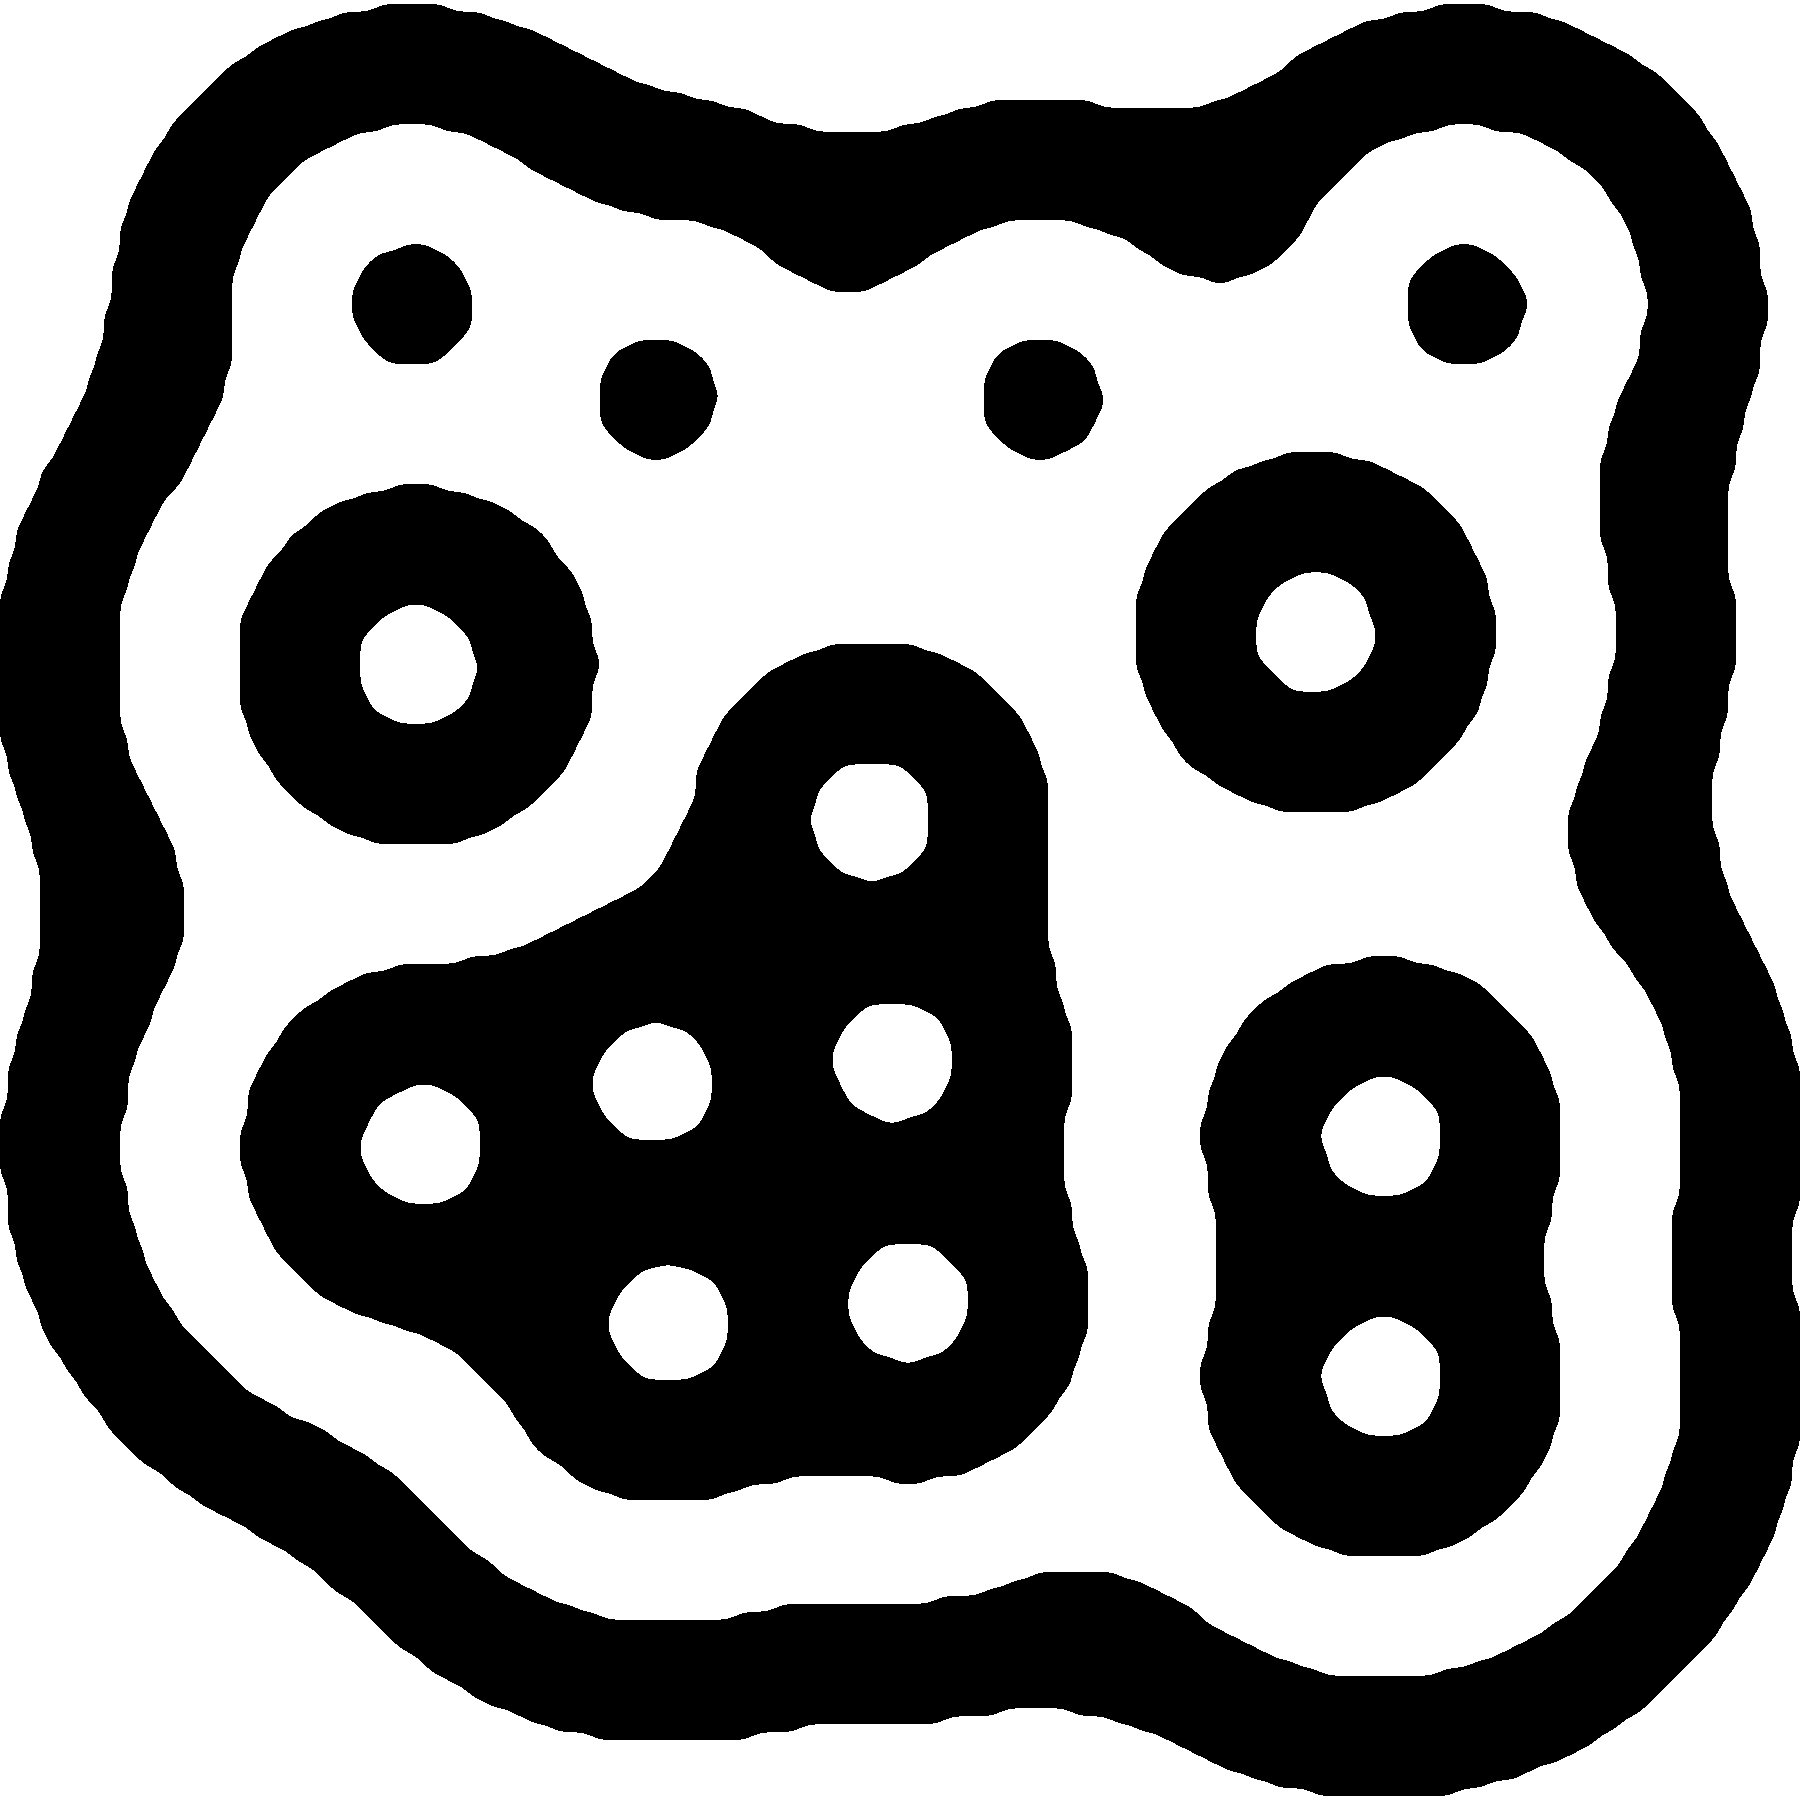
\includegraphics[height=1in]{img/ImplementierungInput/ReactivisionCode.png}
	\caption{ReacTIVision Code}
	\label{fig:img_ImplementierungInput_ReactivisionCode}
\end{figure}

Die ReacTIVision-Software ist plattformübergreifend für Windows, Linux und Mac OS X verfügbar. Sie greift über plattformspezifische Schnittstellen auf angeschlossene Kamera zu und wertet das empfangene Bild in Echtzeit aus. Dabei sind bei einer Kameraauflösung von 1024 x 68 Bildpunkten Bildraten von 15-20 Bildern pro Sekunde erreichbar. Diese Leistung wird auch durch eine höhere Anzahl von gleichzeitig im Bild vorhandenen Codes nicht merklich geringer.

Neben der Position der Codes wird auch deren aktuelle Rotation sowie die erste Ableitung dieser drei Parameter (also ein Maß für die Bewegung) extrahiert. Zudem können Finger, die die Oberfläche berühren erkannt und deren Position extrahiert werden. Dies ist auch für mehrere Finger möglich, wobei eine eindeutige Zuordnung über die Zeit erhalten bleibt und so rudimentäre Multitouch-Funktionen umgesetzt werden können.

Als problematisch stellt sich wie auch bei allen anderen betrachteten optischen Ansätzen die Abhängigkeit der Erkennungsqualität von der Umgebungsbeleuchtung bzw. deren Änderung dar. ReacTIVision arbeitet mit adaptiven Filteralgorithmen zur Aufbereitung des Bildes, was jedoch nur leichte Beleuchtungsschwankungen ausgleichen kann. Die Software kann händisch an die Beleuchtungsverhältnisse angepasst werden (Einstellung der Blendenöffnung und der Bildverstärkung), bei sich ändernden Lichtverhältnissen muss jedoch regelmäßig eine manuelle Nachführung der Parameter vorgenommen werden.

Die aus dem Bilderstrom gewonnenen Daten werden im Falle einer Änderung zumindest eines Wertes über ein Netzwerkschnittstelle (UDP-basiert) in einem propritären Protokoll zur Verfügung gestellt. Zu diesem Protokoll werden Schnittstellen und Referenzimplementierungen in unterschiedlichen Programmiersprachen, unter anderem C(++) und Java, zur Verfügung gestellt. Applikationen können diese Schnittstelle implementieren und werden sie mittels insgesamt sechs zu implementierenden Methoden an die Erkennungsroutinen angebunden (3 für Code- und 3 für Fingertracking).

% paragraph reactivision (end)

% subsubsection frameworks_für_video_basierten_input (end)

% subsection verfügbare_frameworks (end)

\subsection{Technologieentscheidung} % (fold)
\label{sub:technologieentscheidung}

Auf Basis der Anforderungen, die im Anwendungsfall an das Werkzeug gestellt werden, ist nun nach der grundsätzlichen Entscheidung für ein auf optischen Ansätzen basierenden System die Entscheidung für ein konkretes Framework zu treffen. 

\subsubsection{Vergleich der Frameworks für videobasieren Input}\label{subs:vergleich_video_frameworks}

Für die Anbindung von videobasiertem Input wurde drei Frameworks vorgestellt. Diese Frameworks sind nun hinsichtlich mehrere Aspekte zu vergleichen, die sich aus den Anforderungen der zu erstellenden Applikation sowie der Forderung nach möglichst einfacher (im Sinne von unaufwändiger) Einbindung des Frameworks ergeben. Im Einzelnen sind dies 
\begin{itemize}
	\item die Unterstützung bei der Einbindung von Kameras, eine Schnittstelle zur Programmiersprache Java,
	\item eine stabile und in Echtzeit ablaufende Bilderkennung,
	\item eine ausreichende Anzahl von Codes (Größenordnung 100),
	\item die Extraktion von Position und Rotationsinformation für Codes im Erfassungsbereich der Kamera sowie
	\item die technische und lizenzrechtliche Möglichkeit, die Frameworks an die eigenen Anforderungen anzupassen.
\end{itemize}
    
ReacTIVision bietet die umfassendste Unterstützung zur Einbindung unterschiedlicher Videoquellen und ist zur Anwendungsseite hin durch die Netzwerkschnittstelle am flexibelsten einsetzbar. Alle drei Ansätze bieten Schnittstellen bzw. Konnektoren für die Programmiersprache Java an. Die Frameworks selbst sind in C(++) oder Java erstellt und können auf den gängigen Plattformen (Windows, Linux, Mac OS x) ausgeführt werden. Eine Verteilung der Applikation auf mehrere Rechner wird nur von ReacTIVision explizit unterstützt.

Hinsichtlich der eigentlichen Bilderkennungs-Routinen sind die Ansätze in ihrer Leistung und Geschwindigkeit vergleichbar, leiden aber alle unter der Abhängigkeit von der Umgebungsbeleuchtung. ReacTIVision bietet hier als einziger Ansatz die Möglichkeit, Kameraparameter zur Laufzeit nachzuführen und so Schwankungen der Umgebungshelligkeit auszugleichen.

Durch den eingesetzten Mapping-Ansatz sind ARToolkit und ReacTIVision hinsichtlich Form und Inhalt der Codes flexibler als direkt codierende Ansätze wie Visual Codes. Dies ist im konkreten Anwendungsfall relevant, da aufgrund der Token-Form und deren beschränkter Größe eine ideale Platzausnutzung erfolgen muss, um ausreichende Erkennungsleistung zu gewährleisten.

Die Extraktion der Raumparameter (Neigungsinformation, ...), die von ARToolkit und Visual Codes ermöglicht wird, ist in bei tisch-basierten Werkzeugen wie dem hier vorgestellten nicht notwendig - die Erhebung planarer Parameter (Position und Rotation) ist ausreichend.

Die Anzahl der verfügbaren und zuverlässig unterscheidbaren Codes muss für die hier vorgeschlagene Anwendung in der Größenordnung 100 liegen. Visual Codes und ReacTIVision erfüllen diese Anforderung, ARToolkit bietet im Lieferumfang weniger Codes an, diese können jedoch erweitert werden und bieten auch in der gerforderten Anzahl noch ausreichend Unterscheidungsmerkmale für eine zuverlässige Unterscheidung (REF Schmalstieg TU System).

Von allen drei Systemen steht der Source-Code zur Verfüng. Lizenzrechtlich erlauben ebenfalls alle Systeme eine Veränderung des Sourcecode (LIZENZEN AUFZÄHLEN)

\begin{center}
	\begin{tabular}{| p{3cm} || p{3cm} | p{3cm} | p{3cm} |} \hline
		 & ARToolkit & Visual Codes & ReacTIVision \\ \hline \hline
		Kamera\-unterstützung 		  		& ? & nativ nur für Mobiltelefone & nativ auf allen unterstützten Plattformen via USB und Firewire \\ \hline
		Plattformen 			  	  		& x & Java-basiert auf allen Plattformen & Windows, Linux, Mac OS X \\ \hline
		Schnittstelle zu Java 		  		& ja & ja & ja \\ \hline
		Stabilität der Bilderkennung 	  	& eher hoch & eher hoch & hoch \\ \hline
		Geschwindigkeit der Bilderkennung 	& > 10 fps & > 10 fps & > 10 fps \\ \hline
		Anzahl von Codes 		  			& eher hoch & hoch & hoch \\ \hline
		Erkennung von Position 		  		& ja & ja & ja \\ \hline
		Erkennung von Rotation 				& ja & ja & ja \\ \hline
		Source-Code verfügbar 			  	& ja & ja & ja \\ \hline
		Lizenz 				 				& ? & ? & ? \\ \hline
	\end{tabular}
\end{center}

Auf Basis dieses Vergleichs ist erkennbar, dass das ReacTIVision-Framework für den hier verfolgten Ansatz am besten geeignet erscheint. Es wird deshalb zur Umsetzung des Werkzeugs verwendet. Der zusätzliche Einsatz eines generischen Frameworks zur Flexibilisierung der Applikationsstruktur ist damit nach wie vor möglich und wird im nächsten Abschnitt diskutiert.

% subsubsection vergleich_video_frameworks (end)

\subsubsection{Vergleich der generischen Frameworks}\label{subs:vergleich_generische_frameworks}

Der Einsatz eines generischen Frameworks ist im konkreten Anwendungsfall für die Modularisierung der Interpretations- und Output-Module denkbar. Eine weitere Anwendung von generischen Frameworks ist die Anforderung nach der Skalierbarkeit der Anzahl der Ausgabemodule ggf. auch während des Betriebs der Applikation (um z.B. weitere Viewer-Module zur Beobachung des Modellierungsvorganges während der Laufzeit zuschalten zu können). Die Aspekte die beim Vergleich der vorgestellten Ansätze berücksichtigt werden müssen, sind deshalb
\begin{itemize}
  	\item die Unterstützung von modularen funktionalen Einheiten sowie
	\item die Möglichkeit diese zur Laufzeit zu laden und entfernen und
	\item die Konfigurierbarkeit der Verknüpfungen dieser Module.
	\item Daneben sind nicht-funktionale Anforderungen wie Skalierbarkeit und
	\item Effizienz bei der Weiterleitung und Verteilung der Anwendungsdaten 
\end{itemize}  
zu berücksichtigen.

Die Modularisierung der Applikation wird von allen vier vorgestellten Frameworks unterstützt. Das Context Toolkit, Papiermaché und TUIpist unterscheiden dabei konzeptuell zwischen unterschiedlichen Arten von von Modulen (im Wesentlichen "Input", "Verarbeitung" und "Output"), das SiLiCon Context Framework unterscheidet nicht zwischen unterschiedlichen Modultypen, dort wird die Rolle eines Moduls ausschließlich über seine Attribute (also die nach außen sichtbaren funktionalen Einheiten) definiert.

Eine Erweiterbarkeit der Applikation zur Laufzeit ist nur beim SiLiCon Context Framework und bei TUIpist möglich. DAs SiLiCon Context Framework arbeitet hier mit eigens erstellten Java-Classloadern, die das Nachladen von Klassen (Modulen) und deren Integration in die Infrasturktur erlauben. TUIpist verwendet die inhärent dynamische Erweiterbarkeit des Java Jini (REF) Frameworks, auf Basis dessen es implementiert wurde. Das Context Toolkit und Papiermaché erlauben kein Nachladen oder Entfernen funktionaler Einheiten während der Laufzeit.

Die Konfiguration der Verbindungen zwischen den Modulen ist bei allen Frameworks möglich, konzeptuell jedoch unterschiedlich ausgeführt. Im Context Toolkit und in Papiermaché muss die Verbindung direkt im Programmcode codiert werden und wird im wesentlichen auf Methodenaufrufe abgebildet. Das SiLiCon Context Framework verwendet ereignisbasierte Regeln, um Module zu verknüpfen. Ein von einem Modul ausgelöstes Ereignis kann hier (ggf. durch Bedingungen eingeschränkt) Aktionen in anderen Modulen auslösen. Eine Besonderheit dieses Ansatzes ist, das Teile der Interpretationslogik (also der Erkennung von Benutzerinteraktion aus den Rohdaten) in die Regeln ausgelagert werden und damit jederzeit dynamisch verändert werden können. So kann zum Beispiel die Interpretation der Nähe zwischen zwei Token in einer Regel codiert werden und so in die Reihe der zulässigen (bzw. erkennbaren) Interaktionen aufgenommen werden. TUIpist benötigt hingegen keinerlei explizite Verbindung der Module, da sämtliche Koordination über den geteilten Datenraum ausgeführt wird. Die Verknüpfungslogik wird hier in die Module verschoben, die selbst wissen müssen, für welche Daten für sie ggf. relevant sind und welche sie deshalb dem Tuplespace entnehmen.

Hinsichtlich der Skalierbarkeit der Frameworks können aufgrund mangelnder Vergleichsdaten keine fundierten Aussagen getroffen werden. Hinzuweisen ist jedoch auf die Unterstützung von verteiltem Betrieb einer Applikation durch das SiLiCon Context Framework (via SOAP-Aufrufe (REF) und das TUIpist Framework (via Jini und Java RMI (REF)). Durch diese Verteilbarkeit ist kann die Problematik mangelnder Rechenressource umgangen werden, die vorallem bei rechenintensiven Anwendungen wie der eingesetzten Bildanalyse im optischen Tracking auftritt.

Die Beurteilung der Effizienz der Frameworks ist hier in Hinblick auf die geforderte Echtzeit-Interaktion mit dem System als relevant zu erachten. Das Haupt-Kriterium für Effizienz ist dementsprechend die Verzögerung zwischen Eingabe-Ereignissen und dem Feedback auf Applikationsebene, die beim Einsatz der Frameworks auftritt. Eine Beurteilung in absoluten Zahlen kann hier mangels entsprechenden Datenquellen ebenfalls nicht erfolgen, konzeptuell sind aber bei den Frameworks, in denen Module direkt durch Programm-Code verknüpft werden (Context Toolkit und Papiermaché), eher geringe Verzögerungen zu erwarte. Die beiden Frameworks, die mit expliziter und konfigurierbarer Middleware zur Datenvermittlung arbeiten (SiLiCon Context Framework und TUIpist) lassen eher höhere Verzögerungen erwarten, wobei der ereignisbasierte Ansatz des SiLiCon Context Framework dem daten-basieren Ansatz von TUIpist insofern überlegen ist, als das bei der datenbasierten Interaktion die Module in regelmäßigen Intervallen nach neuen Daten suchen müssen (Polling, Information Pull-Ansatz), während bei ereignisbasierten Ansätzen die Benachrichtung der betroffenen Module automatisch und zum Zeitpunkt des Auftretens des Ereignisses erfolgt (Information Push-Ansatz). Der Information Pull-Ansatz sorgt dabei einerseits für erhöhten Kommunikationsaufwand und potentiell für Verzögerungen bei Ereignissen, die innerhalb eines Polling-Intervalls auftreten.

-- VERGLEICHSTABELLE --

Auf Basis dieser Gegenüberstellung erscheinen das SiLiCon Context Framework und TUIpist als die beiden geeignetsten Kandidaten für den Einsatz als generisches Framework im hier vorgestellten Anwendungsfall. Das Context Toolkit und Papiermaché scheiden aus verschiedenen Gründen, vorallem aber der mangelnden Flexiblität aus.

Stellt man die beiden verbleibenden Frameworks gegenüber, so sind hinsichtlich der funktionalen Anforderungen keine Vorteile für einen der beiden Kandidaten zu identifizieren. Hinsichtlich der nichtfunktionalen Anforderungen scheint TUIpist hinsichtlich der Skalierbarkeit leichte Vorteile zu haben, da das Nachladen von neuen Instanzen weniger Aufwand versacht als im Fall des SiLiCon Context Framework (lediglich Laden eines Moduls im ersten Fall gegenüber Laden und Einbinden über eine Änderung der Regelbasis im zweiten Fall). Außerdem ist die technologische Basis der Verteilungsarchitektur in TUIpist konzeptionell auf höherer Ebene angesiedelt und mächtiger in der Verwaltung der Applikationsstruktur (unter anderem werden neue Module bei TUIpist automatisch in die Infrastruktur eingebunden, sobald sie angemeldet werden, im SiLiCon Context Framework muss für jeden Kommunikationskanal die IP-Adresse des Empfängers bekannt sein und in die Regelbasis aufgenommen werden). 

Hinsichtlich der Effizienz der Kommunikation bietet das SiLiCon Context Framework gegenüber TUIpist aus den oben beschriebenen Gründen (Benachrichtung über Änderungen gegenüber Polling) Vorteile. Für die hier beschriebene Applikation fällt die Entscheidung trotzdem zugunsten TUIpist. Neben der generell unaufwändigeren Konfigurierbarkeit kommt die Struktur von TUIpist einem iterativen Software-Entwicklungsprozess insofern eher entgegen, als dass die Modularisierung von initialen, monolithischen Prototypen (z.B. basierend auf der Struktur des zuvor ausgewählten ReacTIVision-Frameworks) einfacher möglich ist. Dies liegt darin begründet, dass in der modularen und dynamischen Struktur von TUIpist die gesamte Applikationslogik in den Modulen enthalten ist und so Teile aus einer monolithischen Applikation herausgelöst und direkt übernommen werden können, wobei lediglich die Logik der Datenübergabe von direkten Methoden-Aufrufen auf die TUIpist-Routinen zum Zugriff auf den Tuplespace umgearbeitet bzw. erweitert werden muss. Beim korrekten Einsatz des SiLiCon Context Framework wandert wie oben beschrieben ein Teil der Applikationslogik in die Regelbasis, was erhöhten Aufwand bei der iterativen Entwicklung verursacht und außerdem das Zusammenspiel der Applikations-Module unübersichtlicher und schwerer fassbar macht.

% subsubsection vergleich_generische_frameworks (end)

% subsection technologieentscheidung (end)
% section möglichkeiten_zur_erfassung_von_benutzerinteraktion (end)

\section{Konzeption und Umsetzung der Hardwarekomponenten} % (fold)
\label{sec:konzeption_und_umsetzung_der_hardwarekomponenten}

Basierend auf der oben getroffenen Techhnologieentscheidung zugunsten eines optischen, video-basierten Input-Systems für das hier zu erstellende Tabletop Interface wird in diesem Abschnitt das konkrete Hardware-Design beschrieben. Dies umfasst die Beschreibung des Tabletop Interfaces im Überblick und detaillierte Betrachtungen des Token-Designs sowie der Tisch-Oberfläche, die als Input-Kanal dient. Im weiteren werden spezifische Herausforderungen und der jeweilige hier verfolgte Lösungsansatz beschrieben. Nicht Gegenstand dieses Abschnitts sind jene Hardware-Komponenten, die für die Ausgabe von Information eingesetzt werden. Obwohl hier im Überblick angeführt, werden sie detailliert erst in Kapitel XY über die Visualisierung der Modellierungsinformation beschrieben.

\subsection{Überblick} % (fold)
\label{sub:Überblick}

Das Tabletop Interface ist als Tisch mit einer Oberfläche von 100 cm x 80 cm ausgeführt. Die Höhe beträgt 110 cm. Die wesentlichen Hardwarekomponenten sind die Tischoberfläche, die in semi-transparenten Acrylglas ausgeführt ist und die Bodenplatte, in die die Kamera zum optischen Tracking der Tokens auf der Oberfläche sowie der Videoprojektor zur Ausgabe von Information auf der Oberfläche (Projektion von unten) eingebaut sind (siehe Abbildung \ref{fig:img_ImplementierungInput_TischSeitenansicht}). Der Tisch ist auf allen Seitenflächen mit Platten aus Styropor (MARKENNAME -> KUNSTSTOFF) verkleidet, um im Inneren kontrollierte Umgebungslichtbedingungen für die Bilderfassung mit der Kamera zu schaffen. Die kontrollierten Bedingungen werden durch den Einsatz von vier Beleutungsmodulen gewährleistet, die ebenfalls in der Bodenplatte integriert sind und über den Seitenflächen eingebaute Streuscheiben für eine einheitliche, diffuse Beleuchtung der Tischinnenraums sowie der Oberfläche sorgen.

\begin{figure}[htbp]
	\centering
		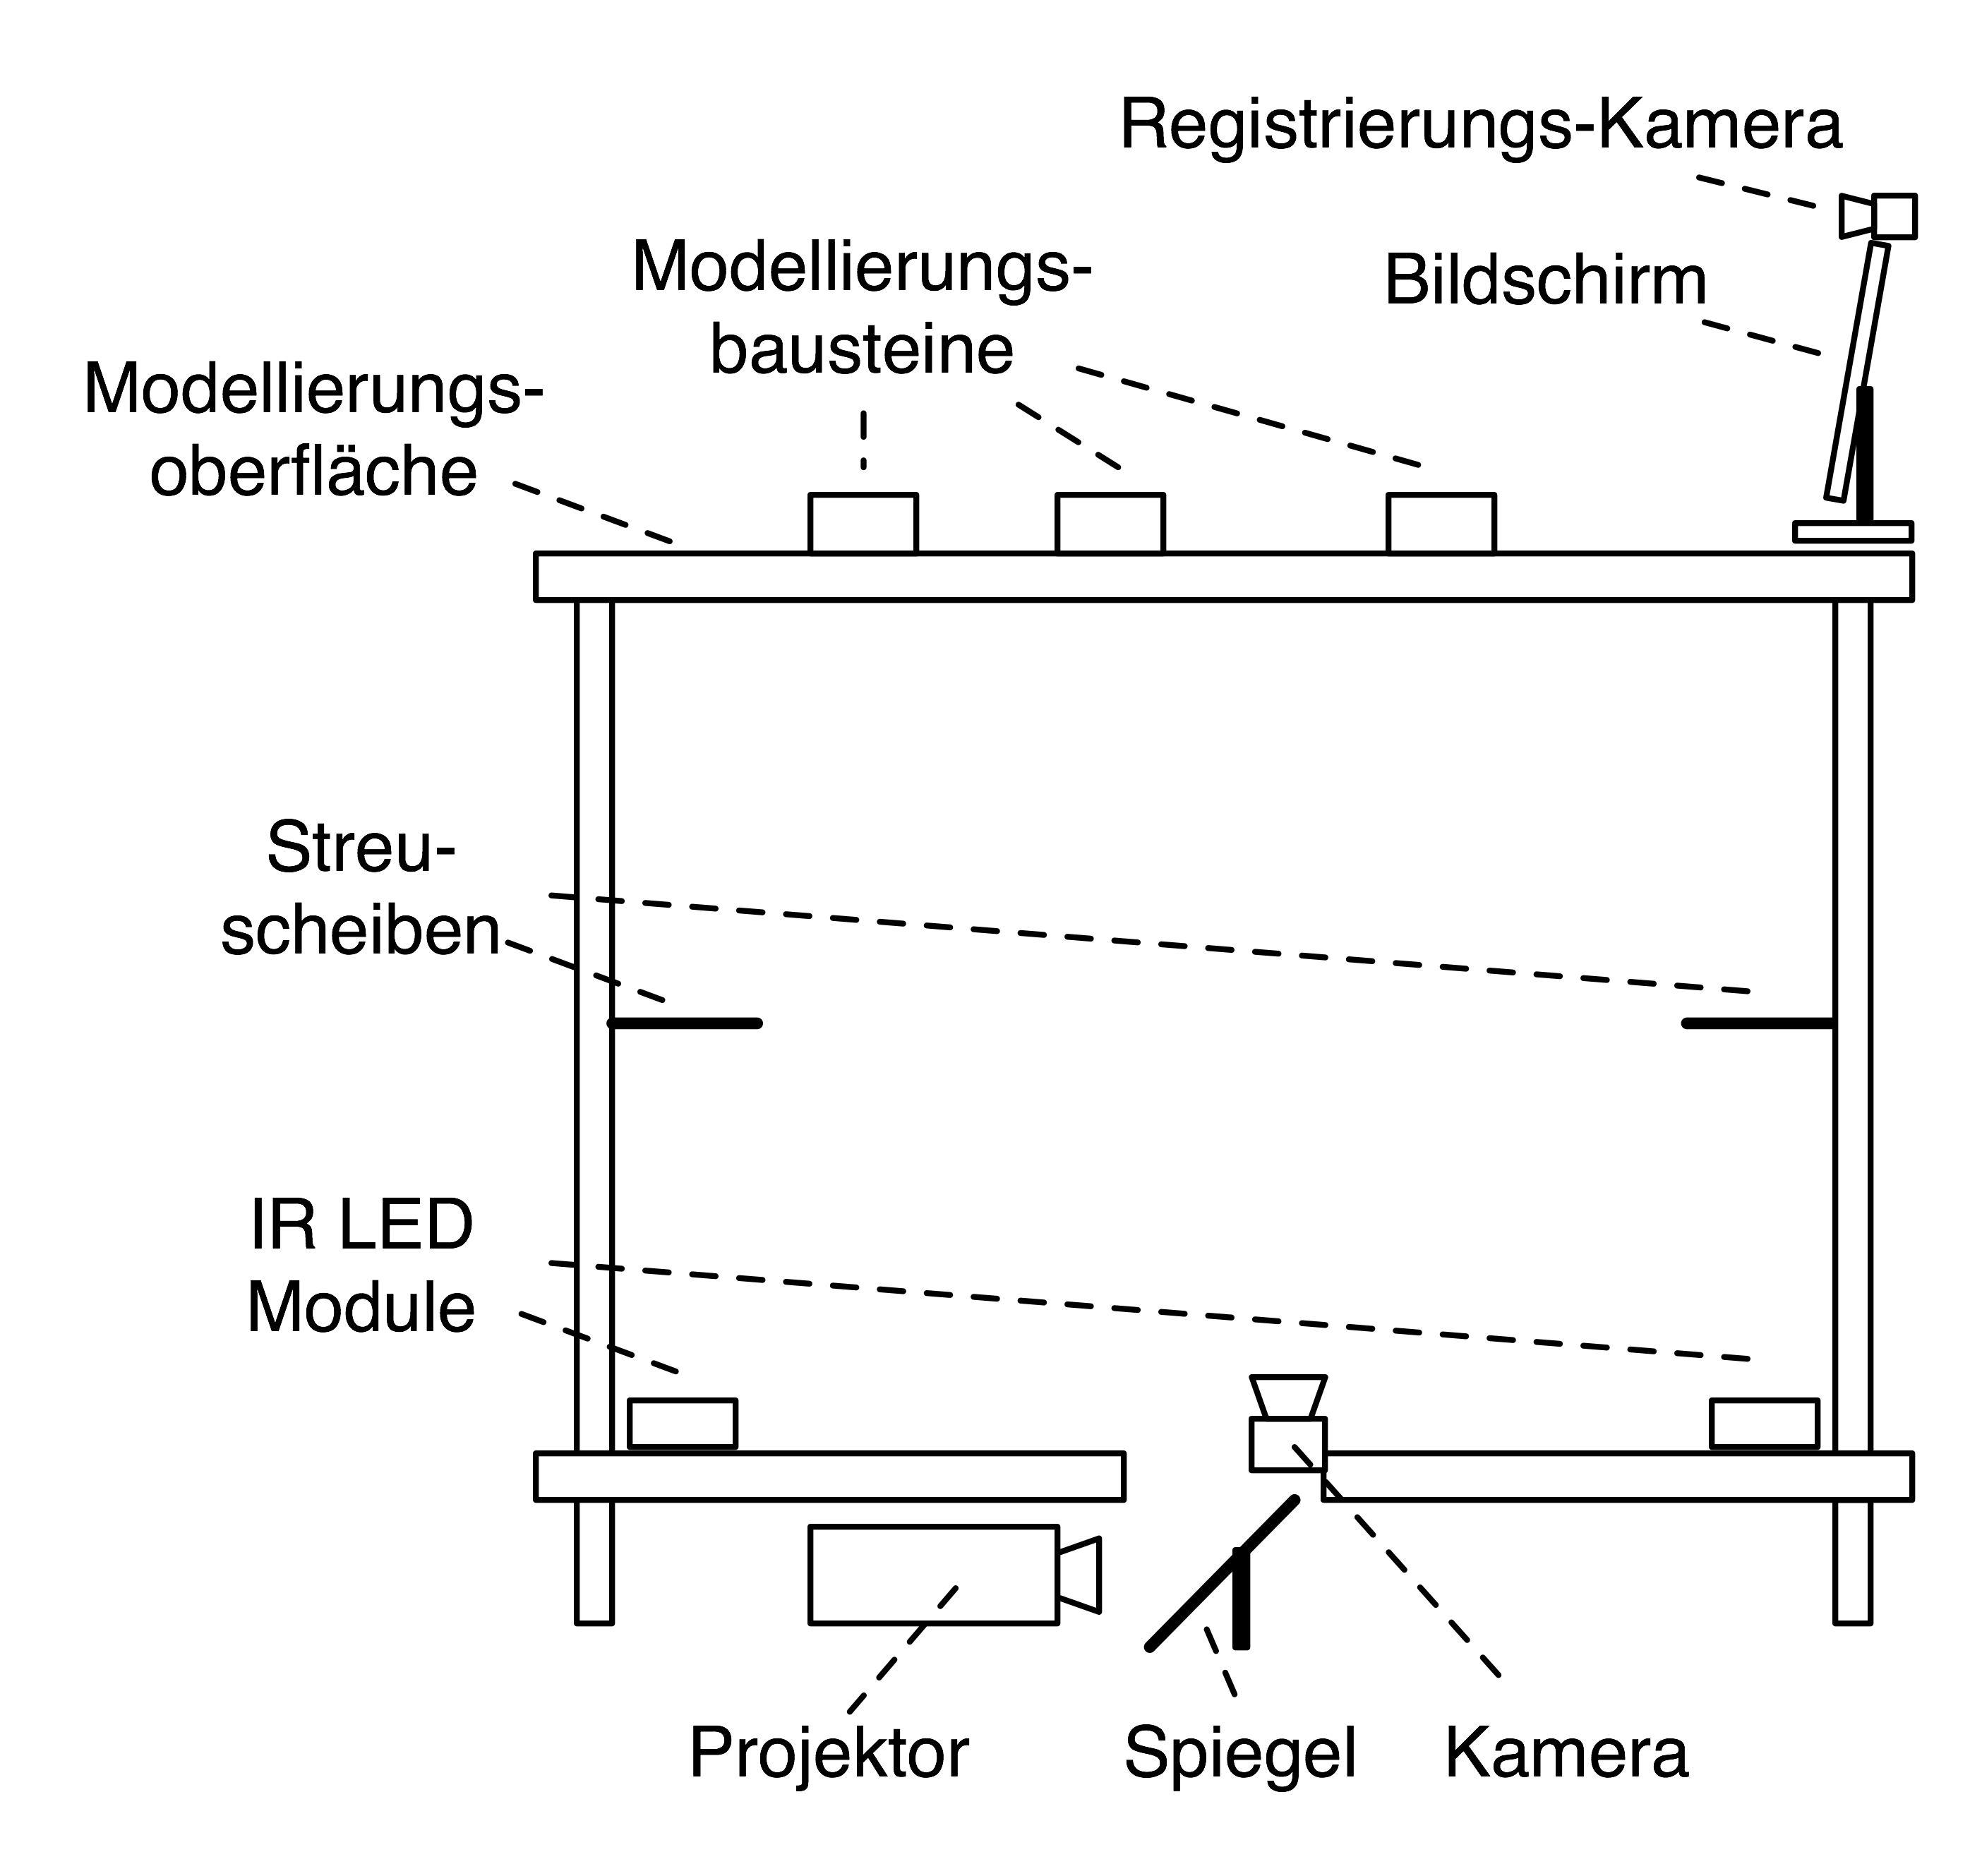
\includegraphics[height=4in]{img/ImplementierungInput/TischSeitenansicht.png}
	\caption{Überblick über den Aufbau des Tabletop Interfaces}
	\label{fig:img_ImplementierungInput_TischSeitenansicht}
\end{figure}

Am Tisch befindet sich zusätzlich ein Bildschirm, auf dem entsprechend der Anforderungen zur Unterstützung der Modellierung Zusatzinformation ausgegeben wird. Eine zweite Kamera, die am Bildschirm sitzt und der unterstützenden Erfassung von Information dient (zum Beispiel der Registrierung von geschachtelten Token wie oben bereits beschrieben).

Das gesamte System ist so zerlegbar, dass es im Kofferraum eines Mittelklassewagens transportiert werden kann. Es werden dazu die Verkleidungsplatten und Tischbeine entfernt, die Tischplatte kann dann direkt auf die Bodenplatte gesetzt und verbunden werden. Das Volumen reduziert sich dabei auf 100 cm x 80 cm x 20 cm, wobei die Tischbeine, die Verkleidungsplatten und der Videoprojektor separat transportiert werden müssen. Ein Zusammenbau des Systems inklusive Kalibrierung der Eingabe- und Ausgabe-Kanäle ist in etwa 30 Minuten möglich.

% subsection Überblick (end)

\subsection{Tokens \& Input-Werkzeuge} % (fold)
\label{sub:tokens_&_input_werkzeuge}

In diesem Abschnitt werden die einzelnen durch die Benutzer manipulierbaren Token-Arten beschrieben. Neben den eigentlichen Modellierungstokens sind dies die Tokens zur Einbettung in Container sowie die Werkzeugtokens, von denen es Ausführungen zur Manipulation des Modells und Tokens zur Auslösung bzw. Kontrolle spezifischer Funktionalitäten gibt.

\subsubsection{Modellierungs-Tokens} %fold 
\label{subs:modellierungs_tokens}

Die eingesetzten Modellierungs-Tokens sind aus nicht transparentem Acrylglas gefertigt. Ihre Außenmaße betragen in etwa (je nach Form) 10 cm x 6 cm in der Grundfläche und 4 cm in der Höhe. Damit ist einerseits eine ausreichende Größe zur Anbringung der ReacTIVision-Codes gewährleistet, andererseits sind noch klein genug, um in einer Hand gehalten und manipuliert werden zu können. Die Codes werden auf der Unterseite der Tokens angebracht und auch von unten erfasst (siehe nächster Abschnitt), um eine Verdeckung der Codes während der Manipulation zu verhindern (siehe Abbildung \ref{fig:img_ImplementierungInput_TokensCodes}).

\begin{figure}[htbp]
	\centering
		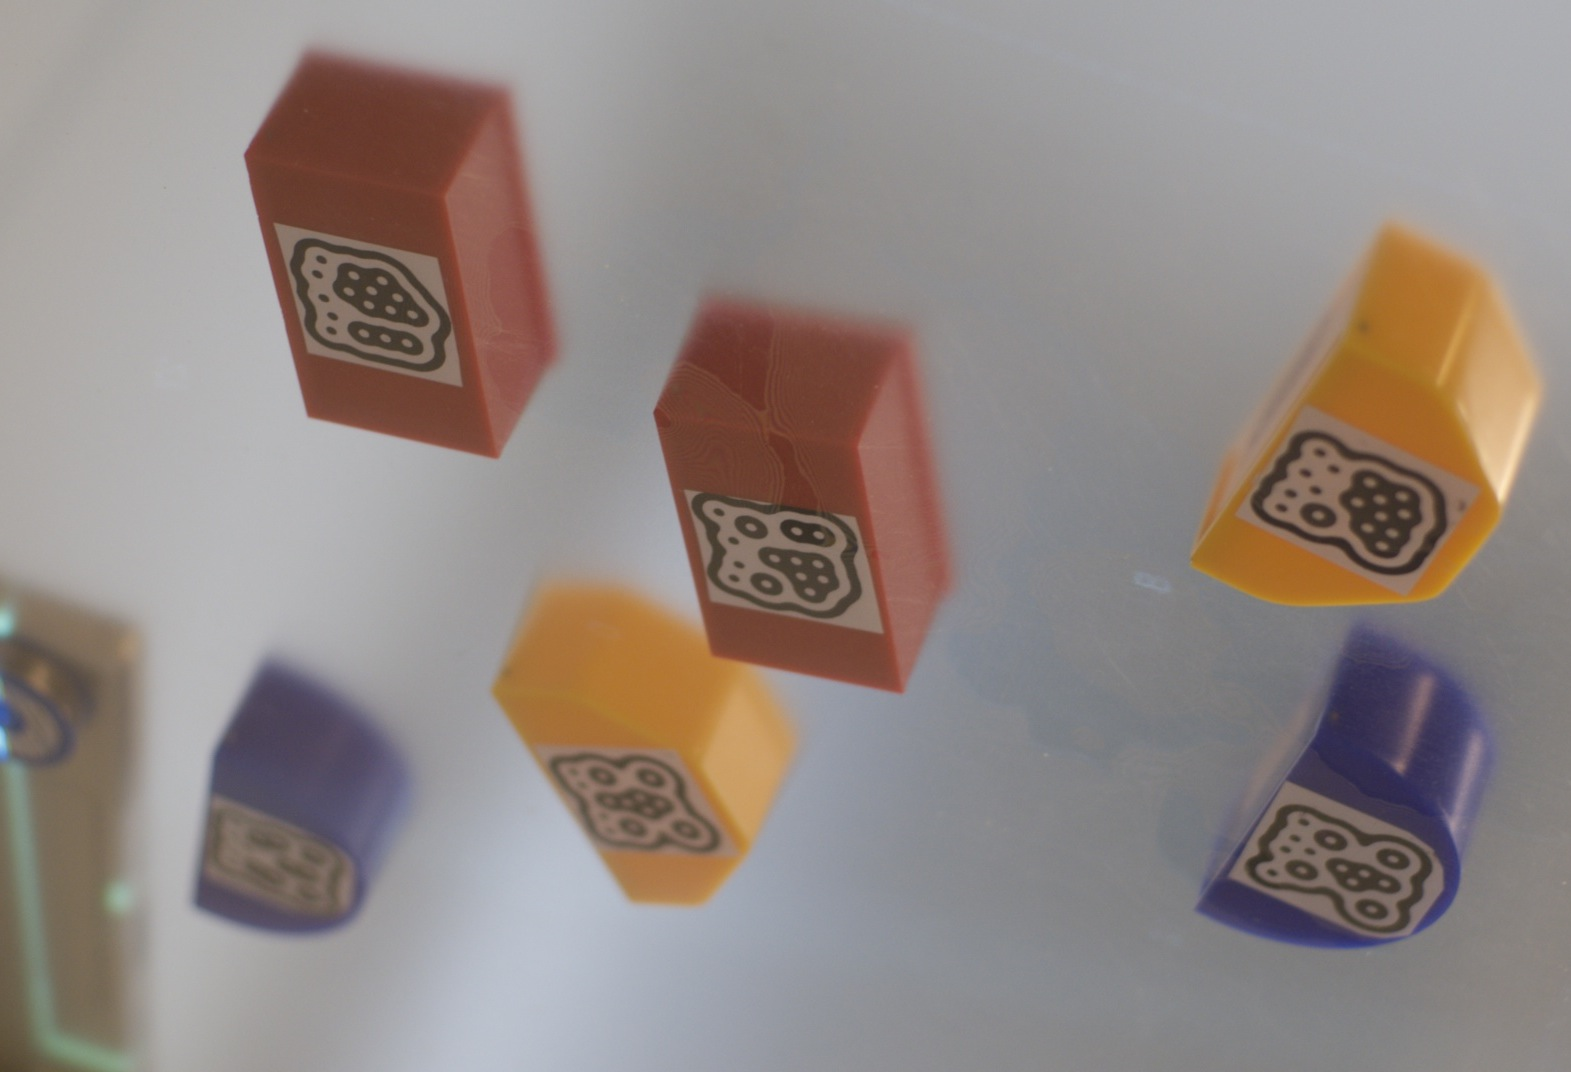
\includegraphics[height=2in]{img/ImplementierungInput/TokensCodes.jpg}
	\caption{An Tokens angebrachte ReacTIVision-Codes zur Identifikation}
	\label{fig:img_ImplementierungInput_TokensCodes}
\end{figure}

\begin{figure}[htbp]
	\centering
		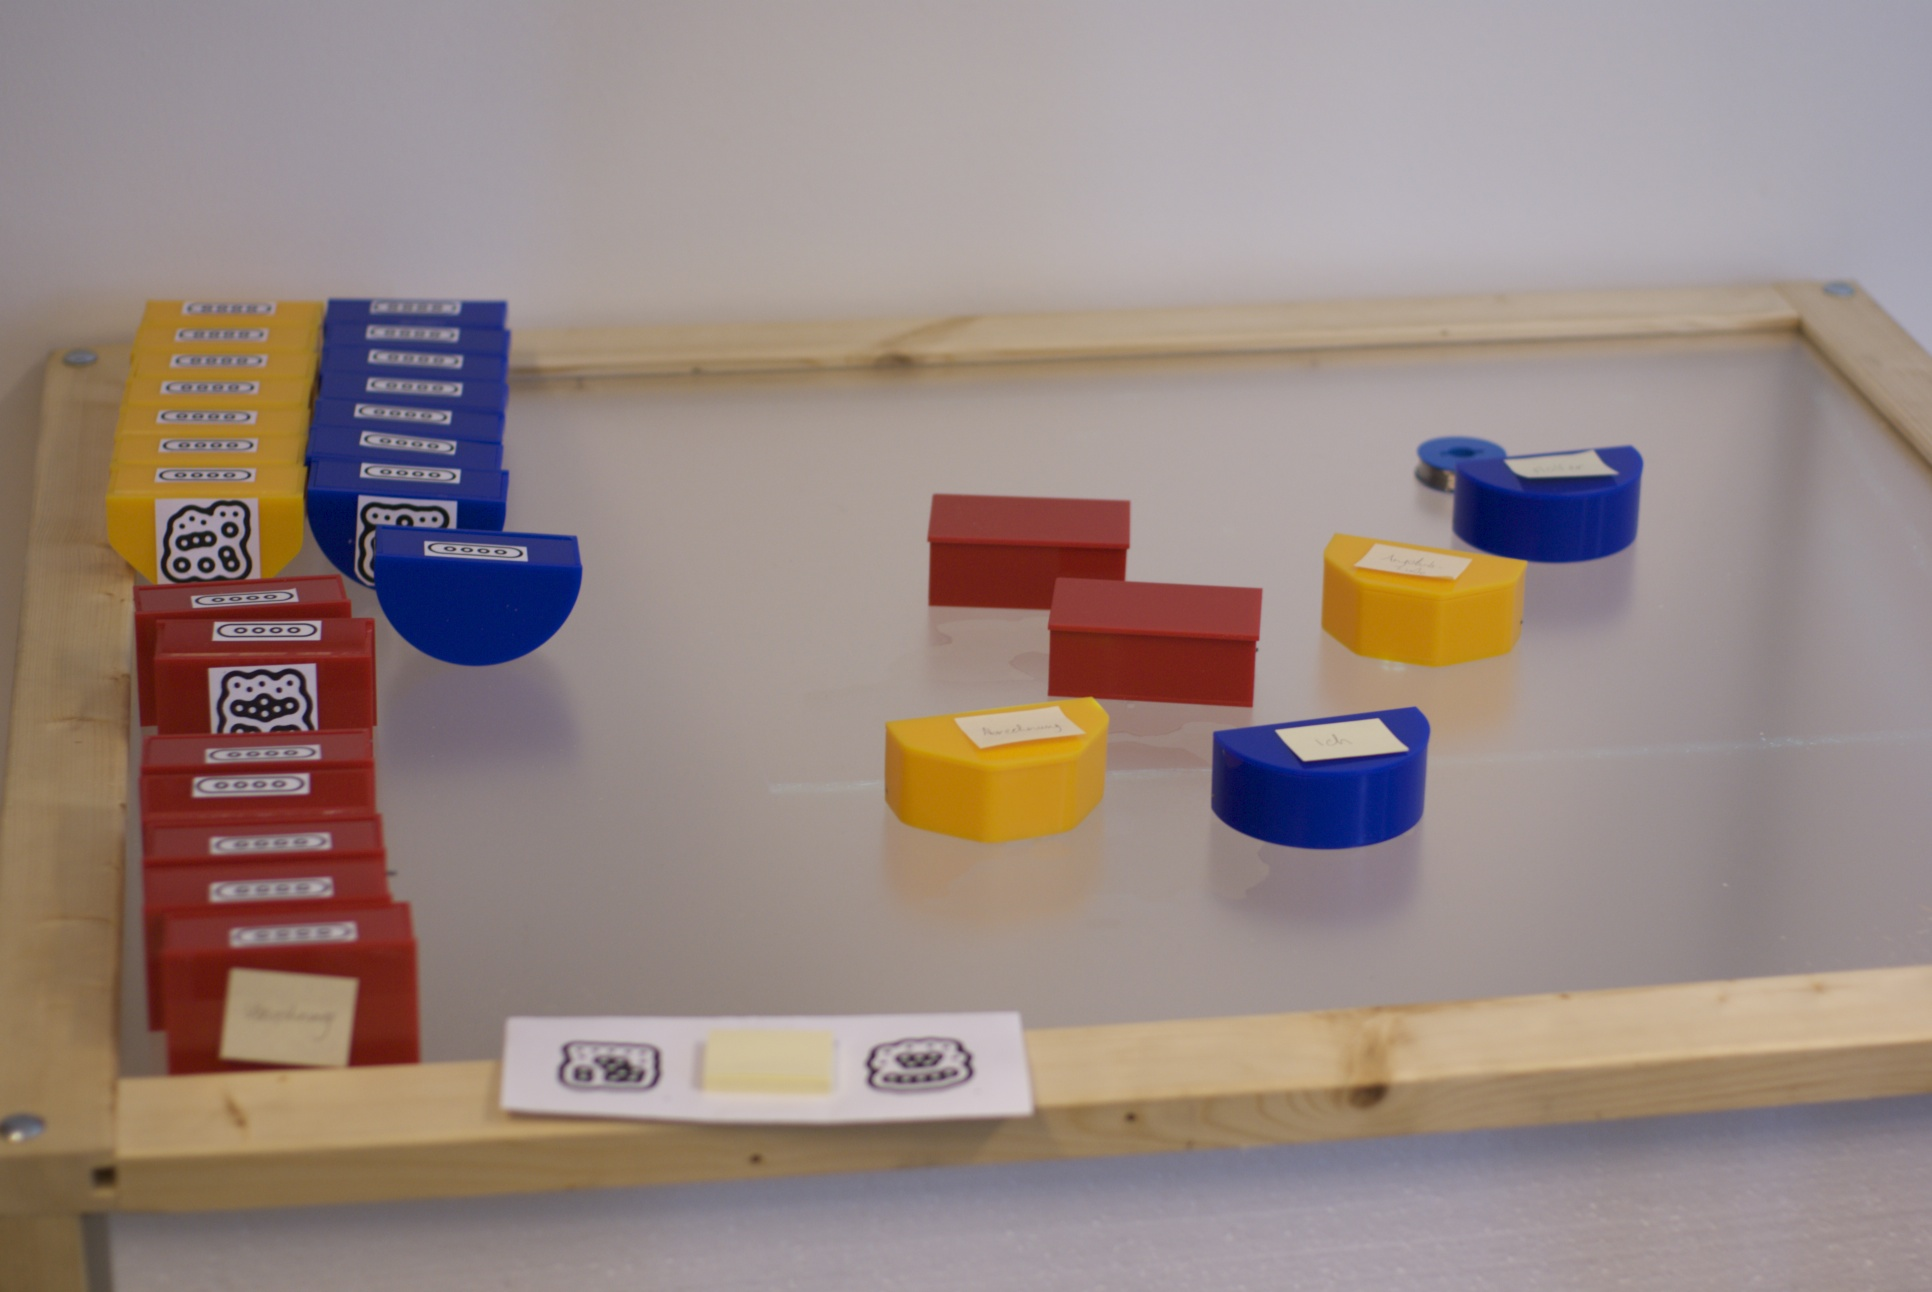
\includegraphics[height=2in]{img/ImplementierungInput/TokenTypes.jpg}
	\caption{Arten von Modellierungstokens}
	\label{fig:img_ImplementierungInput_TokenTypes}
\end{figure}


Die Modellierungs-Tokens wurden in drei Ausführungen gefertigt (siehe Abbildung \ref{fig:img_ImplementierungInput_TokenTypes}). Diese unterscheiden sich in Form und Farbe und können während der Modellierung von den Benutzern frei mit Bedeutung belegt werden. Die Auswahl der Formen und Farben erfolgte inspiriert von den Symbolen gängiger Modellierungsnotationen in Abstimmung mit fertigungstechnischen Einschränkungen. Eine wie in XY (REF von TEI) vorgeschlagene Analyse geeigneter Token-Formen und eine auf diesen Ergebnissen basierende Umsetzung wurde nicht vorgenommen. Die liegt vor allem in der Tatsache begründet, dass sich der Fokus der hier vorgestellten Arbeit im Entwicklungsprozess von einem Werkzeug zur Geschäftsprozessmodellierung (mit vorgegebener Notation) hin zu einem allgemeiner einsetzbaren Werkzeug zur generischen Modellierung konzeptueller Modelle (ohne vorgegebene Notation) entwickelte. Die Auswahl der Token-Formen fiel in die erste Phase, wodurch die Tokens im äußeren Erscheinungsbild an gängige Notationen zur Ablauf-Modellierung angelehnt sind. Die Auswirkung der Token-Form auf die Modellierung scheint aber bei Benutzern ohne Modellierungs-Vorbildung geringen bis keinen Einfluss auf den Modellierungsprozess zu haben (siehe Kapitel XY - Evaluierung).

\begin{figure}[htbp]
	\centering
		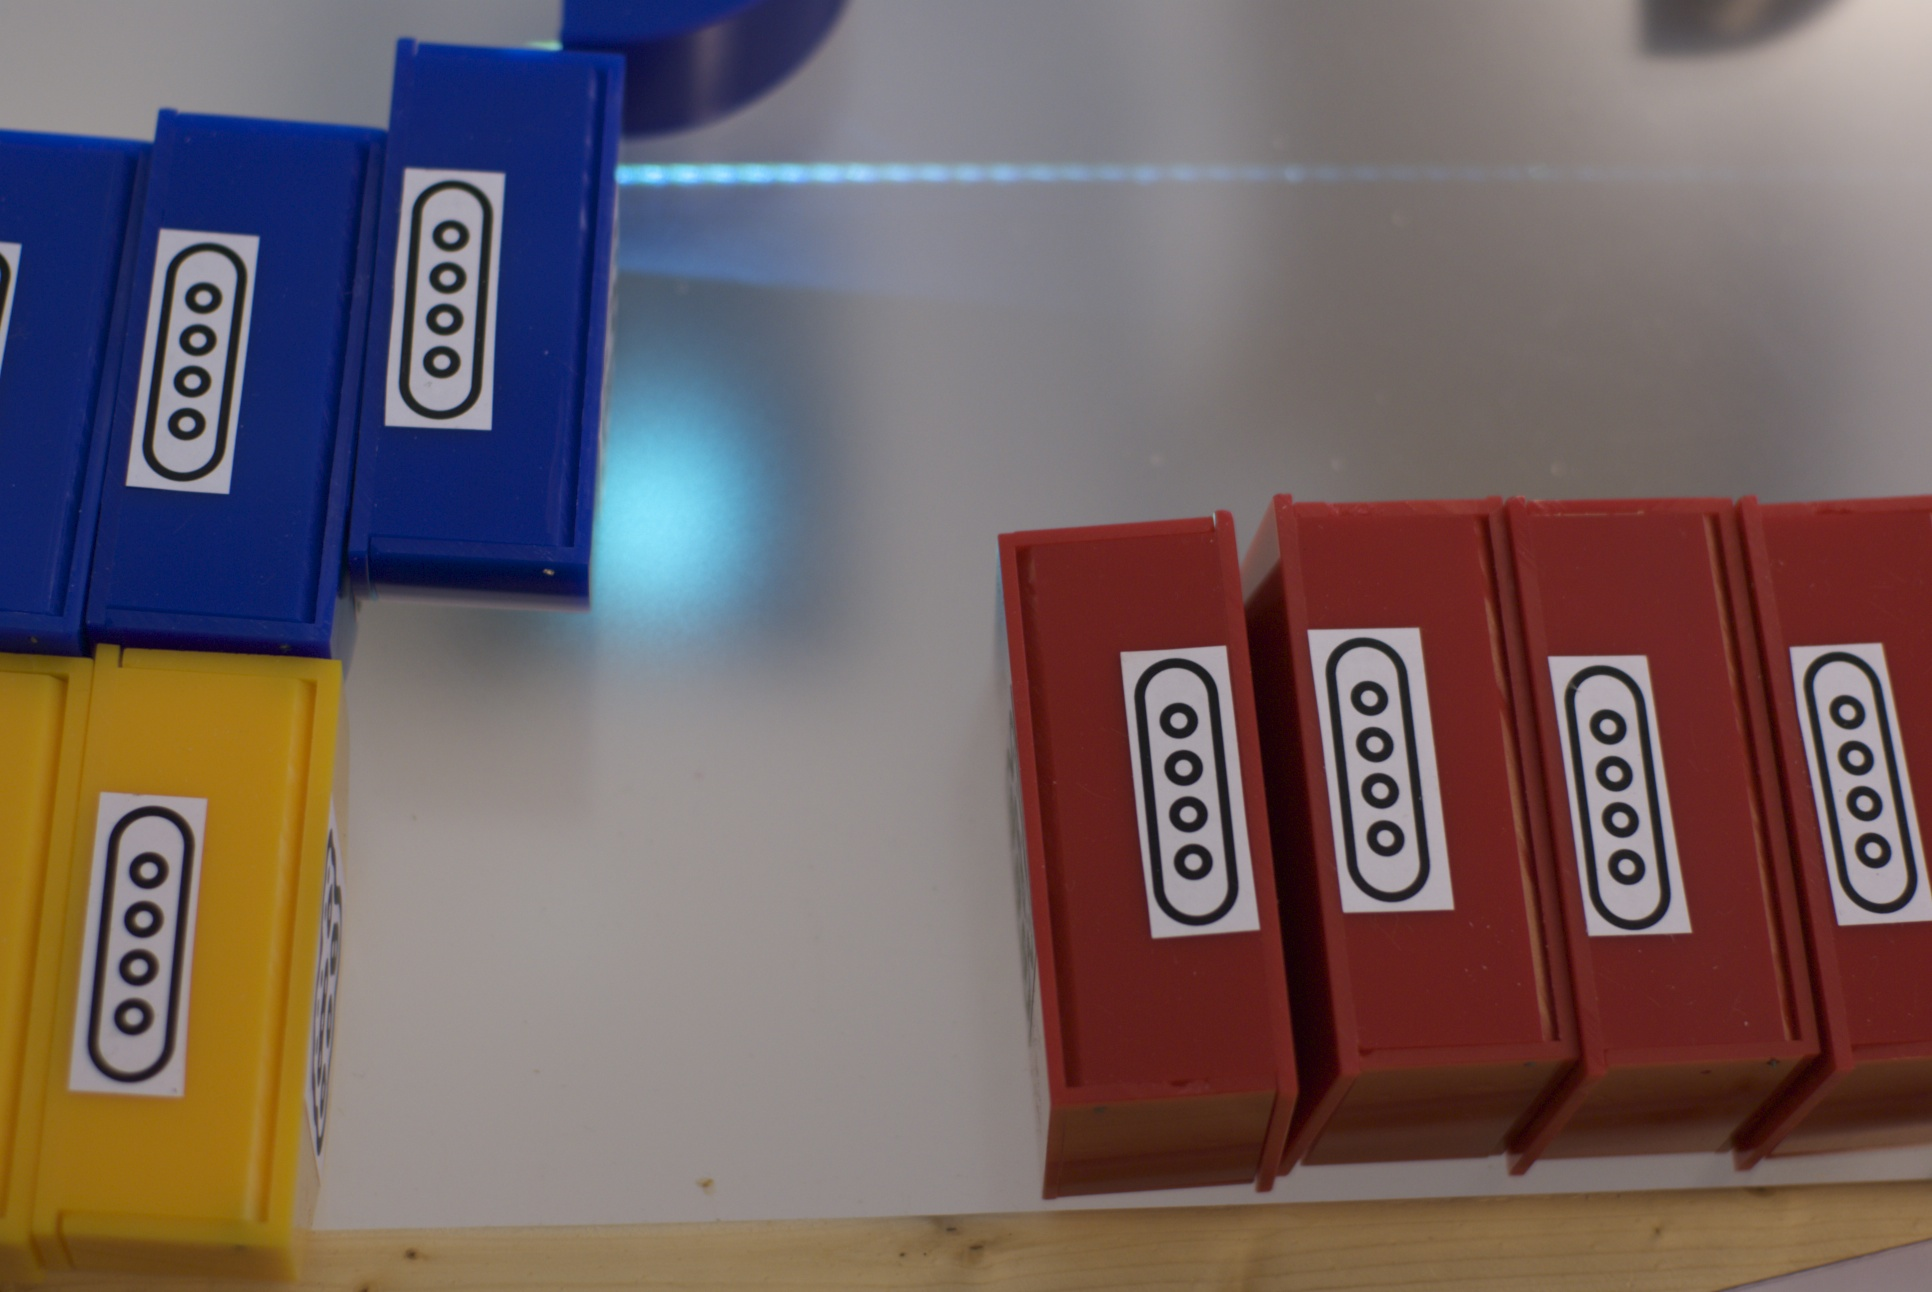
\includegraphics[height=2in]{img/ImplementierungInput/ContainerRueckseite.jpg}
	\caption{Rückwand von Container Tokens}
	\label{fig:img_ImplementierungInput_ContainerRueckseite}
\end{figure}

Wie in der Beschreibung der Anforderungen gefordert und oben bereits beschrieben sind die Modellierungs-Tokens als Container ausgeführt. Im Abschnitt über die Erkennung des Token-Zustands (REF) wurde beschrieben, das beim Einsatz von optischem Tracking eine Möglichkeit geschaffen werden muss, im Kamerabild zu erkennen, ob ein Token geöffnet ist oder nicht. Um den konsequenten Einsatz eines Erkennungsframeworks (ReacTIVision) zu gewährleisten, wird zu diesem Zweck ein zweiter Code eingesetzt (siehe Abbildung \ref{fig:img_ImplementierungInput_ContainerRueckseite}), der nur dann für die Kamera sichtbar wird, wenn das Token geöffnet ist. Hardwareseitig ist dies so umgesetzt, das die Modellierungstokens einen Öffnungsmechanismus besitzen, dessen Schanier nicht am Deckel sitzt (und damit nur diesen beweglich machen würde), sondern an der Bodenplatte, wodurch sich beim Öffnen eines Containers nicht nur der Deckel sondern auch die Hinterwand des Tokens bewegt (siehe Abbildung \ref{fig:img_ImplementierungInput_ContainerToken}). Die Hinterwand kommt im geöffneten Zustand auf der Oberfläche des Tisches zu liegen, wodurch der auf ihr angebrachte zweite Code für die Kamera sichtbar wird. So kann durch das ansich zur Positionsbestimmung eingesetzte optische Trackingsystem zuverlässig auch den Öffnungs-Zustand der Tokens auf der Oberfläche erkennen.

\begin{figure}[htbp]
	\centering
		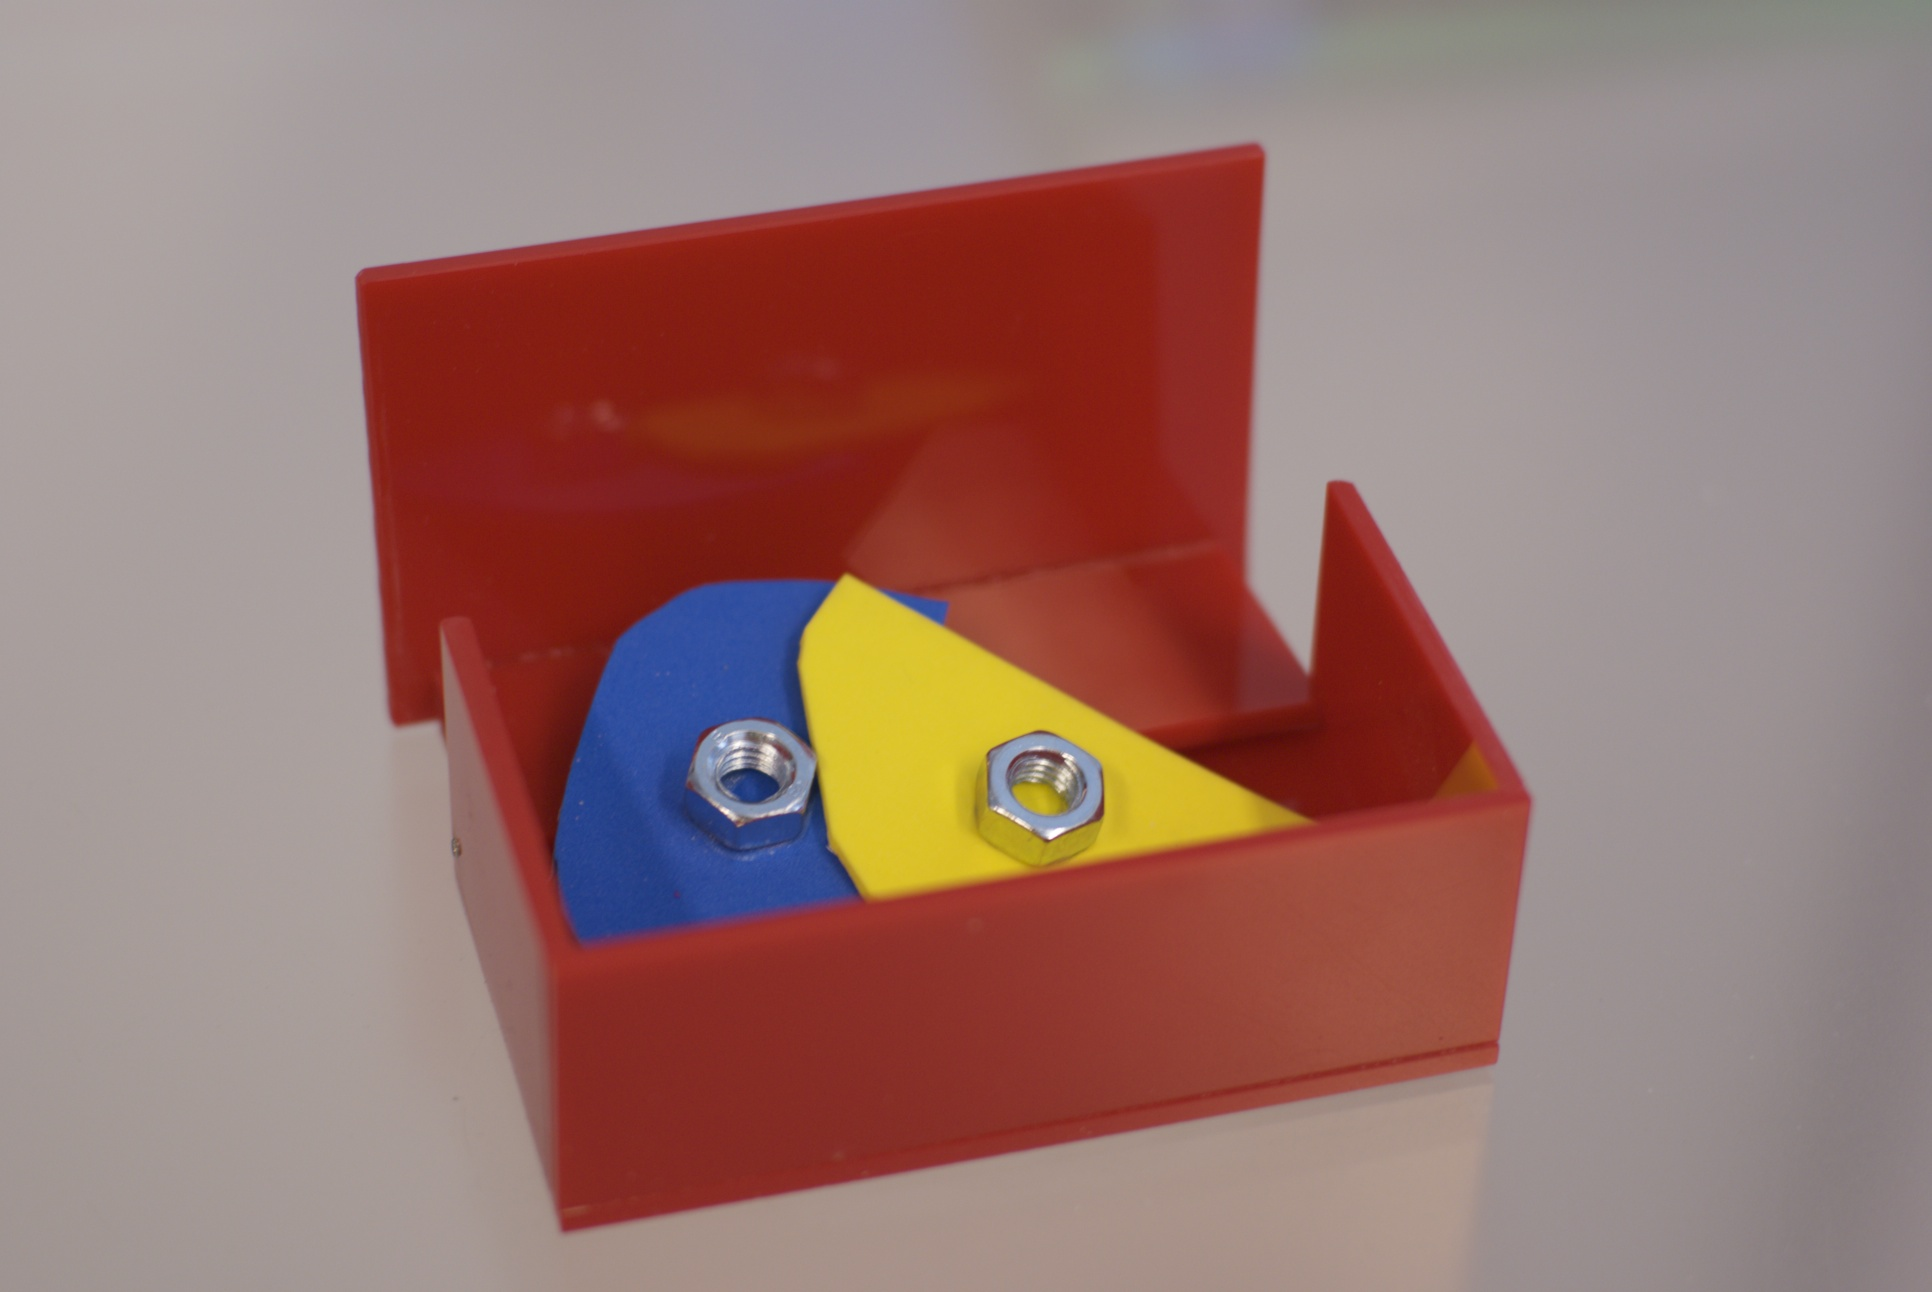
\includegraphics[height=2in]{img/ImplementierungInput/ContainerToken.jpg}
	\caption{Geöffnetes Container Token}
	\label{fig:img_ImplementierungInput_ContainerToken}
\end{figure}

% subsubsection modellierungs_tokens (end)

\subsubsection{Einbettbare Tokens} % (fold)
\label{einbettbare_tokens}

Die einbettbaren Token erlauben wie in Kapitel XY beschrieben die Verschachtelung von Modellen und das Hinzufügen von Zusatzinformation. Sie werden in einem definierten Interaktionsvorgang an Information gebunden und dann in einen Container gelegt. Hinsichtlich des Hardware-Designs sind folgende Anforderungen zu beachten:
\begin{itemize}
	\item Die Token müssen klein genug sein, um auch mehrere Einheiten ein einem Container unterzubringen.
	\item Sie müssen gleichzeitig groß genug sein, um einen ReacTIVision-Code zur eindeutigen Information anzubringen.
	\item Sie müssen so ausgeführt sein, dass haptisch oder akustisch erkennbar ist, ob in einem geschlossenen Container Tokens eingebettet sind oder nicht (z.B. durch Gewicht oder Geräusche beim Schütteln eines Containers).
\end{itemize}

Die einbettbaren Tokens wurden aus flexiblen Kunststoffmatten gefertigt und mit einem Metallstück versehen (siehe Abbildung \ref{fig:img_ImplementierungInput_ContainerToken}), das einerseits als Griff dient und andererseits sowohl das Gewicht erhöht und akustisches Feedback beim Schütteln eines Container-Tokens verursacht. Die einbettbaren Tokens wurden exemplarisch in drei Ausführungen gefertigt, je nach Art und Anzahl der einzubettenden Information kann eine Definition weiterer Tokens sinnvoll sein. Folgende Tokens wurden für den aktuellen Entwicklungsstand des Werkzeugs angefertigt:
\begin{itemize}
	\item Einbettung von Teilmodellen (inhärente Kernfunktionalität des Werkzeugs)
	\item Einbettung von digitalen Ressourcen bzw. Dateien am lokalen Rechner (Erweiterung zur Verknüpfung des Modells mit den realen digitalen Ressourcen aus dem Arbeitskontext)
	\item Einbettung von Fotos (Erweiterung zur Verknüpfung des Modells mit dem realen Arbeitskontext, z.B. mittels Fotos von Arbeitsmitteln oder Personen)
\end{itemize}

Alle Tokens sind auf der Unterseite mit einem ReacTIVision-Code versehen, der sie eindeutig identifiziert. Aufgrund der beschränkten Größe der Tokens ist dieser Code von der Kamera, die die Tischoberfläche erfasst, nur in der Mitte der Oberfläche erfassbar (da dort die geringsten Linsen-Verzerrungen auftreten und der Code somit gerade noch erkannt werden kann). Um etwaige Bedienungsprobleme zu vermeiden, wurde die deshalb die Interaktion mit einbettbaren Tokens (Registrierung, Binden von Information) auf die in Abbildung \ref{fig:img_ImplementierungInput_TischSeitenansicht} dargestellte zweite Kamera ("Registrierungs-Kamera") verlegt, die durch die physische Nähe zu den Modellierenden die Codes der einbettbaren Tokens problemlos erfassen kann.

% subsubsection einbettbare_tokens (end)

\subsubsection{Werkzeug Tokens} % (fold)
\label{ssub:werkzeug_tokens}

Neben den Tokens, die Modellierungsinhalt repräsentieren, wurden auch Tokens angefertigt, der Interaktion mit dem System ansich und der Steuerung der Modellierungsablaufs dienen. Hier sind zwei Arten zu unterscheiden: einerseits gibt es Werkzeuge, die der Manipulation des Modells dienen (z.B. Herstellung von Verbindungen zwischen Tokens, Benennung von Tokens) und andererseits solche, die der Steuerung von modellierungsunterstützender Zusatzfunktionalität dienen (etwa Tokens, die die Rückverfolgung der Modellierungshistorie kontrollieren). Außerdem sind orthogonal zu dieser Klassifizierung noch Tokens zu unterscheiden, die beim Einsatz ein Ereignis auslösen und solche, die die für einen Zustandswechsel des Systems sorgen, solange sie im Einsatz sind (gleich einem Schalter). Im Folgenden werden die einzelnen Werkzeuge beschrieben und den eben definierten Kategorien zugeordnet.

\paragraph{Manipulation des Modellierungsablaufs} % (fold)
\label{par:manipulation_des_modellierungsablaufs}

Die bei der Verwendung des Systems wichtigsten Werkzeug Tokens sind jene, die zur Benennung und Verbindung von Modellierungs-Tokens verwendet werden. 

-- Bild der Auswahl-Werkzeuge --

% paragraph manipulation_des_modellierungsablaufs (end)

\paragraph{Steuerung von Unterstützungsfunktionen} % (fold)
\label{par:steuerung_von_unterstützungsfunktionen}

% paragraph steuerung_von_unterstützungsfunktionen (end)
% subsubsection werkzeug_tokens (end)
% subsection tokens_&_input_werkzeuge (end)

\subsection{Input auf der Tischoberfläche} % (fold)
\label{sub:input_auf_der_tischoberfläche}

Semitransparente Oberfläche, Projektion von unten (Umlenkspiegel), Kamera von unten - Überleitung zur 
Illumination via Interferenz zwischen Beamer und Kamera

\subsubsection{Illumination und Umgebungslichtabhängigkeit} % (fold)
\label{sub:illumination_und_umgebungslichtabhängigkeit}

% subsubsection illumination_und_umgebungslichtabhängigkeit (end)
% subsection input_auf_der_tischoberfläche (end)
% section konzeption_und_umsetzung_der_hardwarekomponenten (end)

\section{Benutzerinteraktion mit dem Werkzeug} % (fold)
\label{sec:benutzerinteraktion_mit_dem_werkzeug}

\subsection{Hinzufügen und Verändern von Modellelementen} % (fold)
\label{sub:hinzufügen_und_verändern_von_modellelementen}

% subsection hinzufügen_und_verändern_von_modellelementen (end)

\subsection{Benennen von Modellelementen} % (fold)
\label{sub:benennen_von_modellelementen}

% subsection benennen_von_modellelementen (end)

\subsection{Verbinden von Modellelementen} % (fold)
\label{sub:verbinden_von_modellelementen}

% subsection verbinden_von_modellelementen (end)

\subsection{Löschen von Elementen und Verbindungen} % (fold)
\label{sub:subsection_name}

% subsection subsection_name (end)

\subsection{Einbettung von Zusatzinformation} % (fold)
\label{sub:einbettung_von_zusatzinformation}

% subsection einbettung_von_zusatzinformation (end)

\subsection{Kontrolle der Modellierungshistorie} % (fold)
\label{sub:kontrolle_der_modellierungshistorie}

% subsection kontrolle_der_modellierungshistorie (end)
% section benutzerinteraktion_mit_dem_werkzeug (end)

\section{Erfassung der Benutzerinteraktion durch Software} % (fold)
\label{sec:erfassung_der_benutzerinteraktion_durch_softfware}

% section erfassung_der_benutzerinteraktion_durch_software (end)

\section{Interpretation der Rohdaten und Stabilisierung der Erkennungsleistung} % (fold)
\label{sec:interpretation_der_rohdaten_und_stabilisierung_der_erkennungsleistung}

% section interpretation_der_rohdaten_und_stabilisierung_der_erkennungsleistung (end)
% chapter input_&_interpretation (end)

\chapter{Ausgabe} % (fold)
\label{cha:visualisierung}

In diesem Kapitel wird die konzeptuelle Ausrichtung und technische Umsetzung jenes Teils des Werkzeugs behandelt, der sich mit der Ausgabe von Information an die Benutzer beschäftigt. Im Bereich der Tangible Interface erfolgt die Ausgabe von Information zumeist kohärent mit dem Eingabemedium, eine physische Trennung zwischen Eingabe- und Ausgabekanälen wie in der herkömmlichen Mensch-Maschine-Interaktion liegt nicht vor \citep{Ullmer00}. \citet{Fishkin04} relativiert die strikte Forderung in seiner Taxonomie für Tangible Interfaces (wie in Abschnitt \ref{sub:tangibles_taxonomien} beschrieben und klassifiziert Benutzungsschnittstellen unter anderem nach dem Grad deren Ein- und Ausgabe-Kohärenz. Dementsprechend sind nicht nur jene Ausgabekanäle Gegenstand dieses Kapitels, die Information in direkter Verbindung mit den Eingabemedien zurückspiegeln, sondern auch jene, die Information auf anderen, nicht-kohärenten Wegen ausgeben.

Im ersten Abschnitt dieses Kapitels werden auf Basis der in Kapitel XY genannten Anforderung an das Werkzeug die den Benutzern mitzuteilenden Informationen identifiziert, noch ohne konkret auf die technologische Realisierung der Ausgabekanäle einzugehen. Im darauf folgenden Abschnitt die technologischen Möglichkeiten zur Ausgabe von Information betrachtet und im Anschluss hinsichtlich ihrer Eignung für die im konkreten Anwendungsfall auszugebende Information bewertet und entsprechend zugeordnet.

Im Anschluss werden auf Basis dieser grundsätzlichen Technologieentscheidung Software-Frameworks beschrieben, die die Realisierung der gewählten Ausgabekanäle ermöglichen. Die Entscheidung für ein konkretes Framework wird auf Basis der funktionalen und nicht-funktionalen Anforderungen an die Ausgabe und deren Umsetzung getroffen. Der letzte Abschnitt beschreibt die eigentliche Umsetzung der Ausgabekanäle mittels der gewählten Technologie und geht die spezifischen Eigenschaften und Implementierungsentscheidungen der vorgestellten Lösung ein.

\section{Auszugebende Information} % (fold)
\label{sec:auszugebende_information}

Den Benutzern des Systems müssen während der Modellierung unterschiedliche Information zur Verfügung gestellt werden. Einerseits ist dies Information, die das Modell selbst betrifft, andererseits muss auch Information ausgegeben werden, die Aspekte des Modellierungsablaufs beschreibt oder unterstützt.

Die das Modell betreffende Information muss folgende Aspekte abdecken:
\begin{itemize}
 \item Die Modellelemente betreffende Information (Art, Position, Benennung)
 \item Die Verbinder betreffende Information (Art, Endpunkte, Benennung)
 \item Einbettete Elemente betreffene Information (Art, Inhalt, Container)
\end{itemize}

Zur Unterstützung des Modellierungsablaufs müssen folgende Aspekte zur Verfügung gestellt werden:
\begin{itemize}
 \item Information über vergangene Modellzustände
 \item Information zur die Wiederherstellung von Modellzuständen
\end{itemize}

Hier wird bewusst noch nicht auf die technische Umsetzung dieser Ausgabe eingegangen. In den folgenen Abschnitten wird erörtert, welche grundlegenden Technologien in Frage kommen, bevor auf Basis deren Eignung und den Vorgaben aus den Technologieentscheidungen zur Informationseingabe eine konkrete Lösung ausgewählt wird.

% section auszugebende_information (end)

\section{Technologische Grundlage der Ausgabe} % (fold)
\label{sec:technologische_grundlage_der_visualisierung}

Bei der Ausgabe von Information muss im Falle von Tangible Interfaces zwischen Ansätzen mit unterschiedlich stark ausgeprägter Kohärenz mit den Eingabekanälen unterschieden werden. Unter Kohärenz ist hier zu verstehen, das jene Artefakte, die zur Eingabe verwendet werden gleichzeitig auch die Reaktion des Systems -- also die Ausgabe -- wiederspiegeln. In der von \citet{Fishkin04} vorgeschlagenen Taxonomie (siehe Abschnitt XY) werden in der Dimension "Embodiment" auch Werkzeuge als Tangible Interfaces klassifiziert, bei denen die Ausgabe vollständig von der Eingabe entkoppelt ist. Diesem Verständnis folgt auch diese Arbeit.

Bei Tabletop Interfaces bietet sich die Tischoberfläche als Ausgabemedium an, um kohärente Informationsausgabe zu gewährleisten. Die Tischoberfläche dient hier wie in Kapitel \ref{cha:input_&_interpretation} beschrieben der Eingabe und kann durch unterschiedliche technologische Maßnahme auch zur Ausgabe genutzt werden. Eine weitere Möglichkeit, die Ausgabekohärenz bei Tabletop Interfaces sicherzustellen bzw. zu steigern, ist die Verwendung der zur Interaktion mit dem System verwendeten Tokens als Ausgabemedium. Je nach verfolgtem Ansatz (bzw. einer Kombination) sind unterschiedliche technische Maßnahmen zu setzen. In den folgenden Abschnitten werden die hier erwähnten grundsätzlich in Frage kommenden Ansätze betrachtet und im Anschluss hinsichtlich ihrer Eignung für das hier entwickelte System beurteilt. Basierend auf der grundsätzlichen Technologieentscheidung werden im Anschluss unterschiedliche technische Lösungen zur Erfüllung der Anforderungen beschrieben.

\subsection{Ansätze zur kohärenten Ausgabe} % (fold)
\label{sub:kohärente_ausgabe}

In diesem Abschnitt werden Ausgabeansätze behandelt, die nach \citep{Fishkin04} in der Embodiment-Dimension den Ausprägungen "full" oder "nearby" zuzuordnen sind. Die Ausgabe erfolgt bei den hier vorgestellten Ansätzen also direkt über die Eingabetokens ("full") oder ist räumlich unmittelbar in der Umgebung der Tokens angesiedelt.

\subsubsection{Darstellung auf der Tischoberfläche} % (fold)
\label{ssub:darstellung_auf_der_tischoberfläche}

Bei Tabletop-Interfaces ist die Nutzung der Tischoberfläche ein naheliegender und gängiger Ansatz zur Realisierung der Ausgabekanäle. Die Ausgabe erfolgt hierbei visuell, also durch die Darstellung der auszugebenden Information. Ein derartig ausgestaltetes Interface ist hinsichtlich seiner Ausprägung in der Embodiment-Dimension als "nearby" zu klassifizieren. Technologisch kommen zur Darstellung horizontal eingesetzte Bildschirme oder Oberflächen, auf die projiziert werden kann, in Frage.

Bei der Verwendung von Bildschirmen sind die Größe der zur Anzeige verwendbaren Oberfläche sowie die zur Anzeige verfügbare Auflösung (also indirekt die Größe eines Bildpunktes) wesentliche Kriterien. Bei heute verfügbaren LCD-Modulen mit Größen bis zu 132 cm in der Diagonale und Auflösungen von 1920 x 1080 Bildpunkten ist die Technologie soweit ausgereift und verfügbar, das dieser Ansatz grundsätzlich für den Einsatz in Tabletop Interfaces in Frage kommt. Vorteile sind die geringe Bauhöhe der Ausgabeeinheit (im Vergleich zu den im Folgenden vorgestellten Projektions-Lösungen). Nachteile sind die relative geringe Leuchtstärke, die einen Einsatz bei Tageslichtbedingungen schwierig machen sowie die Blickwinkelabhängigkeit, die bei horizontalem Einbau der Anzeigeeinheit stärker zum Tragen kommt als bei herkömmlicher vertikaler Verwendung.

Als Alternative zur Verwendung von aktiven Anzeigeeinheiten können Projektoren verwendet werden, die die darzustellende Information auf die Tischoberfläche projizieren. Hier ist zwischen Lösungen zu unterscheiden, bei denen die Projektion von oben erfolgt und jenen, die von unten auf eine durchscheinende Tischoberfläche projizieren. Bei ersteren muss der Projektor in ausreichender Höhe über der Tischoberfläche angebracht werden, um das projizierte Bild die notwendige Fläche abdecken zu lassen. Bei beschränkter Höhe nach oben kann ein Projektor mit Weitwinkelobjektiv oder ein Umlenkspiegel benutzt werden, der durch eine Vergrößerung des Abstands zwischen Projektor und Oberfläche auf einer nicht vertikalen Achse die notwendige Bauhöhe reduziert. Der größte Nachteil dieser Lösung ist die Abschattung der projizierten Information bei Manpulationen der Tokens auf der Oberfläche. Um dies zu vermeiden kann auch von unten auf eine durchscheinende Oberfläche projiziert werden. Bei diesem Lösungsansatz kommt es zu keinerlei Abschattungen, die Information wird wie bei Einsatz eines Bildschirms ständig angezeigt. Nachteilig wirkt sich hier der durch den Einsatz einer durchscheinenden Oberfläche verursachte Leuchtkraftverlust aus. Bei dieser Form der Projektion wird immer ein Teil des durch den Projektor ausgestrahlten Lichts von der Oberfläche nach unten zurück reflektiert. Im Gegensatz zur Projektion von oben ist dadurch der Kontrast der Darstellung wesentlich geringer. Für den Einsatz unter Tageslichtbedingungen erscheint also der erstgenannte Ansatz generell besser geeignet. Kritischer ist bei der Projektion von unten der notwendige Abstand zwischen Projektor und Tisch, da sich dieser direkt auf die Höhe des Tisches auswirkt. Um eine akzeptable Bauhöhe zu erreichen -- also den Tisch durch durchschnittliche große Personen bedienbar zu halten (Höhe nicht mehr als etwa 100 cm) -- ist hier der Einsatz eines Umlenkspiegels nahezu unabdingbar. Beiden Projektions-Ansätzen gleich ist, dass die abzudeckende Oberfläche variabel durch den Abstand des Projektors gewählt werden kann. Grenzen sind hier nach unten die Fokussierbarkeit des Projektors bei kleinen Abständen und nach oben die Abnahme der Projektionshelligkeit bei großen Abständen. Bei großen Oberflächen ist zudem auf die verfügbare Auflösung des Projektors zu achten, da die Größe eines Bildpunktes mit zunehmendem Abstand so ansteigt, dass eine feinauflösende Projektion der Information auf der Oberfläche nicht mehr möglich ist.

% subsubsection darstellung_auf_der_tischoberfläche (end)

\subsubsection{Aktive Anzeige auf Tokens} % (fold)
\label{ssub:aktive_anzeige_auf_tokens}

Alternativ zur Darstellung auf der Tischoberfläche können bei Tabletop-Interfaces auch die Tokens selbst als Ausgabekanal dienen. Die hier das Eingabemedium gleich dem Ausgabemedium ist, ist diese Form der Ausgabe hinsichlich der Embodiment-Dimension in die Ausprägung "full" einzuordnen. Technologisch können je nach Art der darzustellenden Information Tokens mit Displays ausgestattet werden oder lediglich visuelle Statusanzeigen beinhalten, die Feedback über den aktuellen Zustand des Tokens geben. In beiden Fällen müssen die Tokens generell mit Elektronik und Energieversorgung ausgestattet sein und die Möglichkeit haben, selbst oder über eine Verbindung mit der Infrastruktur ihren Zustand festzustellen.

Um textuelle oder grafische Information auf Tokens darzustellen ist die Verwendung von Displays notwendig. Bei der Verwendung von herkömmlichen LCD-Displays ist durch die notwendige Hintergrundbeleuchtung sowie der notwendigen Stromversorgung zur Aufrechterhaltung der Anzeige der Energieverbrauch verhältnismäßig hoch. Alternativ können neuere Technologien wie OLED- (REF) oder eInk-Displays (REF) verwendet werden. OLEDs bestehen aus organischen Materialien und benötigen keine Hintergrundbeleuchtung, das das Material selbst Licht emmitiert. eInk verwendet eine papierartige Oberfläche zur Anzeige, strahlt selbst kein Licht aus und ist deshalb auf Umgebungshelligkeit zur Verwendung angewiesen. eInk bietet in hellen Umgebungen die besten Kontrastverhältnisse (vergleichbar mit bedrucktem Papier) kann allerdings beim heutigen Stand der Entwickung keine Farben darstellen. Der größte Vorteil von eInk liegt in der Eigenschaft, dass die Anzeige auch ohne Energieversorgung aufrecht bleibt -- Energie ist lediglich zur Änderung des Display-Inhalts notwendig.

Durch das Wegfallen der Hintergrundbeleuchtung sind OLED- und eInk-Displays wesentlich dünner als LCD-Module und können auch auf nicht ebenen Oberflächen angebracht werden. Allen drei Ansätzen gleich ist, dass zur Ansteuerung des Anzeigemoduls Elektronik notwendig ist, die die darzustellende Information auf die zur Verfügung stehen Bildpunkte abbildet und das Display entsprechend ansteuert.

Neben der Verwendung eines Displays kann der Status eines Tokens auch mit Leuchtanzeigen in der Form von LEDs visualisiert werden. Der Nachteil dieses Ansatzes ist die schwierige Realisierbarkeit von komplexen Statusanzeigen - durch die auf zwei Zustände (ein/aus) beschränkte Aussagekraft einer LED sind andere als bipolare Visualisierungen schwer zu realisieren. Möglich ist die Verwendung von mehreren LEDs, wobei diese rasch schwer erfassbar wird, wenn dadurch mehrere voneinander unabhängige Aussagen visualisiert werden. Lediglich die Kopplung mehrere LEDs zur aussagekräftigen Visualisierung von dynamischen Zuständen hat sich als intuitiv erfassbar und verständlich erwiesen (REF Zuckerman Flow Blocks). So können gekopplete LEDs z.B. dazu verwendet werden, Flussrichtungen von Ressourcenströmen anzuzeigen, indem eine LED-Reihe entwender von links nach rechts oder von rechts nach links angesteuert wird. Auch beim Einsatz von LEDs ist einer ständige Energieversorgung notwendig. Zur Reduktion des Energieverbrauchs können wiederum die oben genannten Alternativ-Technologien OLED und eInk zum Einsatz kommen, wobei diese aktuell nicht in den Bauformen herkömmlicher LEDs angeboten werden. eInk-Anzeigen eignen sich aufgrund ihrer langsamen Schaltdauer außerdem nicht für die Realisierung dynamischer Anzeigen.

% subsubsection aktive_anzeige_auf_tokens (end)

\subsubsection{Token mit Aktuatoren} % (fold)
\label{ssub:tokens_mit_aktuatoren}

Neben der Verwendung von Displays zur Realisierung eines "full embodied" Ausgabekanals können Tokens auch mit Aktuatoren ausgestattet werden, die es erlauben, das Token bzw. dessen Verhalten selbst ohne direkte Benutzerinteraktion zu beeinflussen. Beispiele für Aktuatoren sind unter anderem Vibrationsmodule oder mechanische Einheiten zur Veränderung der äußeren Form des Tokens oder dessen Position (auf der Tischoberfläche). Der Einsatz von Aktuatoren ist ob der technologischen und anwendungsspezifischen Vielfalt nicht generisch beschreibbar wie das bei reinen optischen Anzeigeeinheiten der Fall war. Aktuatoren müssen auf den jeweiligen Anwendungsfall abgestimmt sein. Ihr Einsatz ist im Allgemeinen eher disruptiv, unterbricht durch die vom Benutzer nicht selbst ausgelöste Interaktion dessen aktuelle Aktivität und zieht die Aufmerksamkeit auf sich. Dies kann im einzelnen Anwendungsfall erwünscht sein, kann aber zu unerwünschten Effekten bei der Verwendbarkeit des Systems führen.

Wie bei Anzeigemodulen müssen auch hier die Tokens mit Energieversorgung ausgestattet sein und mit Elektronik integriert werden, die für die Ansteuerung der Aktuatoren sorgt.

Im Bereich der Tabletop Interfaces ist die Verwendung von Aktuatoren eher selten anzutreffen. Im Bereich der Ambient Interfaces kann der Einsatz von Aktuatoren aber sinnvoll sein, wenn sich das Interface so in die Umgebung seines Einsatzbereichs integrieren kann (REF Bsp ... Ferscha Blubbersäule?).

% subsubsection tokens_mit_aktuatoren (end)
% subsection kohärente_ausgabe (end)

\subsection{Ansätze zur entkoppelten Ausgabe} % (fold)
\label{sub:entkoppelte_ausgabe}

Ansätze zur enkoppelten Ausgabe sind solche, die von \citet{Fishkin04} in seiner Taxonomie in der Embodiment-Dimension unter den Ausprägungen "environment" oder "distant" eingeordnet werden. 

"Environmental Embodiment" ist dann gegeben, wenn Eingabe- und Ausgabekanäle räumlich nicht kohärent sind, aber Eingaben trotzdem offensichtlich Reaktionen in der unmittelbnaren Umgebung auslösen. Klassische von Fishkin genannte Ansätze sind hier Audiokanäle aber auch die Veränderung von Umgebungslicht oder Temperatur. Auch olfaktorische Interfaces wären in diese Kategorie einzuordnen. In den folgenden Abschnitten werden jedoch ausschließlich audio-basierte Kanäle beschrieben, da diese im Bereich der Tabletop Interfaces Relevanz besitzen (etwa in REF reacTable und REF TEI Paper von Däne)

Die Ausprägung "distant" kennzeichnet Ansätze, in denen die Eingabekanäle räumlich von den Ausgabekanälen vollkommen enkoppelt sind bzw. entkoppelt werden können. Ein Kriterium zur Einordung eines Ansatzes unter "distant" ist, dass Benutzer zur Beobachtung der Ausgabe nicht mehr die Eingabe im Blickfeld haben können (was bei allen anderen Ausprägungen möglich ist). Klassische Vertreter dieses Ansatzes sind alle Ansätze die auf der Darstellung von Information auf herkömmlichen Bildschirmen oder Projektionsflächen basieren.

\subsubsection{Darstellung auf Monitoren} % (fold)
\label{ssub:tokens_mit_aktuatoren}

Bei der Darstellung von Information auf Bildschirmen kommen die auch in der herkömmlichen Desktop-basierten Mensch-Maschine-Interaktion gängigen Anzeigetechnologien zur Anwendung. Im Kontext von Tabletop Interfaces ist bei Monitoren auf die Sichtbarkeit der Information für alle an der Interaktion beteiligten Personen zu achten -- diese ist nicht nur von der Entfernung zum Monitor abhängig sondern bei den heute gängigen LCD-Displays auch vom Blickwinkel. Gegebenenfalls müssen mehrere Monitore verwendet werden, auf denen entweder simultan die gleiche  Information dargestellt wird oder -- abhängig von der Anwendung -- lediglich für die jeweils eingenommene Perspektive relevante Information angezeigt wird. Mit Monitoren kann auch eine vollständig räumlich entkoppelte Darstellung realisiert werden, indem die darzustellende Information auf entfernte Displays übertragen wird. So kann zum Beispiel die Interaktion auf einem Tabletop Interface bzw. deren Auswirkungen auch räumlich entfernt verfolgt werden.

Generell muss bei entkoppelten Ausgabekanälen darauf geachtet werden, dass bei Interaktionen mit den tangiblen Eingabekanälen entsprechend eindeutig zuzuordnendes Feedback über die Ausgabekanäle rückgespiegelt wird. Bei Tabletop Interfaces ist hierbei (wiederum abgängig von der Anwendung) eine schematische Darstellung der Tischoberfläche mit einer Kenntlichmachung des Bereichs, in dem eine Interaktion erkannt wurde, sinnvoll.

% subsubsection tokens_mit_aktuatoren (end)

\subsubsection{Projektion auf entfernte Oberflächen} % (fold)
\label{ssub:tokens_mit_aktuatoren}

Bei Ausgabe mittels Projektion auf entfernte Oberfläche (im Sinne von Oberflächen, die nicht dem eigentlichen Interface zuzuordnen sind) sind Aspekte wie Größe des Bildes oder Blickwinkelabhängigkeit der Darstellung meist keine Herausforderung. Mit einem Projektor können zumeist alle Benutzer ausreichend mit Information bedient werden. Ansonsten gelten die obigen Ausführungen hinsichtlich eindeutig zuzuordnendem Feedbacks analog.

Bei individueller Nutzung eines Tangible Interfaces ist in der Verwendung von Bildschirm oder Projektor noch ein unterschiedlich hoher Grad an Privatheit der Ausgabekanäle festzustellen. Während Bildschirme eher dem mit dem System interagierenden Individuum als Ausgabekanal vorbehalten bleiben, sind projezierte Informationen quasi öffentlich verfügbar. Abhängig vom Anwendungsszenario des Tangible Interfaces kann dies erwünscht sein oder nicht.

% subsubsection tokens_mit_aktuatoren (end)

\subsubsection{Audio-basierte Ausgabekanäle} % (fold)
\label{ssub:tokens_mit_aktuatoren}

% subsubsection tokens_mit_aktuatoren (end)

% subsection entkoppelte_ausgabe (end)

\subsection{Technologie-Entscheidung} % (fold)
\label{sub:output_ansatz_entscheidung}

% subsection output_ansatz_entscheidung (end)

\subsection{Frameworks zur Ausgabe} % (fold)
\label{sub:frameworks_zur_ausgabe}

\subsubsection{In Frage kommende Frameworks} % (fold)
\label{ssub:in_frage_kommende_frameworks}

--> JHotDraw + evtl. andere Frameworks aus KnowIT-Diplomarbeit

\paragraph{JHotDraw} % (fold)
\label{par:jhotdraw}

% paragraph jhotdraw (end)

\subsubsection{Framework-Entscheidung} % (fold)
\label{ssub:output:framework_entscheidung}

% subsubsection output_framework_entscheidung (end)
% subsubsetion in_frage_kommende_frameworks (end)

% subsection subsection_name (end)
% subsubsection jhotdraw (end)

% subsection frameworks_zur_ausgabe (end)

% section technologische_grundlage_der_visualisierung (end)

\section{Ausgabe von Information} % (fold)
\label{sec:ausgabe_von_information}

\subsection{Konzept} % (fold)
\label{sub:ausgabe_konzept}

Dual View
% subsection ausgabe_konzept (end)

\subsection{Architekur} % (fold)
\label{sub:architekur}

Modularchitektur beeinflusst von den Vorgaben der Entwurfsmuster in JHotDraw
% subsection architekur (end)

\subsection{Ausgabe von Information zum Modell} % (fold)
\label{sub:ausgabe_von_information_zum_modell}

\subsubsection{Information zu Modellelementen} % (fold)
\label{ssub:information_zu_modellelemeenten}

% subsubsection information_zu_modellelementen (end)

\subsubsection{Information zu Verbindern} % (fold)
\label{ssub:information_zu_verbindern}

% subsubsection information_zu_verbindern (end)
% subsection ausgabe_von_information_zum_modell (end)

\subsection{Ausgabe zur Kontrolle des Systems} % (fold)
\label{sub:ausgabe_zur_kontrolle_des_systems}

\subsubsection{Zustandsmeldungen} % (fold)
\label{ssub:zustandsmeldungen}
Löschmodus etc.

% subsubsection zustandsmeldungen (end)

\subsubsection{Wiederherstellungsunterstützung} % (fold)
\label{ssub:wiederherstellungsunterstützung}

% subsubsection wiederherstellungsunterstützung (end)
% subsection ausgabe_zur_kontrolle_des_systems (end)

% section ausgabe_von_information (end)

\section{Umsetzung der Ausgabe mit Software} % (fold)
\label{sec:umsetzung_der_ausgabe_mit_software}

\subsection{Ausgabe des Modellzustands} % (fold)
\label{sub:einsatz_von_jhotdraw}

Bildschirm und Projektor

\subsubsection{Kalibrierung der Ausgabe} % (fold)
\label{ssub:kalibrierung_der_ausgabe}

% subsubsection kalibrierung_der_ausgabe (end)

\subsection{Weitere Ausgabekanäle} % (fold)
\label{sub:weitere_ausgabekanäle}

Verteilter Viewer

% subsection weitere_ausgabekanäle (end)
% section umsetzung_der_ausgabe_mit_software (end)

% chapter visualisierung (end)
\chapter{Persistierung} % (fold)
\label{cha:persistierung}

In den vorangegangen drei Kapiteln wurde die Umsetzung des eigentlichen Werkzeugs beschrieben. Neben der Unterstützung des Modellierungsvorgangs ist aber auch die persistente Speicherung der erstellten Modelle zum Zwecke der Weiterverarbeitung ein hier zu beleuchtender Aspekt. Auf die Persistierung wirken vor allem zwei der in Kapitel XY identifzierten Anforderungen ein. Zum ersten ist die Nachvollziehbarkeit des Modellierungsvorganges sicherzustellen -- dies gilt nicht nur während des Vorgangs selbst, sondern auch danach. Dementsprechend ist sämtliche Information zu persistieren, die zur Wiederherstellung nicht nur des Modells selbst sondern auch der gesamten Modellierungshistorie notwendig ist. Zum zweiten hat die Forderung nach semantischer Offenheit bei der Modellierung auch unmittelbare Auswirkungen auf die Persistierung. Neben dem Modell selbst muss aufgrund dieser Anforderung auch die Bedeutung der verwendeten Modellierungselemente miterfasst und persistiert werden, so dass diese bei der Weiterverarbeitung der Modelle verwendet werden kann.

In diesem Kapitel werden nun aufgrund der eben genannten Forderungen technologische Ansätze identifiziert, beschrieben und schließlich hinsichtlich ihrer Eignung für den konkreten Einsatz beurteilt. Der ausgewählte Ansatz wird im darauf folgenden Abschnitt konzeptuell beschrieben. Die Abbildung der Modelle und der ebenfalls zu persistierenden zusätzlichen Information in ein geeignetes Datenmodell ist Gegenstand des darauf folgenden Abschnitts. Schließlich wird die konkrete technische Umsetzung der Persistierung dargelegt und die dazu notwendigen Software-Module im Detail beschrieben.
 
\section{Möglichkeiten der Persistenzsicherung} % (fold)
\label{sec:möglichkeiten_der_persistenzsicherung}

\begin{itemize}
	\item Serialisierung von Java-Objekten
	\item Relationale Datenbanken
	\item \gls{XML} Topic Maps
\end{itemize}

% section möglichkeiten_der_persistenzsicherung (end)

\section{Topic Maps} % (fold)
\label{sec:topic_maps}

Topic Maps \citep{TMDM08} sind wie bereits in Abschnitt XY beschrieben ein Mittel zur Abbildung von semantischen Netzen. In Topic Maps können beliebige Daten strukutriert aufbereitet und zueinander in Beziehung gesetzt werden. Die Art der zu repräsentierenden Daten ist dabei irrelvant, eine Topic Map trifft keine Aussage über ein den repräsentierten Daten zugrundeliegendes Begriffsystem (sie ist „ontology-agnostic“ \citep{Vatant04}).

Historisch stammen Topic Maps aus dem Bereich der technischen Repräsentation von Thesauri und Indizes \citep{Pepper00} \citep{Rath03}. Aus diesen Bereichen motivieren sich auch die Bausteine einer Topic Map, wenngleich der Verwendung durch diesen Ursprung nicht eingeschränkt wird. Die grundlegenden Elemente einer Topic Map sind „Topics“, „Associations“ und „Occurrences“ (siehe Abbildung \ref{fig:img_Persistenz_TMBasic}). 

\begin{figure}[htbp]
	\centering
		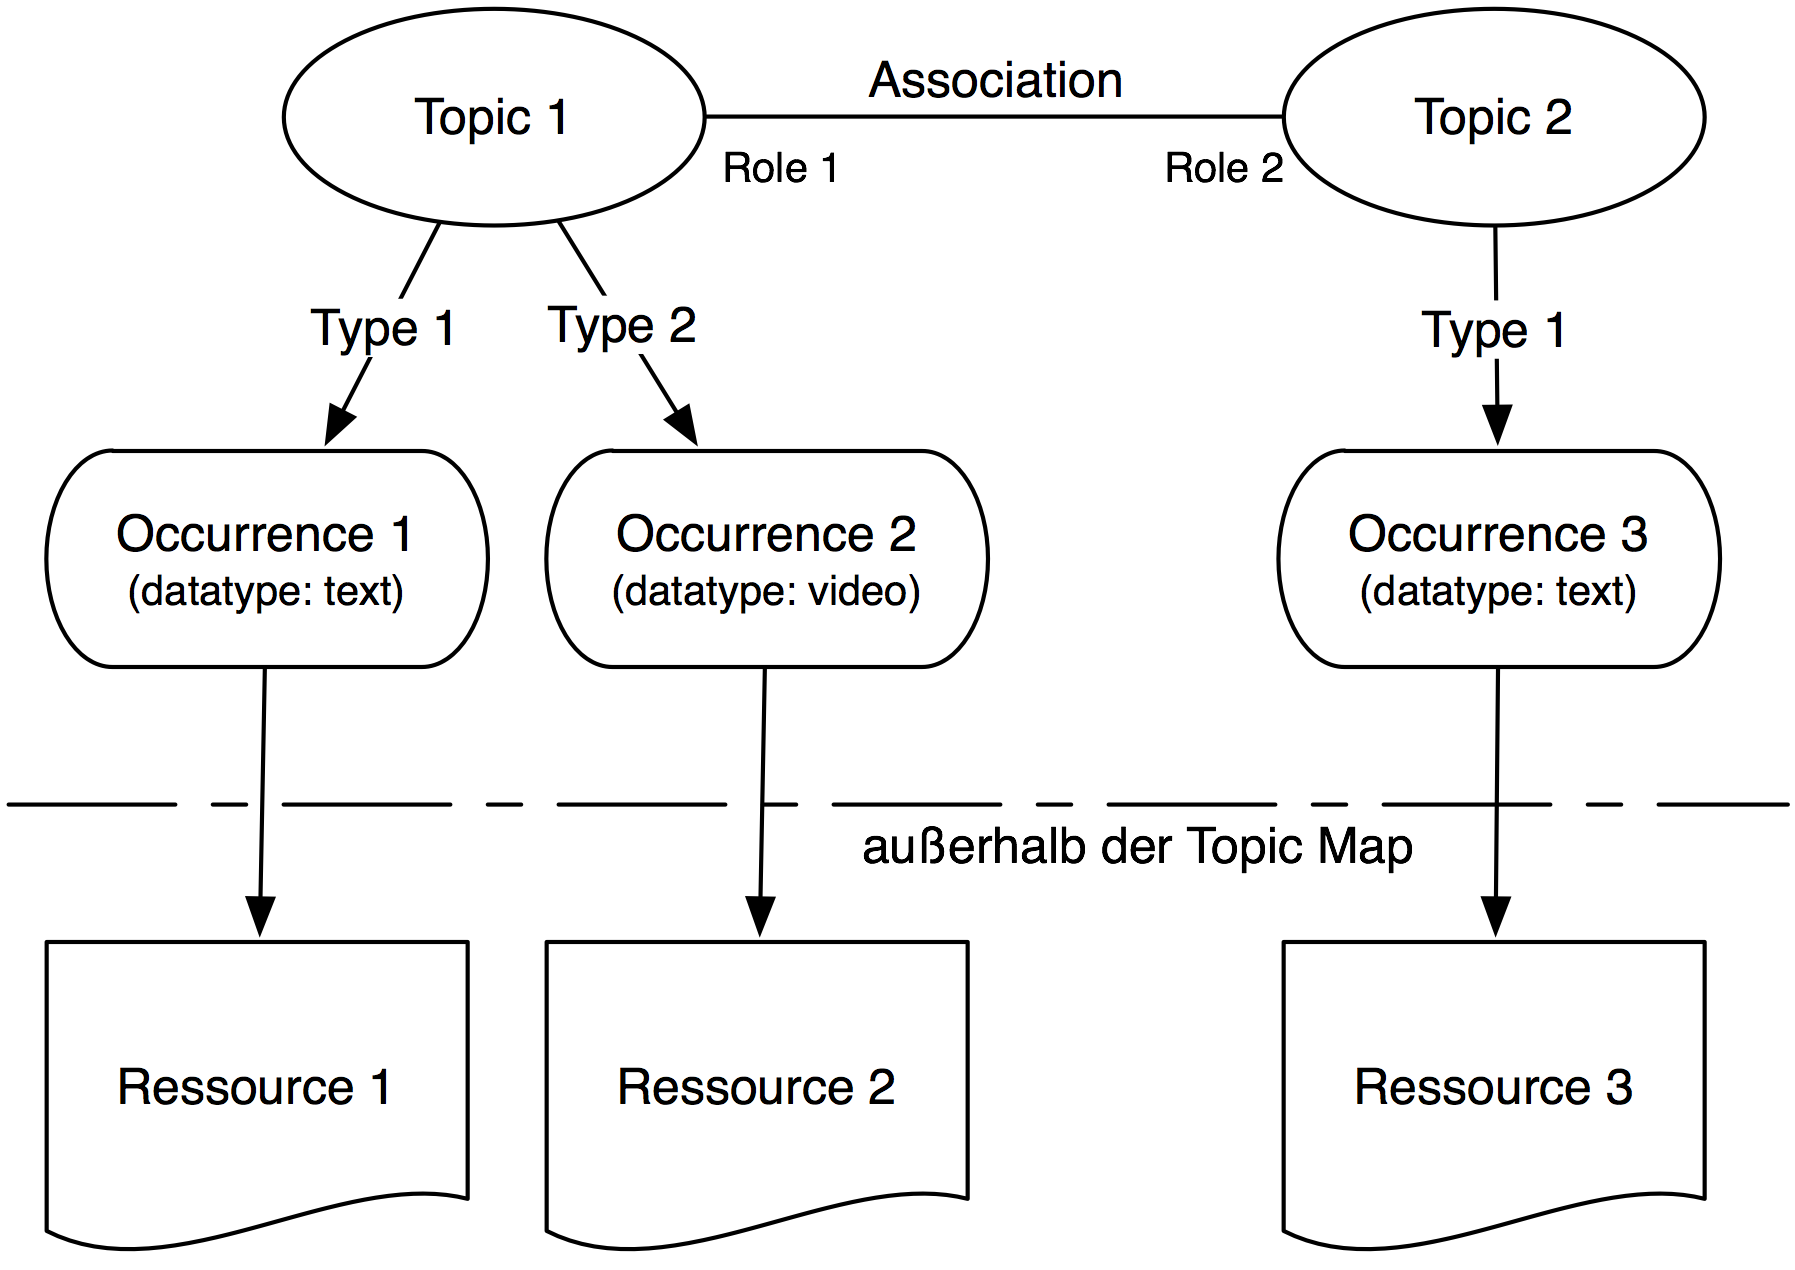
\includegraphics[width=10cm]{img/Persistenz/TMBasic.png}
	\caption{Grundlegende Elemente einer Topic Map}
	\label{fig:img_Persistenz_TMBasic}
\end{figure}

„Topics“ sind stellen Begriffe dar und bilden die Knoten des semantischen Netzes. Ein Topic kann beliebige Information darstellen, repräsentiert aber immer genau ein Phänomen der realen Welt (d.h. zu einem Topic muss es eine Entsprechung außerhalb der Topic Maps geben, die beobachtbar oder beschreibbar ist und auf die die modellierende Person Bezug nehmen will \footnote{„A subject can be anything whatsoever, regardless of whether it exists or has any other specific characteristics, about which anything whatsoever may be asserted by any means whatsoever. In particular, it is anything about which the creator of a topic map chooses to discourse.“ \citep[][S.8]{TMDM08}}). Eine Topic Map ist damit im Sinne von \citet{Stachowiak73} ein diagrammatisches Modell, das einen bestimmten, für den Modellersteller relevanten Ausschnitt der Realität abbildet.

“Associations“ bilden die Beziehungen zwischen Topics ab und stellen damit die Kanten des semantischen Netzes dar. Eine Association verknüpft Topics semantisch miteinander und kann frei mit Bedeutung belegt werden. Die Art der Beziehungen ist also nicht festgelegt und wird wie die Bedeutung der Topics frei gewählt werden. Topics und Associations decken historisch den Bereich der Darstellung von Thesauri ab, in denen Begriffe definiert und zueinanden in Beziehung gesetzt werden. 

Der zweite historische Ursprung von Topic Maps, die Indizes, werden durch das Konstrukt der „Occurences“ abgedeckt. Occurences (“Auftreten“) sind Referenzen aus der Topic Map in die reale Welt. Sie setzen die Topics einer Topic Map in Bezug zu beliebiger referenzierbarer Information (z.B. Dokumente). Im Kontext der eben genannten Indizes, kann eine Topic Map als der mit Querverweisen versehene Index eines Buches verstanden werden, in dem durch die Angabe von Seitenzahlen auf den Text des Buches verwiesen wird. Diese Verweise durch Angabe der Seitenzahlen sind in diesem Zusammenhang die Occurrences.

Die Ansammlung von durch Associations verknüpften und mit Occurrences versehenen Topics bilden eine Topic Map. Darüber hinaus kann in Topic Maps jedoch noch weiterführende Information repräsentiert werden (siehe Abbildung \ref{fig:img_Persistenz_TMFull}), die Gegenstand der folgenden Abschnitte sein werden.

\begin{figure}[htbp]
	\centering
		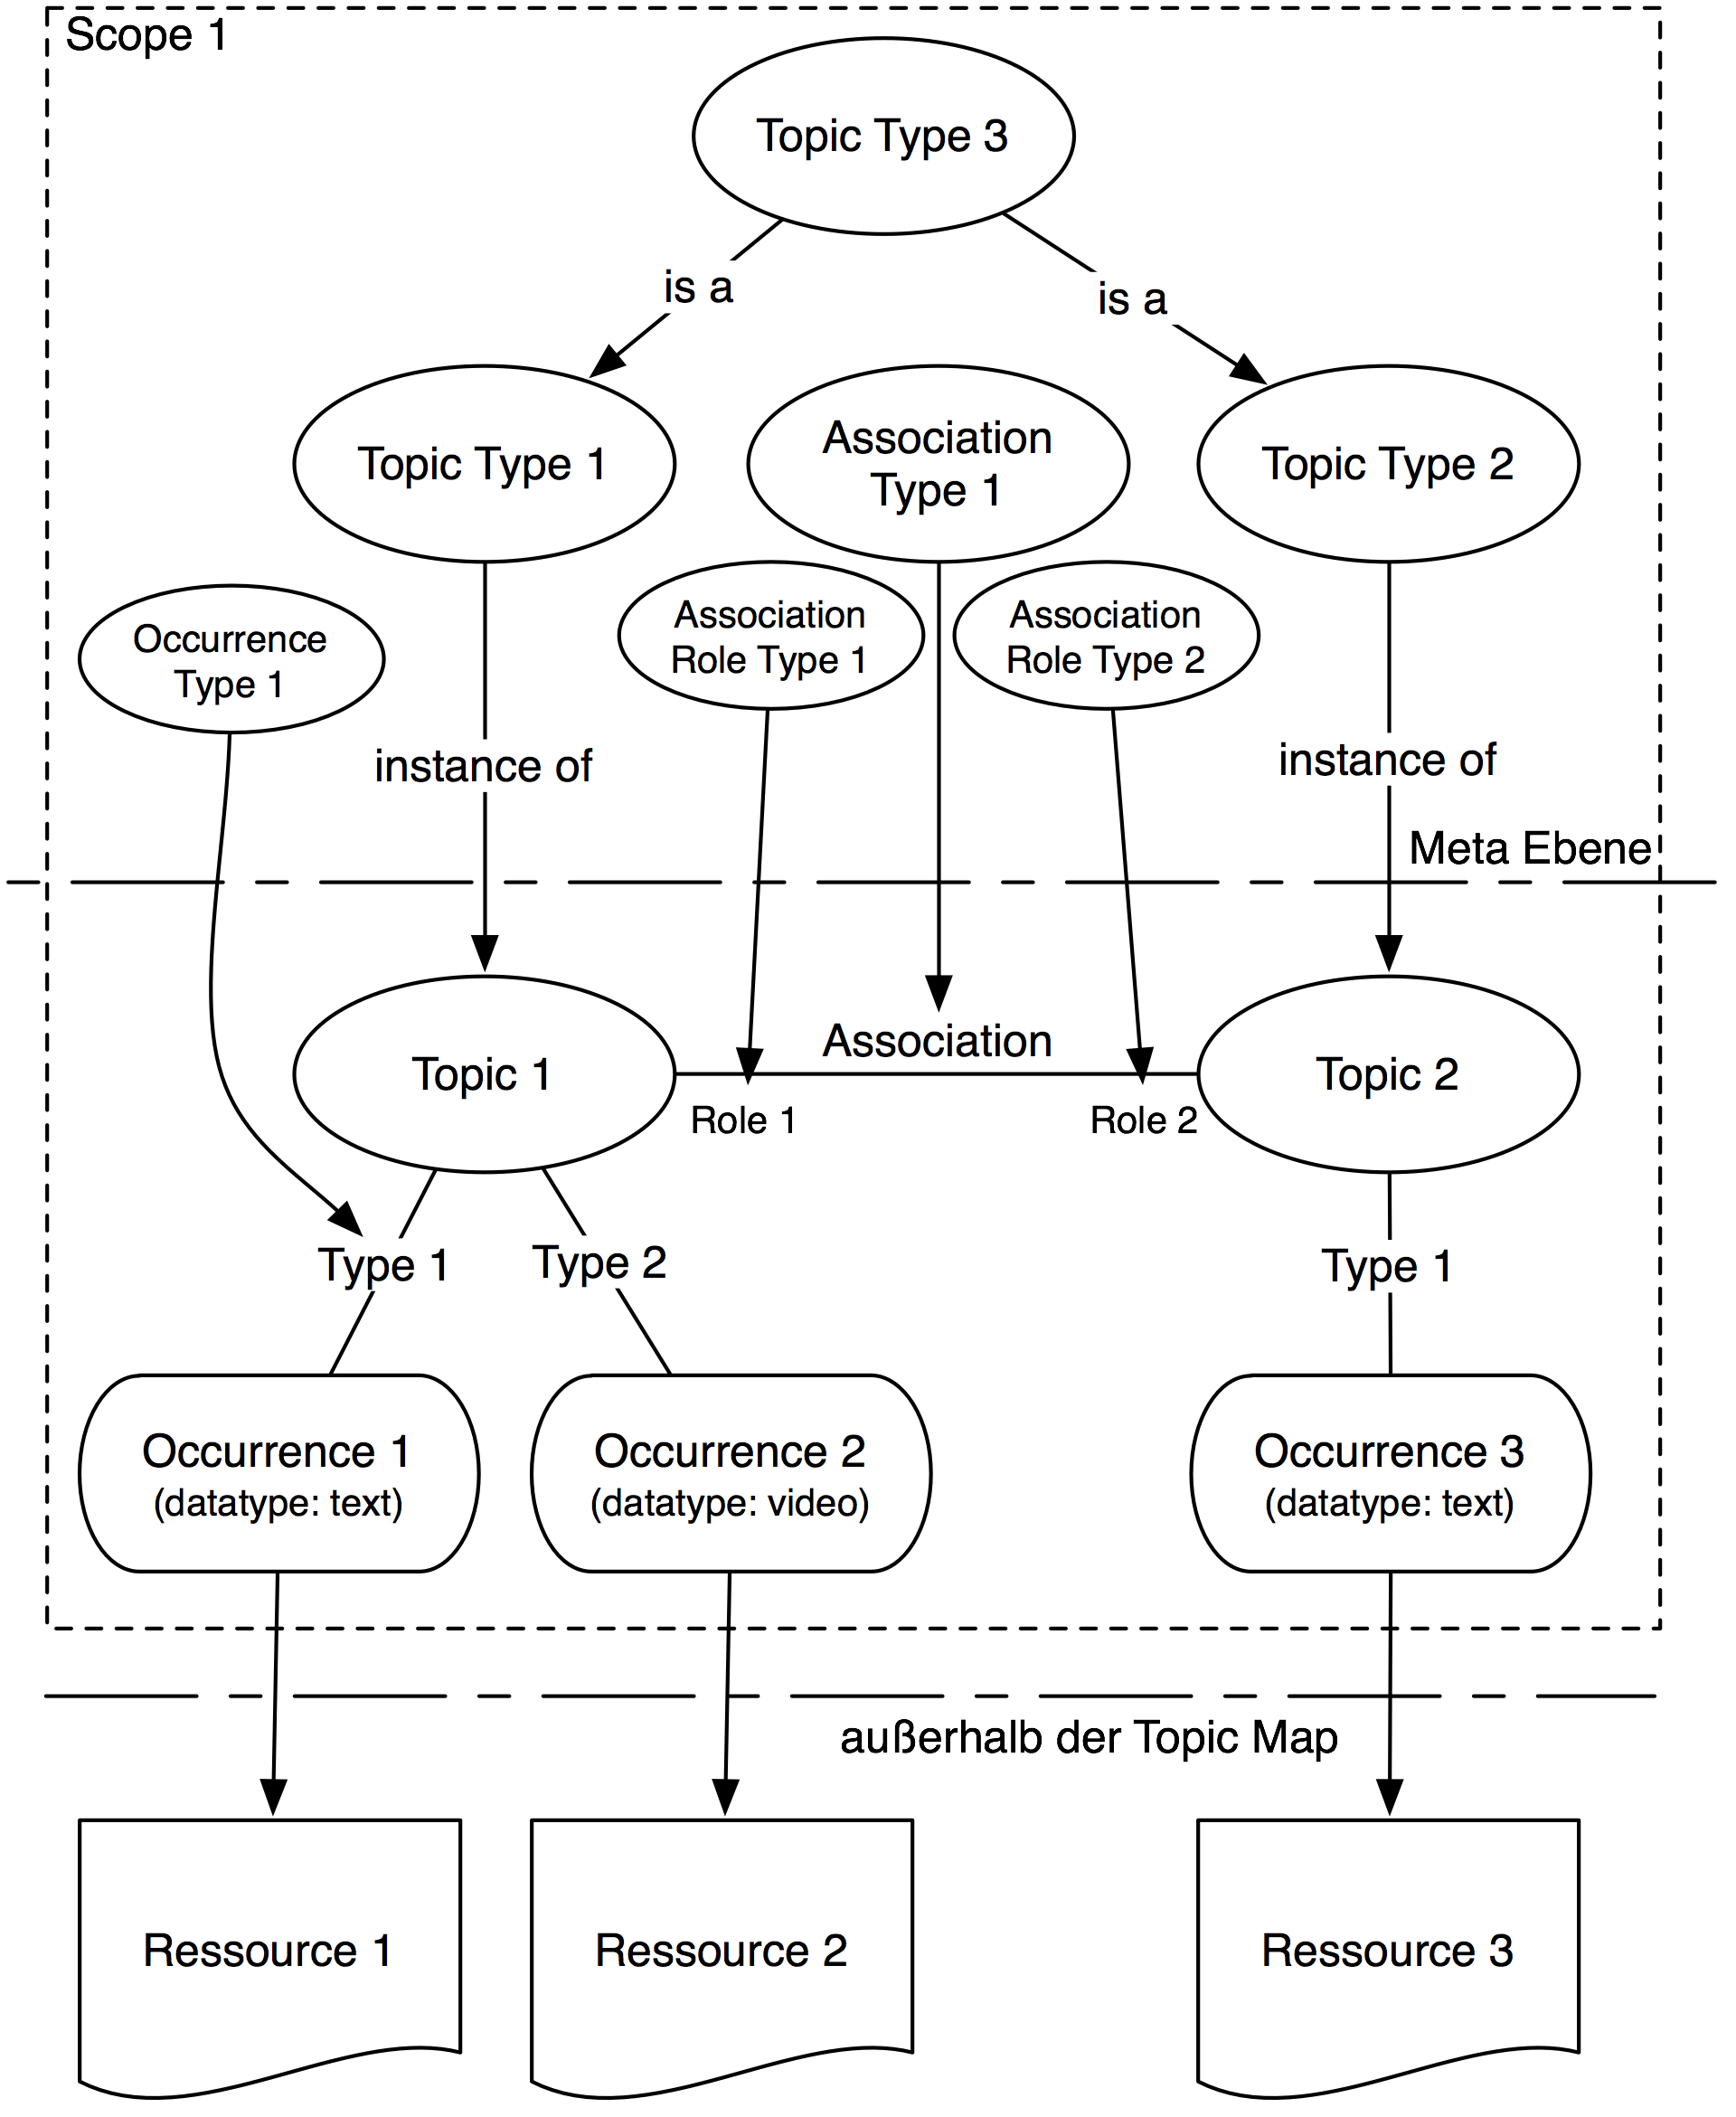
\includegraphics[width=10cm]{img/Persistenz/TMFull.png}
	\caption{Umfassende Darstellung der Elemente einer Topic Map}
	\label{fig:img_Persistenz_TMFull}
\end{figure}

\subsection{Topics, Subjects, Topic Names und Variants} % (fold)
\label{sub:topics_subjects_topic_names_und_variants}

Wie oben bereits beschrieben, repräsentiert ein Topic ein Phänomen der realen Welt in einer Topic Map. Dieses Phänomen der realen Welt, das durch das Topic repräsentiert wird, wird als „Subject“ bezeichnet. In einer Topic Map darf es zu einem Subject nur exakt ein Topic geben, umgekehrt kann ein Topic auch nicht mehrere Subjects repräsentieren, die Zuordnung zwischen Subject und Topic ist also eineindeutig (bijektiv). Im Topic wird dazu exakt ein „Subject Identifier“ registriert, der auf eine Informationsressource verweist, die das Subject für Menschen eindeutig identifizierbar macht (diese Ressource wird als „Subject Indicator“ bezeichnet). Zusätzlich kann ein „Subject Locator“ angegeben werden, der auf das tatsächlich in der realen Welt vorhandene Subject verweist. In Abgrenzung dazu kann es bei der anderen Brücke zwischen realer Welt und Topic Map, den Occurrences, für jeder Topic beliebig viele Zuordnungen geben. Eine Occurrence referenziert auch auf die reale Welt, zeigt aber dort nicht auf das Subject selbst, sondern auf ein dieses Subject beschreibendes Objekt in der realen Welt. Beispielhaft ist dazu in Abbildung \ref{fig:img_Persistenz_SubjectVsOccurrence} dieser Zusammenhang anhand des Topics „Tasse“ dargestellt. Ein anderes Beispiel ist ein Topic „London“, das als Subject die reale Stadt London repräsentiert und dem eine Occurrence zugeordnet werden könnte, die auf eine Landkarte (als in der Realität vorhandene Beschreibung der realen Stadt London) referenziert.

\begin{figure}[htbp]
	\centering
		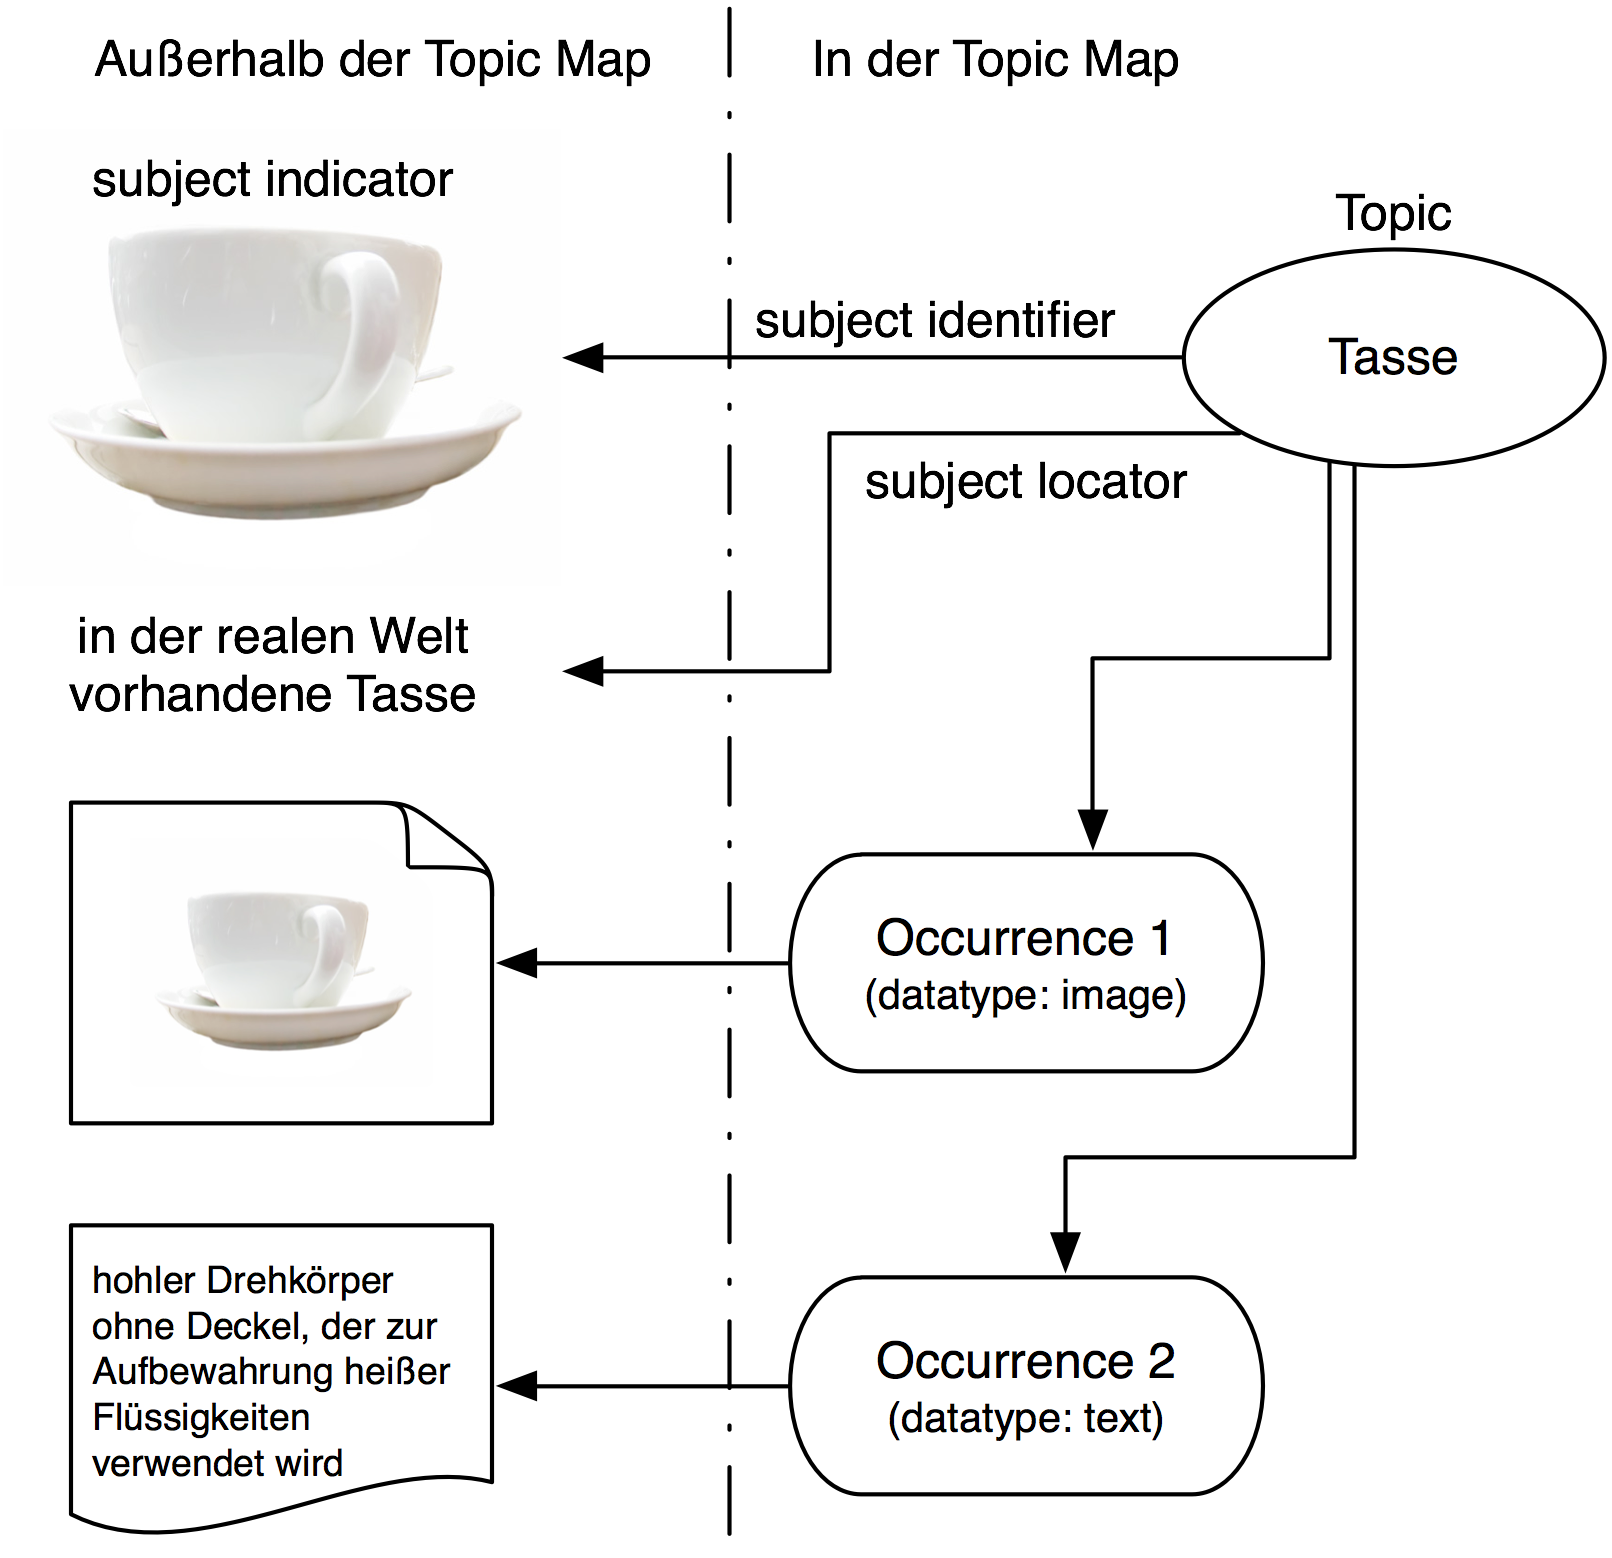
\includegraphics[width=10cm]{img/Persistenz/SubjectVsOccurrence.png}
	\caption{Abgrenzung zwischen Subject und Occurrence in Topic Maps}
	\label{fig:img_Persistenz_SubjectVsOccurrence}
\end{figure}

Bislang wurde vereinfacht ein Topic immer mit einem direkt zugeordneten Namen dargestellt. In einer Topic Map besitzt ein Topic jedoch keinen eindeutigen Namen. Es wird vielmehr durch seinen Subject Identifier eindeutig gekennzeichnet. Dieser ist jedoch nicht unbedingt für Menschen les- und/oder interpretierbar -- der Subject Identifier hat das Ziel, ein Subject für die Verarbeitung durch Software eindeutig zuordenbar zu machen. Für die Bezeichnung eines Topics in einer für Menschen interpretierbaren Form ist die Verwendung von „Topic Names“ vorgesehen (siehe Abbildung \ref{fig:img_Persistenz_TopicNaming}). Topic Names werden immer textuell angegeben und beschreiben das Subject, das durch das betreffende Topic referenziert wird. Durch einen Topic Name soll das Subject für Menschen erkennbar sein, wobei die Zuordnung nicht notwendigerweise eindeutig sein muss (Beispiel: der Topic Name „Jaguar“ kann ein Fahrzeug oder eine Großkatze bezeichnen und ist dementsprechend ein zulässiger Name für zwei unterschiedliche Topics). Einem Topic können beliebig viele Topic Names zugewiesen werden -- es ist so zum Beispiel möglich, eine mehrsprachige Topic Map zu realisieren, in der zu jedem Topic Topic Names in unterschiedlichen Sprachen angegeben werden. 

\begin{figure}[htbp]
	\centering
		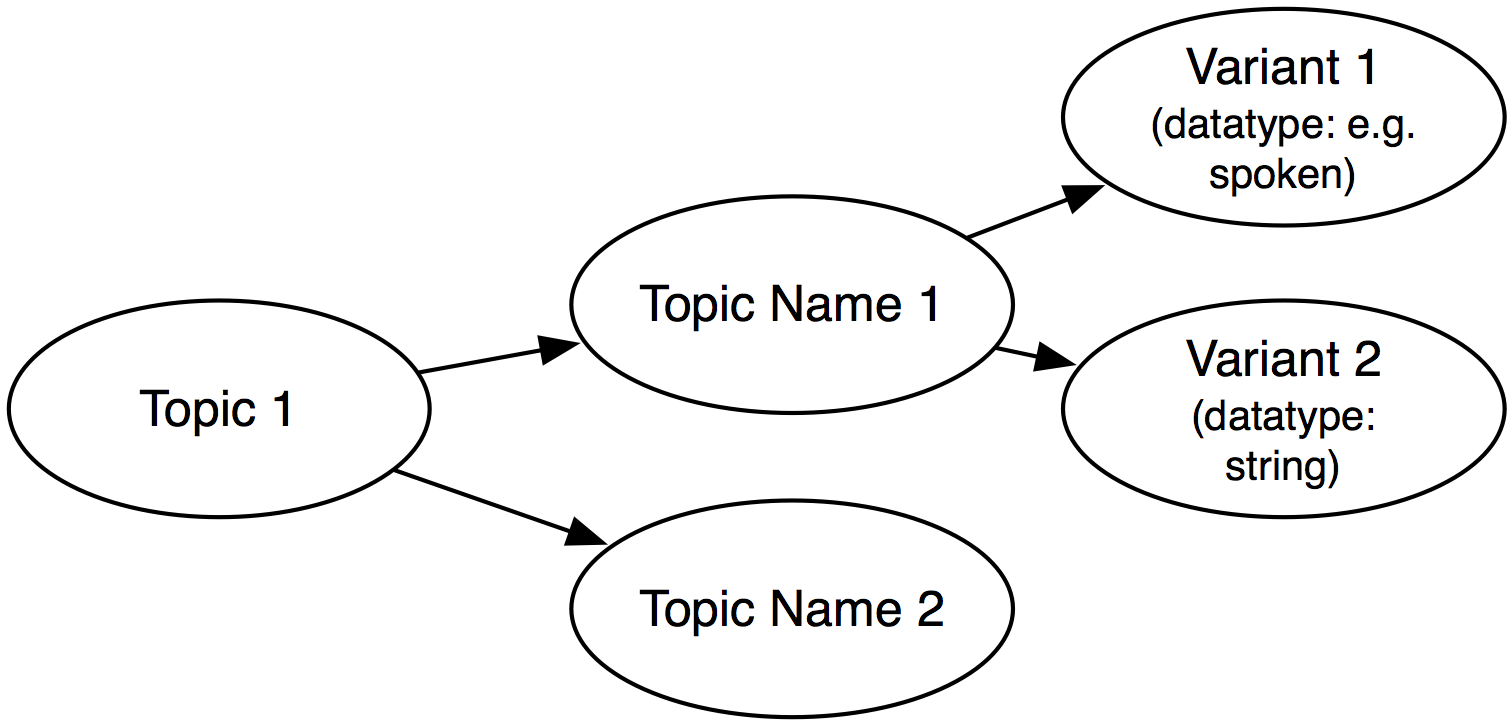
\includegraphics[width=10cm]{img/Persistenz/TopicNaming.png}
	\caption{Benennung von Topics}
	\label{fig:img_Persistenz_TopicNaming}
\end{figure}

Als weitere Detaillierungsstufe können zu jedem Topic Name „Variants“ angegeben werden. Wie durch den Namen angedeutet, handelt es sich dabei um Varianten eines Topic Names, die in bestimmten Zusammenhängen oder für gewisse Anwendungszwecke besser geeignet sein können als der eigentlich Topic Name. Ein Beispiel für eine mögliche Variante ist die Angabe einer gesprochenen Version des Topic Names. Ein weiteres Anwendungsgebiet für Varianten ist die im Standard explizit vorgesehene Angabe eines „Sort Name“ \citep[][S. 18]{TMDM08}, der es erlauben soll, Topic Maps in eine durch diesen Namen vorgegebene Ordnung bringen zu können. Varianten werden durch die Angabe eines dezidiert dafür gewidmeten Topics in deren Scope (siehe Abschnitt \ref{sub:scopes}) als Sort Names gekennzeichnet.

% subsection topics_subjects_topic_names_und_variants (end)

\subsection{Associations und Roles} % (fold)
\label{sub:associations_und_roles}

“Associations“ stellen Verbindungen zwischen den einzelnen Topics einer Topic Map her. Associations haben beliebig viele Endpunkte, mindestens jedoch einen (sind also nicht von vorneherein immer binär sondern können auch unär sein oder mehr als zwei Topics verknüpfen). Eine Associations enthält wie ein Topic nicht unmittelbar einen für Menschen lesbaren Namen. Diese wird durch ein Topic festgelegt, das die Kategorie festlegt, der die Association zuzuordnen sind (siehe Abschnitt \ref{sub:metamodellierung_in_topic_maps}). Diesem Topic kann wiederum mindestens ein Topic Name zugeordnet werden, welcher letzendlich die Benennung der Association festlegt.

Associations werden jedoch nicht direkt mit Topics verknüpft. Um ausdrucksstärkere Verknüpfungen realisieren zu können, agieren „Roles“ als Verknüpfung zwischen Association und den betreffenden Topics. Roles legen die „Rolle“ -- also die Bedeutung -- eines Topics in exakt der betrachteten Association fest. Diese Bedeutung kann generisch sein und zum Beispiel dazu verwendet werden, die per se ungerichteten Associations unabhängig von ihrer konkreten Bedeutung mit einer Richtung zu versehen (zum Beispiel durch die Zuordnung von Roles „Anfang“ und „Ende“) aber auch um die Beziehung semantisch anzureichern (zum Beispiel durch die Zuordnung von Roles „Veranwortlicher“, „Ausführender“ und „Prozessschritt“ in einer Association „durchzuführen“). Die Anzahl der in einer Association referenzierten Roles gibt damit auch die Kardinalität der Association (also die Anzahl ihrer Endpunkte) an. Aus den konkreten Roles wird dann auf die Topics verwiesen, die diese Roles einnehmen bzw. „spielen“ (tatsächlich heißt die betreffende Eigenschaft einer Role „player“). Genau wie Associations werden Roles nicht direkt benannts sondern über ein Topic, das ihre Kategorie bestimmt, mit einer Benennung versehen (Detail wiederum in Abschnitt \ref{sub:metamodellierung_in_topic_maps}).

% subsection associations_und_roles (end)

\subsection{Occurrences und Datatypes} % (fold)
\label{sub:occurrences_und_datatypes}

Wie zu Beginn dieses Abschnitts bereits beschrieben und in den Erläuterungen zur Thematik der Subjects (siehe Abschnitt \ref{sub:topics_subjects_topic_names_und_variants}) angedeutet, bilden „Occurrences“ die Brücke aus der Topic Map in die reale Welt, indem sie auf Ressourcen referenzieren, die in einem beliebigen Zusammenhang mit den jeweiligen Topic stehen. Ein Topic kann beliebig viele Occurrences haben. Anders als bei Associations existieren für Occurrences keine Roles (was auch nur bedingt sinnvoll wäre, da jede Occurrence nur zu exakt einem Topic gehören kann). Die Bedeutung der Occurrence für das Topic kann wie bei Associations über die Kategorie der Occurrence festgelegt werden, die wiederum durch ein separates Topic repräsentiert wird (siehe dazu auch Abschnitt \ref{sub:metamodellierung_in_topic_maps}). Beispielsweise kann eine Occurrence zur Kategorie „Karte“ gehören und so angeben, dass die so klassifizierte Occurrence zum Topic „London“ auf eine Karte des Stadtgebiets verweist.

Zusätzlich zu der Kategorie wird in einer Occurrence auch der Datentyp der Information angegeben, in dem die referenzierte Information vorliegt. Dabei können beliebige URI (Uniform Resource Identifiers\footnote{wie in RFC 3986 definiert und unter http://www.ietf.org/rfc/rfc3986.txt abzurufen}) verwendet werden. Da URIs beliebigen Inhalt haben können, wäre es in obigen Beispiel möglich durch den Datentyp einer Occurrence festzulegen, ob es sich bei der Karte um eine Rastergrafik oder eine Vektorgrafik handelt und so Information über deren möglich Einsatzgebiete zu einzubetten.

% subsection occurrences_und_datatypes (end)

\subsection{Metamodellierung in Topic Maps} % (fold)
\label{sub:metamodellierung_in_topic_maps}

Wie oben bereits mehrmals angedeutet kann in einer Topic Map neben den eigentlichen zu repräsentierenden Informationen (Topics, Associations, Roles und Occurrences) auch Information über die Topic Map selbst eingebettet werden (neben dem Model also auch das Meta-Modell abgebildet werden kann). Die Information umfasst Angaben über die in der jeweiligen Topic Map existierenen Kategorien von Topics, Topic Names, Associations, Roles und Occurrences. Hinsichlich der Repräsentation dieser Information sind zwei Ansätze zu unterscheiden, von denen der erste bei Kategorieangaben von Topics zum Einsatz kommt, der andere bei Kategorieangaben jeder anderen Art von Information. Allen Kategorien ist gemein, dass sie selbst wiederum als Topics repräsentiert werden und auch als solche verwendet werden können. Es ist also möglich, zu einem Topic, das als Kategorie verwendet wird, selbst wiederum eine Kategorie anzugeben, wodurch die Einführung beliebig vieler Meta-Ebenen möglich ist. Außerdem können als Kategorien verwendete Topics ebenfalls wieder mit Associations verknüpft und mit Occurrences versehen werden. Hinsichtlich der Nomenklatur ist noch darauf hinzuweisen, dass Kategorien im Allgemeinen als „Types“ bezeichnet werden, man also von „Topic Types“, „Topic Name Types“, „Association Types“, „Role Types“ und „Occurrence Types“ spricht.

\subsubsection{Topic Types}

Topic Types werden in einer Topic Map durch ein spezielle, im Standard festgelegte Association definiert. Soll einem Topic ein Type zugewiesen werden, muss eine Association der Kategorie „type-instance“ eingefügt werden, bei der das Topic selbst die Role „instance“ einnimmt und dem Topic, das die Kategorie repräsentiert, die Role „type“ zugewiesen wird. Diese Beziehung entspricht einer Konkretisierung eine (abstakten) Kategorie oder Klasse von Topics auf eine bestimmte Instanz, die die Merkmale dieser Klasse trägt. In Abbildung \ref{fig:img_Persistenz_MetaModelExample} besteht eine type-instance-Beziehung (dort als „instance-of“ bezeichnet) zwischen der Kategorie „VW Golf“ und der konkreten Instanz „SR-174 AU“ (also einem Topic, bei dem das amtliche Kennzeichen als Topic Name verwendet wurde). „VW Golf“ fungiert hier also als Topic Type, wobei es selbst ein Topic ist, das sich durch nichts als die eingenomme „type“-Rolle von einem anderen Topic unterscheidet und dementsprechend behandelt werden kann.

Einem Topic können beliebig viele Topic Types zugewiesen werden, indem es in mehr als einer Association die Role „instance“ einnimmt. Es wird so als mehreren Kategorien zugehörig gekennzeichnet. Umgekehrt kann ein Topic Type mehr als einem Topic zugewiesen werden, indem das betreffende den Topic Type repräsentierende Topic die Role „type“ mehrfach einnimmt.

\begin{figure}[htbp]
	\centering
		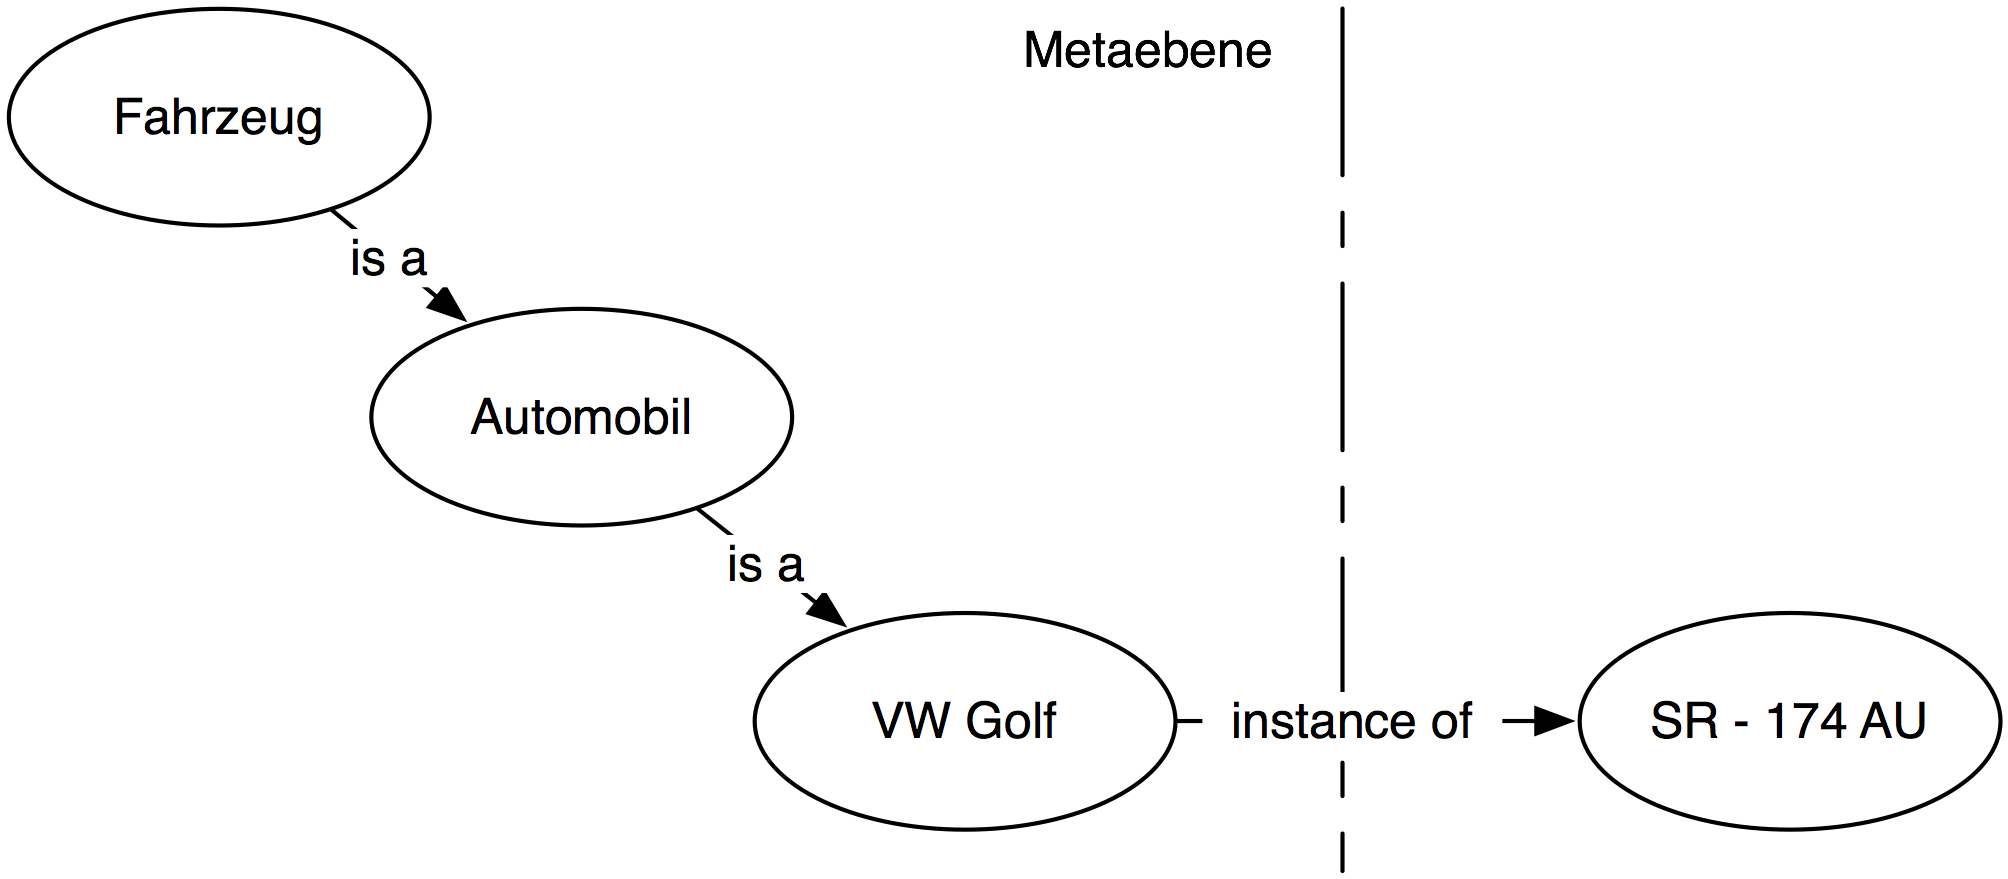
\includegraphics[width=10cm]{img/Persistenz/MetaModelExample.png}
	\caption{Beziehungen in der Metamodellbildung in Topic Maps}
	\label{fig:img_Persistenz_MetaModelExample}
\end{figure}

Auch ist es möglich, Hierarchien von Types zu bilden, in dem einem Topic, das als Topic Type fungiert, selbst wieder ein Topic Type zugewiesen wird. Dieses Konstrukt ist jedoch mit Vorsicht zu gebrauchen, da zur Abbildung der Struktur einer Domäne ein semantisch ähnliches, bei näherer Betrachtung aber eine unterschiedliche Bedeutung tragendes Konstrukt zum Einsatz kommt. Grundsätzlich muss unterschieden werden, ob ein Topic eine konkrete Instanz eines anderen ist oder lediglich eine Spezialisierung darstellt. Im ersteren Fall kommt eine „type-instance“ zum Einsatz, das übergeordnete Topic befindet sich semantisch auf eine anderen, abstrakteren Ebene und stellt eine Kategorie (also einen Topic Type) dar. Im Falle einer Spezialisierung kommt eine „supertype-subtype“-Association zum Einsatz, deren Rollen „supertype“ vom übergeordneten, allgemeineren bzw. „subtype“ vom untergeordneten, spezielleren Topic eingenommen wird. Hier befinden sich beide Topics semantisch auf einer Ebene, keines ist abstrakter als das andere. Der Unterschied liegt vielmehr in der mehr oder weniger konkreten Festlegung der durch die Topics repräsentierten Subjects. So ist wie in Abbildung \ref{fig:img_Persistenz_MetaModelExample} dargestellt das Topic „VW Golf“ ein Subtype des Topics „Automobil“ welches wiederum ein Subtype des Topics „Fahrzeug“ ist. Hier ist erkennbar, dass „Automobil“ insofern eine Spezialisierung von „Fahrzeug“ ist, als dass es im Allgemeinen motorisiert ist und vier Räder besitzt. „VW Golf“ ist wiederum eine Spezialisierung von Fahrzeug, die hinsichtlich der Form der Karosserie, der Anzahl der Türen und anderen Merkmalen mehr spezialisiert. Zwischen keinem der Topics findet jedoch eine Konkretisierung in dem Sinne statt, als dass auf der untergeordneten Seite von einem konkreten, real existierenden Fahrzeug die Rede wäre -- dazu ist die „type-instance“-Beziehung zu verwenden. Die „subtype-supertype“-Beziehung ist transitiv, d.h. dass ein „VW Golf“ nicht nur ein „Automobil“ ist, sondern auch ein „Fahrzeug“. Für „type-instance“-Beziehungen ist diese Eigenschaft nicht gegeben. 

\subsubsection{Andere Types}

Bei allen anderen Types (konkret also Topic Name Types, Association Types, Role Types und Occurrence Types) wird die Kategorie nicht durch eine separate Association abgebildet sondern durch eine im jeweiligen Informationselement enthaltene Referenz auf ein Topic, das als Type fungiert. Die Darstellung der Kategorie-Information ist damit nicht so explizit wie bei Topic Types, wo sich direkt in der Repräsentation der eigentlichen Nutzinformation niederschlägt. Auch semantisch ist sind die hier behandelten Types gegenüber Topic Types insofern eingeschränkt, als das jedem Element exakt ein Type zugeordnet sein muss (der Type kann also nicht leer sein, auch können nicht mehrere Types zugeordnet werden). Wie oben bereits erwähnt sind Topic Types hier flexibler, einem Topic können beliebig viele oder auch keine Topic Types zugeordnet werden. Dies ist aber nur vordergründig eine Einschränkung. Topics dürfen wie oben beschrieben für jedes Subjekt nur einmal existieren. Hat aber ein Subject und damit ein Topic in unterschiedlichen Domänen unterschiedliche Bedeutungen, muss dies über mehrere Topic Types (in Verbindung mit Scopes, siehe Abschnitt \ref{sub:scopes}) abgebildet werden. Alle anderen Informationskategorien in der Topic Map unterliegen nicht dieser Eineindeutigkeitsregel und können bzw. müssen, sollten sie unterschiedlichen Kategorien zuzuordnen sein, auch mehrfach vorhanden sein. Eine Assoziation, die einen anderen Namen trägt (also einer anderen Kategorie angehört) ist beispielsweise nicht identisch mit der ursprünglichen Assoziation, deren Name ebenfalls bereits durch die Zuordnung zu einer Kategorie festgelegt wurde. 

\subsubsection{Modellieren von Einschränkungen}

Der Topic Map Standard erlaubt zwar die Angabe von Metamodellelementen (Types), ermöglicht es aber nicht Regeln anzugeben, anhand derer der semantisch korrekte Aufbau einer Topic Map geprüft werden. Ed ist beispielsweise möglich, einen Association-Type „hat Mitglieder“ zu definieren, der mittels den Roles „Organisationseinheit“ und „Mitarbeiter“ die Zuordnung von Mitarbeitern zu den Organisationseinheiten eines Unternehmens zuzuordnen. Es ist jedoch in der Topic Map nicht möglich zu spezifizieren, das beispielsweise mindestens drei Mitarbeiter zugeordnet werden müssen oder das es in dieser Beziehung nur eine Organisationseinheit geben darf. Weiters kann nicht spezifiziert werden, durch Topics welchen Types die jeweiligen Roles eingenommen werden dürfen -- beispielsweise ist eine Zuordnung von Produktionsmitteln in der Role „Mitarbeiter“ zulässig bzw. kann sie nicht als unzulässig gekennzeichnet werden.

Ist eine derartige semantische Einschränkung bei der Topic Map Erstellung und die Einführung verbindlicher Strukturvorgaben notwendig, so muss dies außerhalb der Topic Map oder durch externe Interpretation spezifischer Topic Map Elemente geschehen. In ersterem Fall kann die noch finalem Zustand vorliegende TMCL (Topic Map Constraint Language, \citep{TMCL08}), eine Regelsprache zur Einschränkung der Repräsentationsmöglichkeiten in einer Topic Map, verwendet werden. Im zweiten Fall können die Metamodell-Elemente (also alle Topics, die als Types verwendet werden) durch zusätzliche Associations verknüpft werden, die semantisch so interpretiert werden, dass sie eine zulässige Kombination von Topics der jeweiligen Kategorie anzeigen.

% subsection metamodellierung_in_topic_maps (end)

\subsection{Statements und Scopes} % (fold)
\label{sub:scopes}

Topic Maps bieten die Möglichkeit, Gültigkeitsbereiche für die in ihnen abgebildeten Informationen zu spezifizieren. Ein Gültigkeitsbereich definiert, in welchem Kontext eine Information gültig ist. Außerhalb dieses Kontext kann über die Gültigkeit keine Aussage getroffen werden. Der Gültigkeitsbereich wird als „Scope“ bezeichnet. Ein Scope kann für jedes „Statement“ in der Topic Map gesetzt werden. Statements sind alle „Aussagen“ über Topics, die in der Topic Map abgebildet werden, nicht aber Topics selbst. Als Statement werden Topic Names, Associations und Occurrences betrachtet. Roles und Variants besitzen keinen Scope, da sie keine direkte Aussage über Topics treffen, sondern nur im Zusammenhang mit Associations bzw. Topic Names existieren, deren Scope sich quasi auf sie vererbt.

Ein Scope für ein Statement wird durch die Angabe eines oder mehrerer Topics festgelegt. Wird kein Topic angegeben, so gilt der „unconstrainted scope“, das Statement ist unbeschränkt gültig. Topics zur Abbildung von Scopes können explizit angelegt werden (z.B. Topics „Deutsch“ und „Englisch“, die Sprach-Scopes ermöglichen, Topics „Tierwelt“ und „Transportwesen“ zur Domänenabgrenzung -- siehe Abbildung \ref{fig:img_Persistenz_Scope}), es ist jedoch grundsätzlich auch möglich, die Gesamtheit der Topics einer Domäne zur Definition eines betreffenden Scopes heranzuziehen (also alle in der Topic Map vorhandenen Topics, die Tiere repräsentieren, als Scope zu verwenden, um den Gültigkeitsbereich „Tierwelt“ abzubilden). Obwohl der Topic Map Standard hier explizit offen bleibt, erscheint jedoch erstere Variante hinsichtlich der Verwaltbarkeit aber auch der semantischen Vollständigkeit wegen als ratsamer (das Konzept „Tierwelt“ käme ansonsten z.B. nicht notwendigerweise vor, sondern wäre nur implizit vorhanden, was eine Auswertung schwierig macht).

\begin{figure}[htbp]
	\centering
		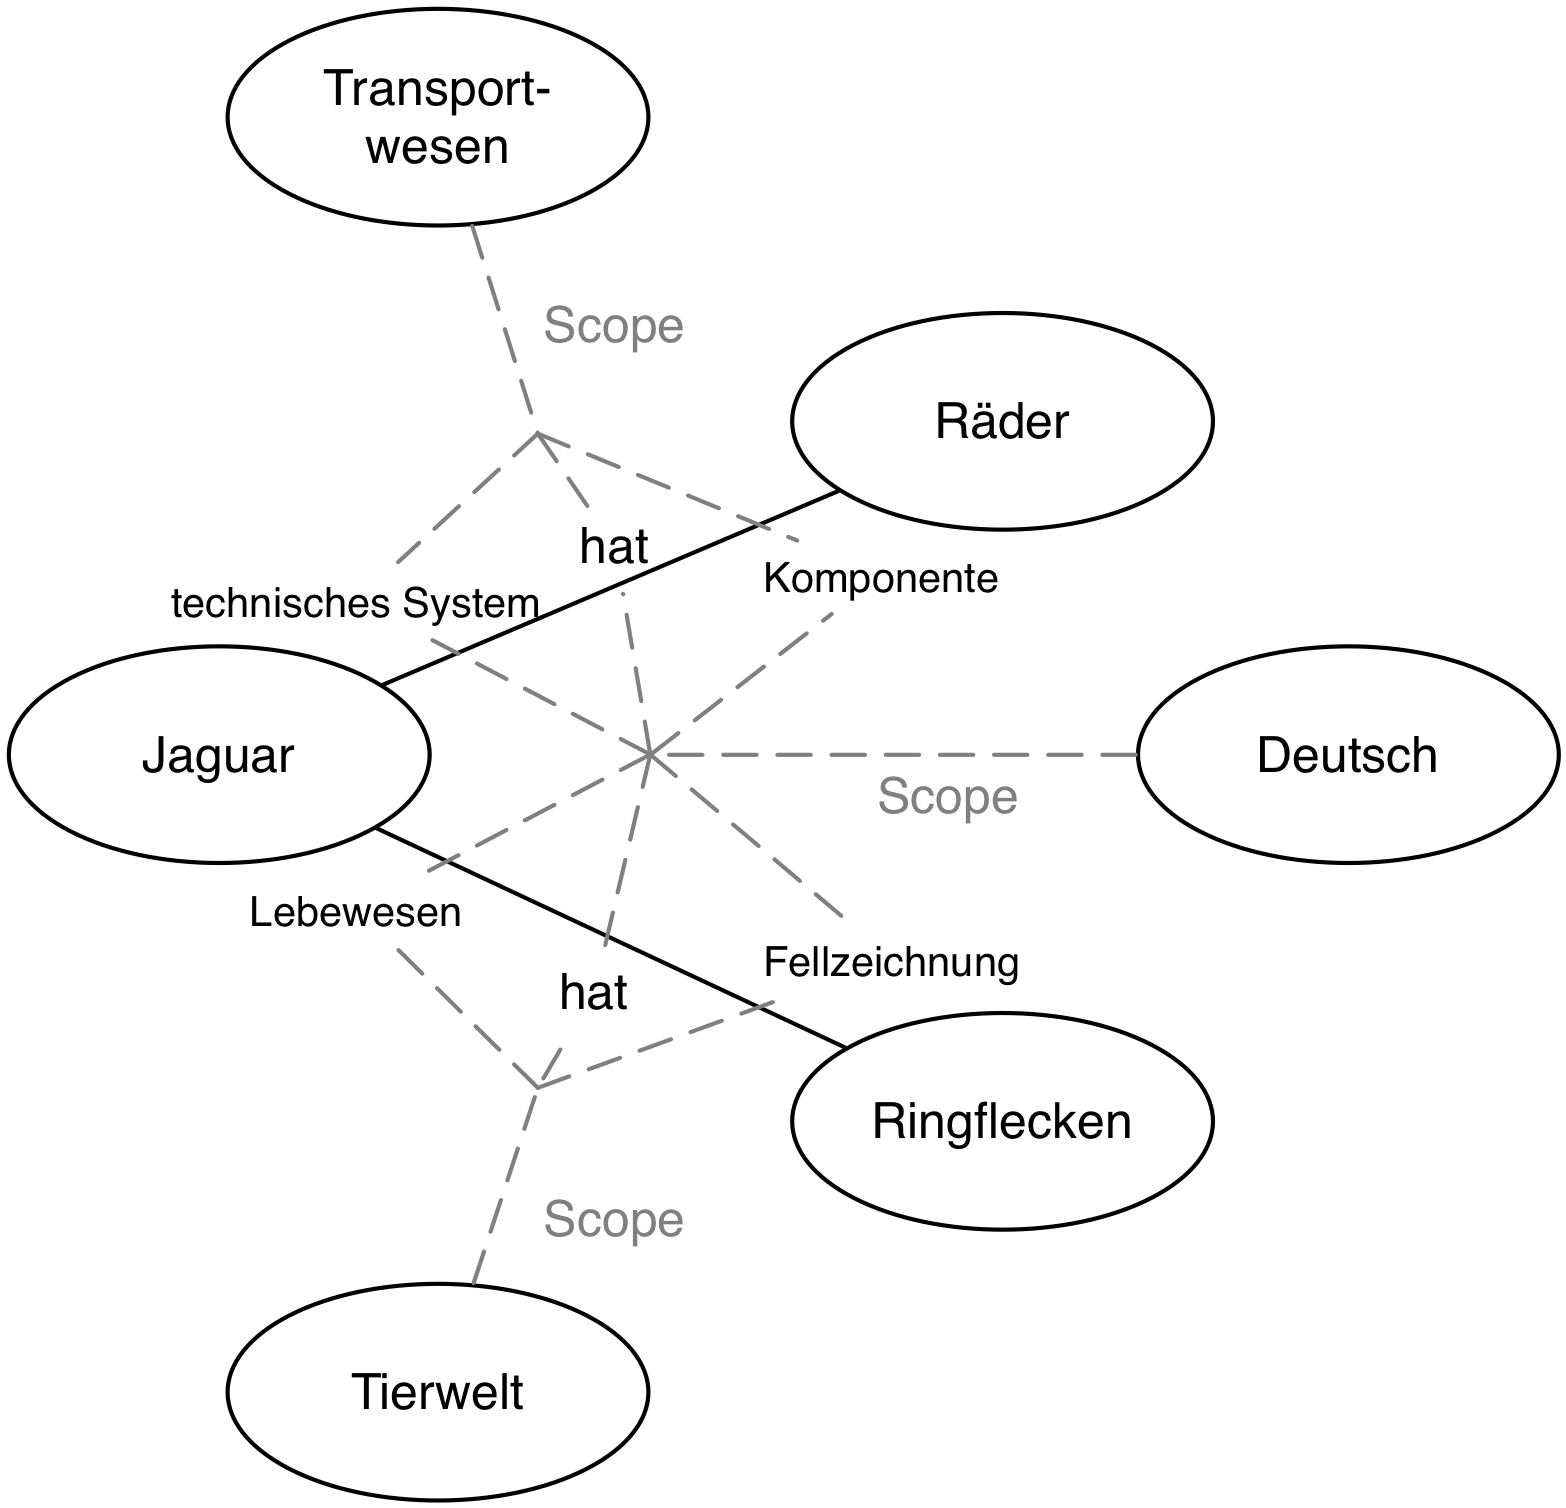
\includegraphics[height=3in]{img/Persistenz/Scope.png}
	\caption{Abbildung von Gültigkeitsbereichen durch Scopes}
	\label{fig:img_Persistenz_Scope}
\end{figure}


Wird mehr als ein Topic angegeben, so bilden alle Topics gemeinsam den Kontext, indem das Statement gültig ist. Bei der Auswertung des Gültigkeitsbereichs müssen also alle angegebenen Topics zutreffen, damit ein Statement gültig ist. Ein Statement dessen Scope die Topics „Tierwelt“ und „Deutsch“ enthält, ist also nur gültig, wenn beide Topics zutreffen (also z.B. zur Filterung ausgewählt wurden). Die gültigen Statements sind also die Schnittmenge jener der Statements, die im Scope „Tierwelt“ und im Scope „Deutsch“ gültig sind (siehe Abbildung \ref{fig:img_Persistenz_Scope}). Die Angabe eines Scopes zu einem Statement, das in beiden Scopes (unabhängig voneinander gesehen) gültig sein soll, ist nicht direkt möglich. In diesem Fall muss das Statement zweimal jeweils unter Angabe eines der beiden Scopes eingefügt werden.

Für Topics selbst kann kein Scope angegeben werden. Das ist hinsichtlich des Topic Maps zugrunde liegenden Konzepts auch nicht sinnvoll, da Topics immer ein Phänomen der realen Welt, das Subject, repräsentieren, das selbst immer vorhanden ist und dessen Gültigkeit bzw. Existenz nicht von anderen Rahmenbedingungen wie anderen Subjects abhängt. Dementsprechend existiert ein Topic immer, lediglich seine Bezeichnung, die Beziehungen zu anderen Topics oder seine Occurrences können abhängig vom einem Scope unterschiedlich sein.
% subsection scopes (end)

\subsection{Reification} % (fold)
\label{sub:reification}

Wie bereits zu Beginn angeführt, können in einer Topic Map beliebige Inhalte abgebildet werden, jegliche Phänomene der realen Welt können durch Topics repräsentiert werden. Konsequenterweise können nun auch Elemente der Topic Map selbst oder sogar die Topic Map ansich durch ein Topic dargestellt werden. Eine derartige selbstbezügliche Abbildung wird als „Reification“ bezeichnet. Der Ausgangspunkt für eine Reification kann ein Statement sein oder eine Topic Map selbst. Topics können nicht verwendet werden, da ein sie repräsentierendes Topic semantisch äquivalent mit dem Ausgangspunkt wäre und damit zwei Topics vorhanden wären, die das gleiche Subject referenzieren. Nachdem die Abbildung zwischen Subject und Topic eineindeutig sein muss, ist ein derartiges Konstrukt nicht erlaubt.

In Abgrenzung zur Types (Association Types, Occurrence Types, \ldots) repräsentiert ein reifizierendes Topic nicht die Kategorie eines Elements sondern das konkrete Element selbst. Es ist so möglich, einem konkreten Element wie einer Association zusätzliche Information hinzuzufügen (etwa eine Occurrence) oder auch eine bestehende Topic Map als Ganzes zu kapseln und durch das sie reifizierende Topic Bezug zu nehmen. 

% subsubsection reification (end)

\subsection{Merging} % (fold)
\label{ssub:merging}

Unter „Merging“ versteht man die Vereinigung zweier voneinander getrennter Topic Maps zu einer gemeinsamen Map. Dabei ist vor allem die Eineindeutigkeitsregel zu beachten, für ein Subject darf also in der resultierenden Topic Map nur ein Topic existieren. Strukturell nicht kritisch, jedoch die Verwendbarkeit einschränkend sind mehrfach auftretende semantisch identische Statements. Soweit möglich, sollten auch diese Duplikate im Merging-Prozess entfernt werden.

Der Topic Map Standard definiert für jede Art von Element Regeln, anhand der festgestellt werden kann, ob zwei Elemente dieser Art identisch sind oder nicht. Ausgangspunkt sind immer die Topics, wobei beim Vergleich ausschließlich vom abgebildeten Subject ausgegangen werden muss. Sind die Subjects identisch, sind im Wesentlichen auch die beiden Topics identisch und können durch eine gemeinsames Topic ersetzt werden. Auf Basis der vereinigten Topic Menge werden nun die enthaltenen Statements verglichen. Damit Statements als identisch erkannt werden, müssen nicht nur ihr eigentlicher Inhalt sondern auch ihre Kategorie (Type), ihr Gültigkeitsbereich (Scope) und das/die ihnen zugeordnete(n) anderen Element(e) identisch sein. Eine Role ist also nur dann mit einer anderen Role identisch, wenn ihr Type, ihr Scope, die Association, der sie angehört und das referenzierte Topic identisch ist. Daraus folgt, das in der Merging-Reihenfolge zuerst die Topics, dann die eigenständigen Statements wie Topic Names, Associations und Occurrences und letztendlich die abgängigen Statements wie Roles und Variants behandelt werden müssen.
% subsubsection merging (end)

% section topic_maps (end)

\section{Abbildung von Modellen auf Topic Maps} % (fold)
\label{sec:abbildung_von_modellen_auf_topic_maps}

Diagrammatische Modelle \citep{Oppl05a} können direkt ohne zusätzliche Transformationen auf Topic Maps abgebildet werden. Derartige Modelle bestehen aus Knoten und Kanten, die Verwendung dieser im konkreten Anwendungskontext ist durch die Modellierungssprache festgelegt. In den folgenden Abschnitten wird nun beschrieben, wie die einzelnen Aspekte eines diagrammatischen Modells auf eine Topic Map abgebildet werden können.

\subsection{Grundlegende Abbildung} % (fold)
\label{sub:grundlegende_abbildung}
Der nahe liegendste Ansatz, um diagrammatische Modelle auf Topic Maps abzubilden, werden nun die Knoten auf Topics, die Kanten auf Associations abzubilden (siehe Abbildung \ref{fig:img_Persistenz_AssociationReification}, Variante 1). Ist in den Kanten mehr Information als die bloße Anzeige der Verbindung von zwei Knoten abgebildet (wie z.B. in \gls{UML} State Charts \citep{Rumbaugh04}, bei denen die zu einem Zustandsübergang führenden Ereignisse inkl. Bedingungen und ablaufende Aktionen in den Kanten repräsentiert werden), so kann es sinnvoll sein, auch die Kanten auf Topics abzubilden, da diesen auf dem Wege der Occurrences zusätzliche Information zugewiesen werden kann (siehe Abbildung \ref{fig:img_Persistenz_AssociationReification}, Variante 2). Associations würden in diesem Fall verwendet, um die Knoten und Kanten des Modells zu verbinden, spielen also in der Repräsentation der Information nur noch ein untergeordnete Rolle. Ein Weg, die direkte Abbildung beizubehalten (indem Knoten auf Topics und Kanten auf Associations abgebildet werden) ist, zur Repräsentation der zusätzlich in den Kanten liegenen Information die Möglichkeit der Reification zu nutzen, den Associations also Topics zuzuweisen, die genutzt werden können, um diese zusätzliche Information zu verwalten (siehe Abbildung \ref{fig:img_Persistenz_AssociationReification}, Variante 3).

\begin{figure}[htbp]
	\centering
		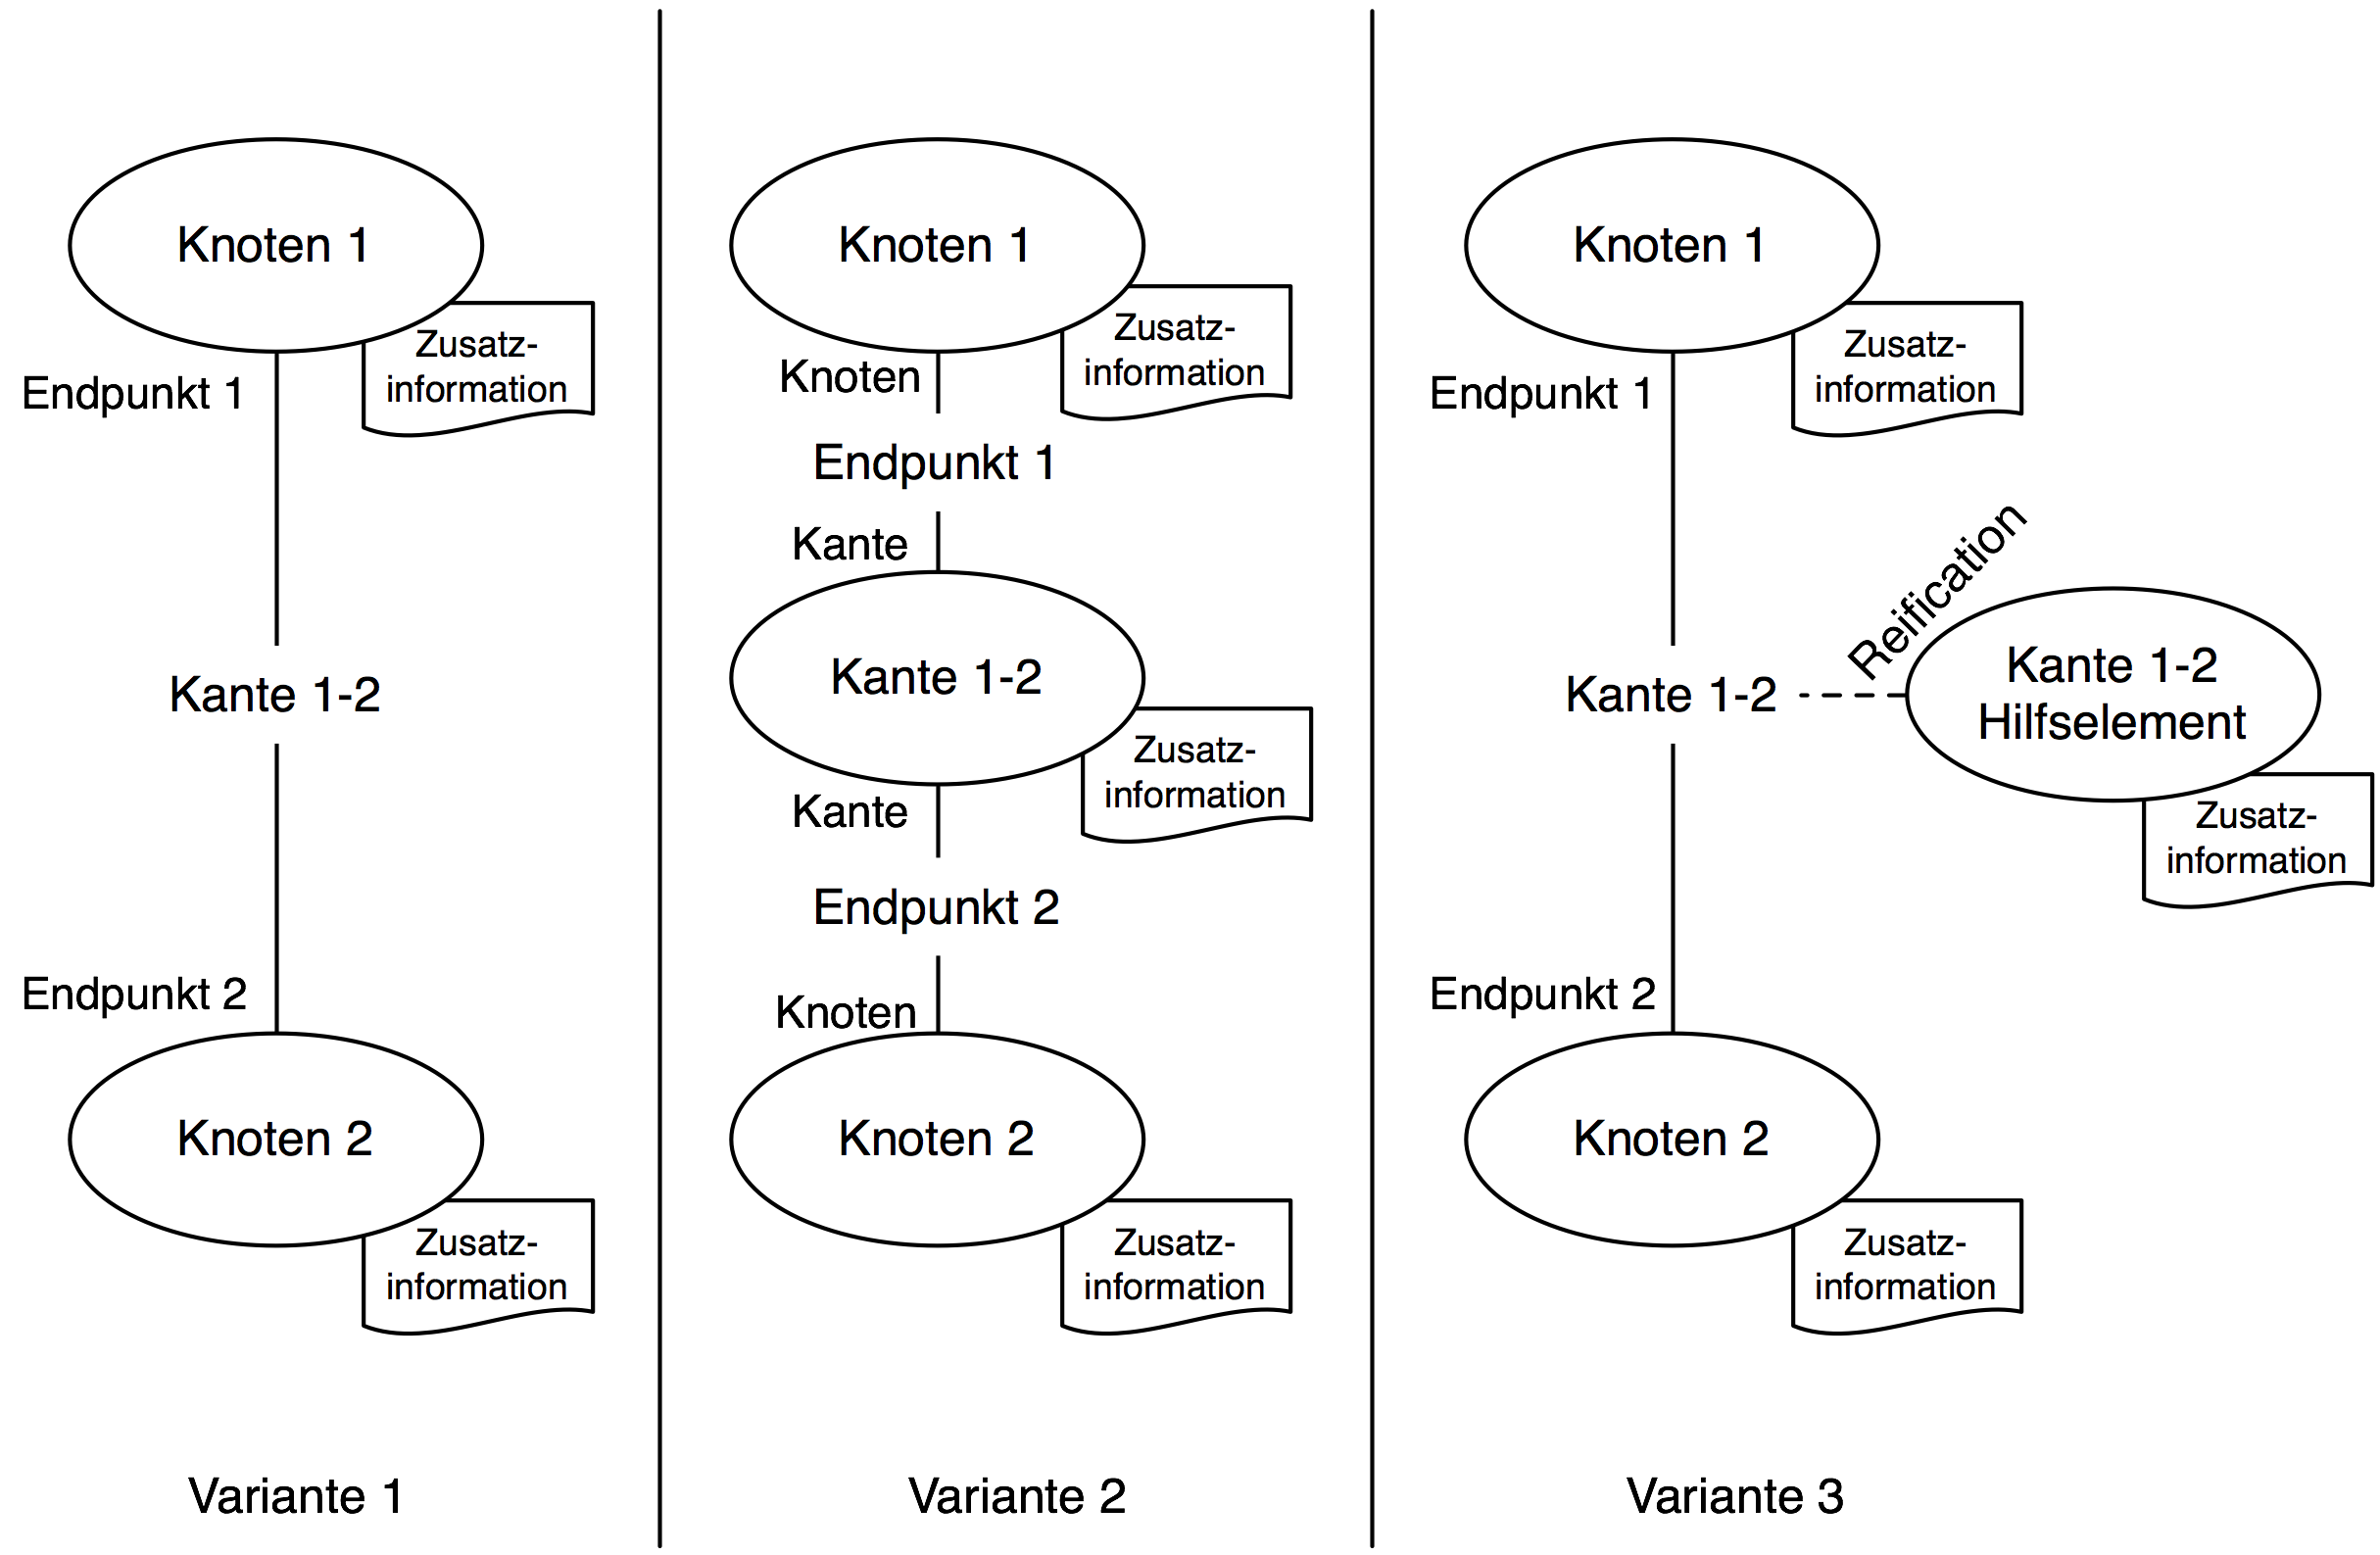
\includegraphics[width=13cm]{img/Persistenz/AssociationReification.png}
	\caption{Abbildung von Modellinformation in Topic Maps}
	\label{fig:img_Persistenz_AssociationReification}
\end{figure}

Die Bedeutung der Knoten des abzubildenden Modells im Kontext einer bestimmten Kante muss in den direkt abbildenden Varianten (in denen Kanten auf Associations abgebildet werden) durch Roles dargestellt werden. In der indirekten Abbildung (bei der Kanten auf Topics abgebildet werden), kann diese Information auch in den Associations repräsentiert werden, die die Topics die Knoten darstellen und jene die Kanten darstellen miteinander verbinden.
% subsection grundlegende_abbildung (end)

\subsection{Abbildung des Metamodells}
\label{sub:abbildung_des_metamodells}
Da Topic Maps von vorne herein nicht auf eine bestimmte semantische Bedeutung der Topics und Associations festgelegt sind, muss auch das Meta-Model der abgebildeten Modellierungssprache mit eingebettet werden. Dies wird in Topic Maps durch die Einbindung von Types ermöglicht. In den nun folgenden Ausführungen wird nur noch auf die direkt abbildende Variante Bezug genommen, da deren Ausdrucksstärke durch die Möglichkeit zur Reification gegenüber dem indirekt abbildenden Ansatz nicht eingeschränkt ist und die unmittelbare Abbildung zu insgesamt kleineren, einfacher zu verwaltenden Topic Maps führt (für eine Kanten wird nur eine Association benötigt, im Gegensatz dazu benötigt der alternative Ansatz ein Topic und mindestens zwei Associations zu Abbildung einer Kante).

Die in der Modellierungssprache festgelegten Arten von Knotentypen (also den eigentlichen Modellierungselementen) werden auf Topic Types abgebildet. Durch die Referenzierung eines einen Knoten repräsentierenden Topics auf diesen Topic Type wird die Bedeutung zugewiesen.

Ebenso wird mit Kanten verfahren. Durch die Einführung von Topics die als Association Types und Role Types fungieren, kann die Bedeutung einer Kante im abzubildenden Modell definiert werden. Dazu wird ein Association Type festgelegt, der die eigentliche Bedeutung der Kante festlegt, die zugehörigen Role Types definieren, wie viele Endpunkte existieren und welche Bedeutung diese haben. Für eine konkrete Kante wird dann eine Association und eine der Anzahl der Endpunkte entsprechende Nummer an Roles erstellt, denen der jeweilige Association bzw. Role Type zugewiesen wird. 

Die Verwendung von Occurrences und dementsprechend die Erstellung von Occurrence Types ist zur reinen Abbildung von diagrammatischen Modellen nicht notwendig. Die Verwendung von Occurrences kann aber sinnvoll sein, wenn aus dem ursprünglichen Modell ebenfalls Ressourcen referenziert werden, die für die weitere Verarbeitung des Modells notwendig sind. Occurrences werden dann im Sinne der Topic Map zur Referenzierung dieser Ressourcen verwendet, wobei sich die zu verwendenden Occurrence Types an der Bedeutung der Ressourcen im abzubildenden Modell orientiert.

Wie in Abschnitt \ref{sub:metamodellierung_in_topic_maps} bereits beschrieben, bietet die Topic Map selbst jedoch keine Möglichkeit, eine explizite Zuordnung zwischen Topic Types, Association Types und Role Types zu definieren, so dass ein in einer Topic Map repräsentiertes Modell auf semantische Korrektheit hin überprüft werden kann. Die einzige ohne zusätzliche Information überprüfbaren Bedingungen sind die Prüfungen, ob alle Knoten und Kanten (also Topics, Associations und Roles) einer Kategorie (also einem Type) zugewiesen  wurden.

Zusätzlich muss also eine externe Möglichkeit geschaffen werden, semantische Korrektheits-Bedingungen zu formulieren und zu überprüfen:
\begin{enumerate}
 \item Zulässige Kategorien von Knoten (Topic Types)
 \item Zulässige Kategorien von Kanten (Association Types, Role Types und eine Zuordnung zwischen diesen, die eine Aussage über die Anzahl und Bedeutung der Endpunkte der Kante zulässt)
 \item Zulässige Verbindungen zwischen Knoten und Kanten (Zuordnung zwischen Endpunkten einer Kantenkategorie und den Knotenkategorien, die diese Endpunkte belegen dürfen -- also eine Zuordnung zwischen Role Types und Topic Types)
\end{enumerate}

Wie bereits oben beschrieben, können derartige Bedingungen innerhalb oder außerhalb der Topic Map formuliert werden. Die Interpretation der formulierten Bedingungen und deren Anwendung auf konkrete Anwendungsfälle muss immer von außerhalb der Topic Map durchgeführt werden. Hier wird der Ansatz der Repräsentation der Bedingungen innerhalb der Topic Map verfolgt, um durch die Übermittlung einer Topic Map nicht nur ein Modell an sich zu übertragen sondern auch jene Information zu liefern, die zur Interpretation derselben notwendig ist.

Die Formulierung der Bedingungen erfolgt auf Ebene der als Types eingesetzten Topics und vervollständigt so das in der Topic Map enthaltene Meta-Modell der Sprache in der das zu repräsentierende Modell erstellt wurde. Die Information über zulässige Knoten und Kanten wird über die Festlegung von entsprechenden Types definiert. Für jeden Typen wird ein Topic eingeführt, das aus dem auf die Topic Map abgebildeten Modell referenziert werden kann. Alle oben notwendigen Zuordnungen zwischen diesen Types werden über Associations abgebildet, die die als Types verwendeten Topics verbinden (siehe Abbildung \ref{fig:img_Persistenz_MetaModelDef}).

\begin{figure}[htbp]
	\centering
		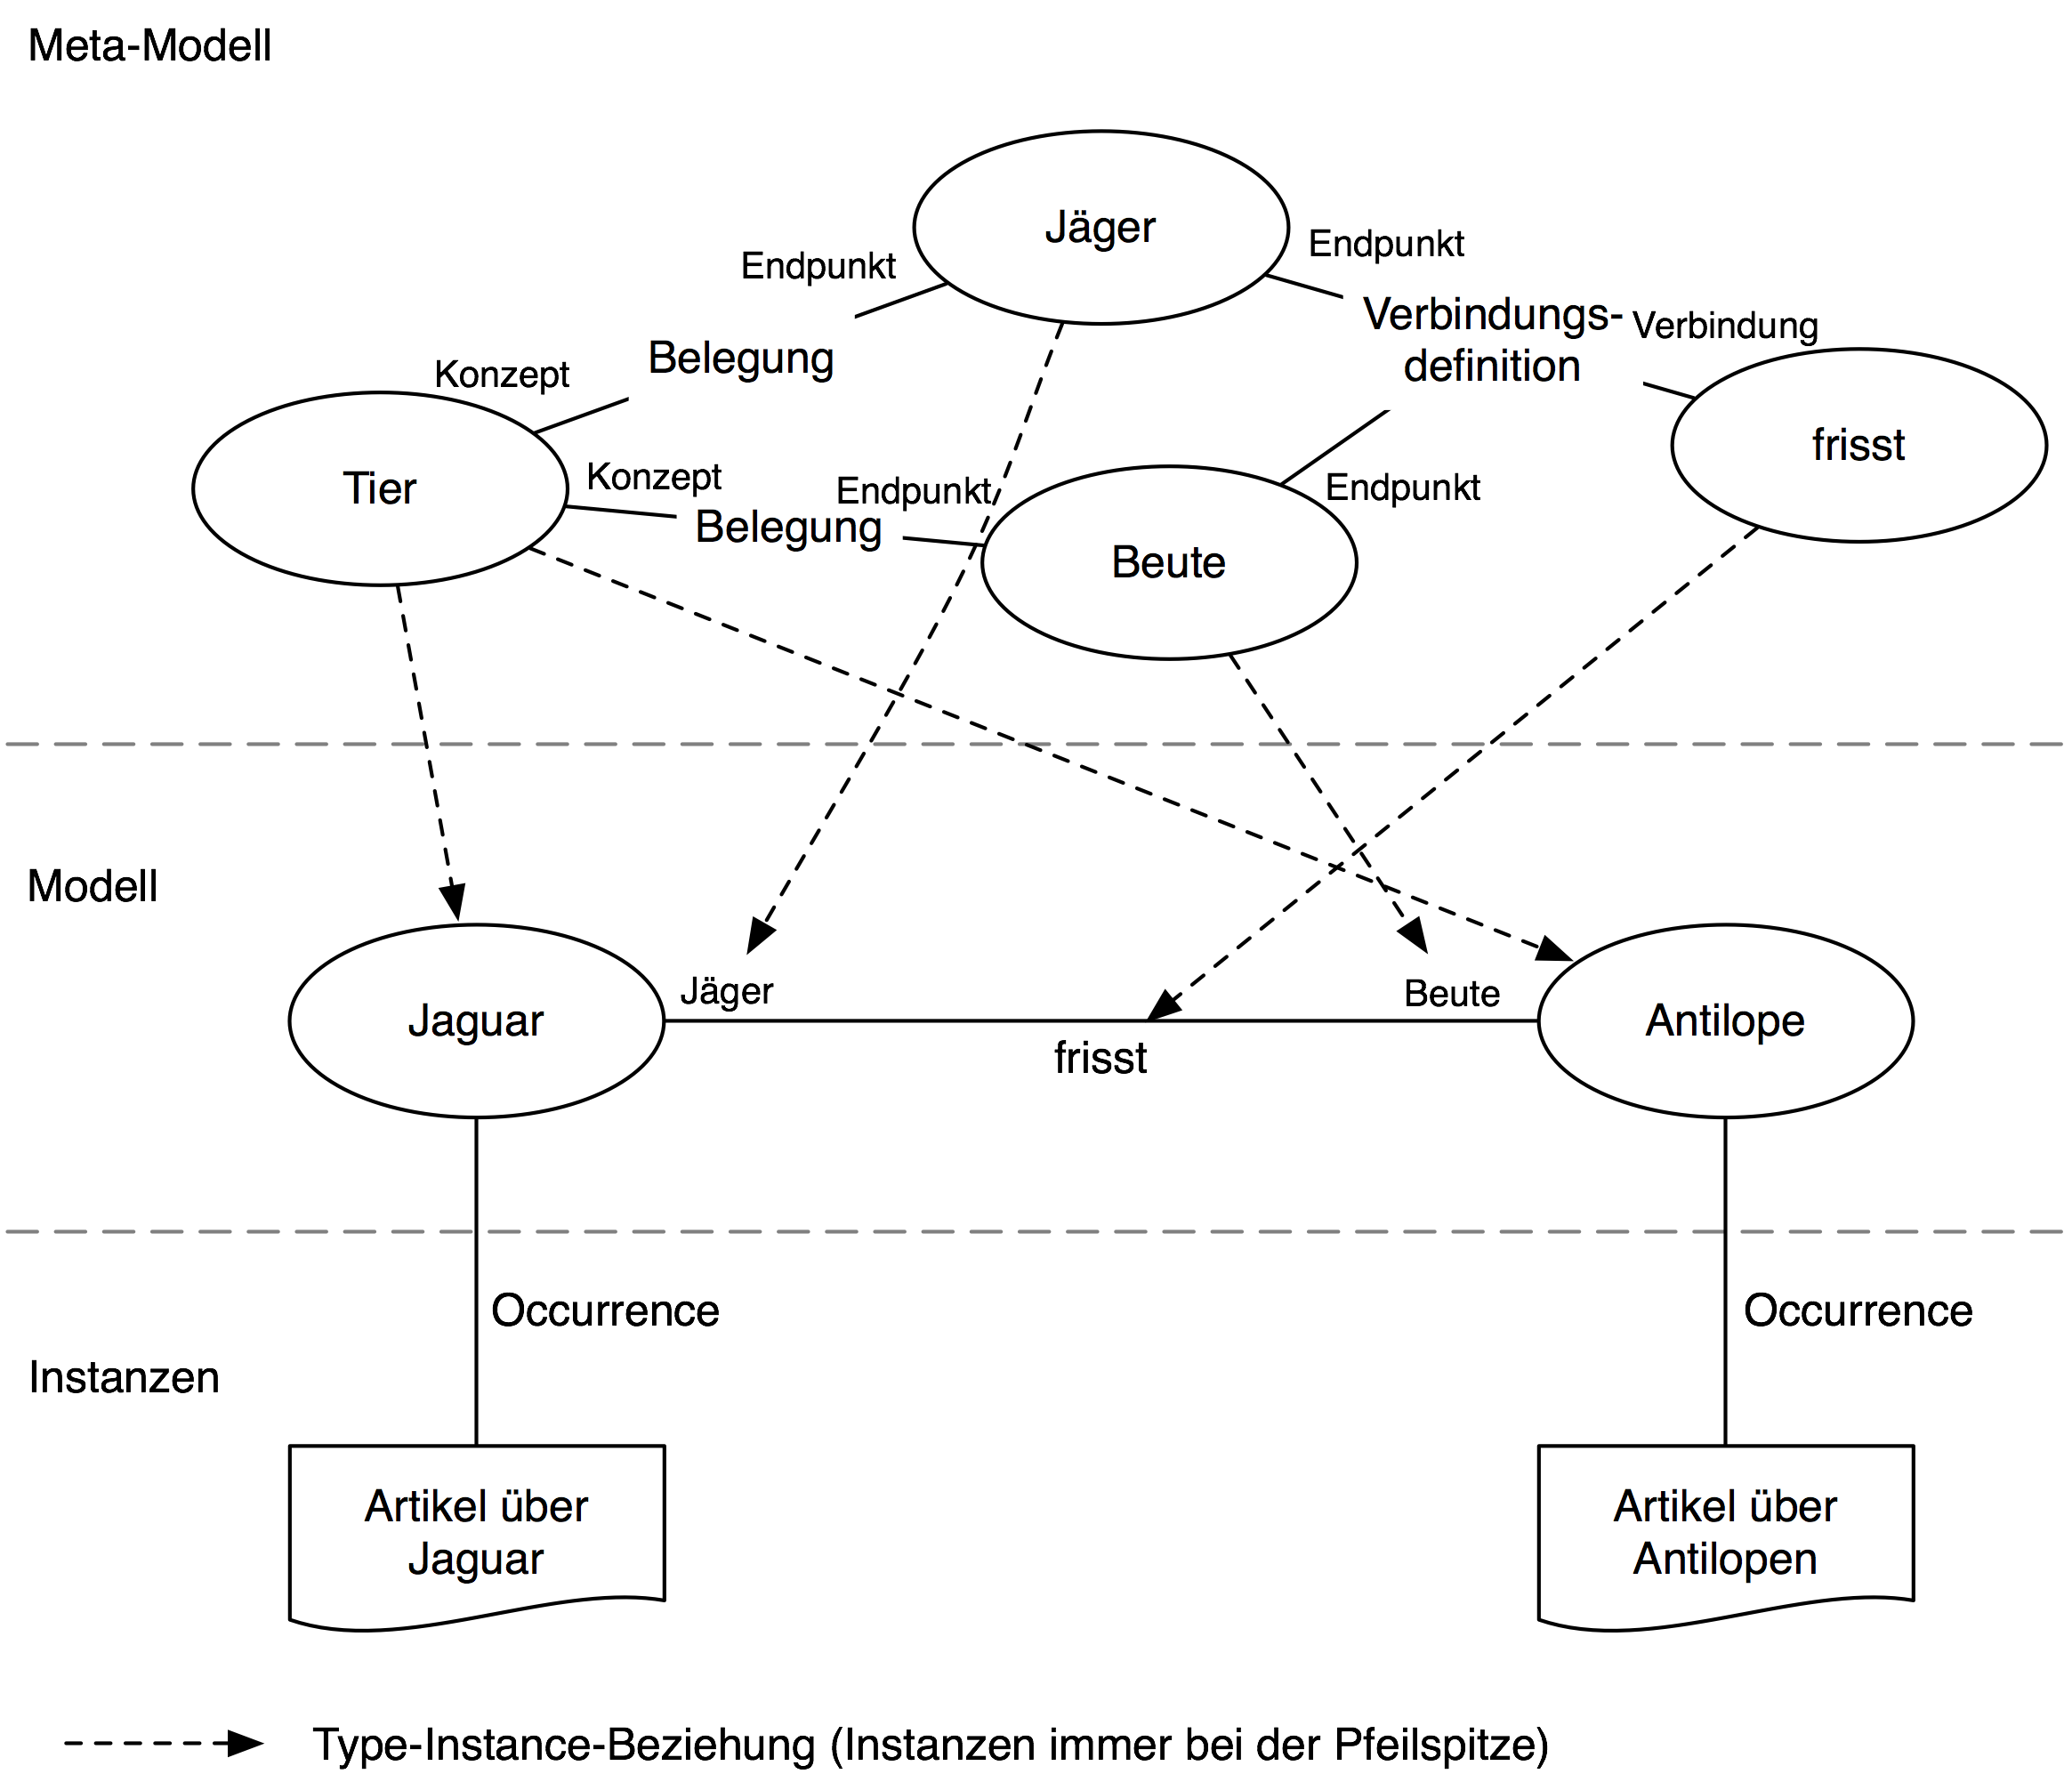
\includegraphics[width=13cm]{img/Persistenz/MetaModelDef.png}
	\caption{Definition des Meta-Models (ohne Kardinalitäten)}
	\label{fig:img_Persistenz_MetaModelDef}
\end{figure}

Die Definition der Kantentypen erfolgt über eine Association mit mindestens drei Roles. 
Eine dieser Roles referenziert den Association Type, die anderen Roles verweisen auf die zu verwendenden Role Types, die zur Beschreibung der Endpunkte der Kante verwendet werden (wovon mindestens zwei vorhanden sein müssen). Die Angabe der Kardinaliät (d.h. wie oft ein bestimmter Endpunkt im konkreten Modell auftreten darf) wird durch eine die jeweilige Role reifizierendes Topic festgelegt.

Ähnlich wird die Zuordnung zwischen Endpunkten und Knotenkategorien realisiert. Zwischen den entsprechenden Topic Types und Role Types werden Associations erstellt, die festlegen, ob eine bestimmte Knotenkategorie einen Endpunkt einnehmen darf oder nicht. Dazu enthält die betreffende Association mindestens zwei Roles, von denen eine auf den Role Type verweist, der den Endpunkt realisiert und eine entsprechende Anzahl von Roles, an die die zulässigen Topic Types (also Knotenkategorien) angebunden werden.

Die eben beschriebenen Abbildungsvorschriften selbst werden ebenfalls in der Topic Map abgebildet. Die Topic Map enthält damit auch das Meta-Meta-Modell das die Elemente die zur Festlegung eines Meta-Models und deren Zusammenspiel festlegt. Eine so definierte Topic Map ist also semantisch vollständig definiert und ermöglicht eine Rekonstruktion eines Modells, das in einer im Vorfeld unbekannten Sprache modelliert wurde, sofern lediglich das Meta-Meta-Modell bekannt ist, dass zur Interpretation der Sprachbeschreibung (Meta-Modell) notwendig ist (siehe Abbildung \ref{fig:img_Persistenz_MetaMetaModelDef}).

\begin{figure}[htbp]
	\centering
		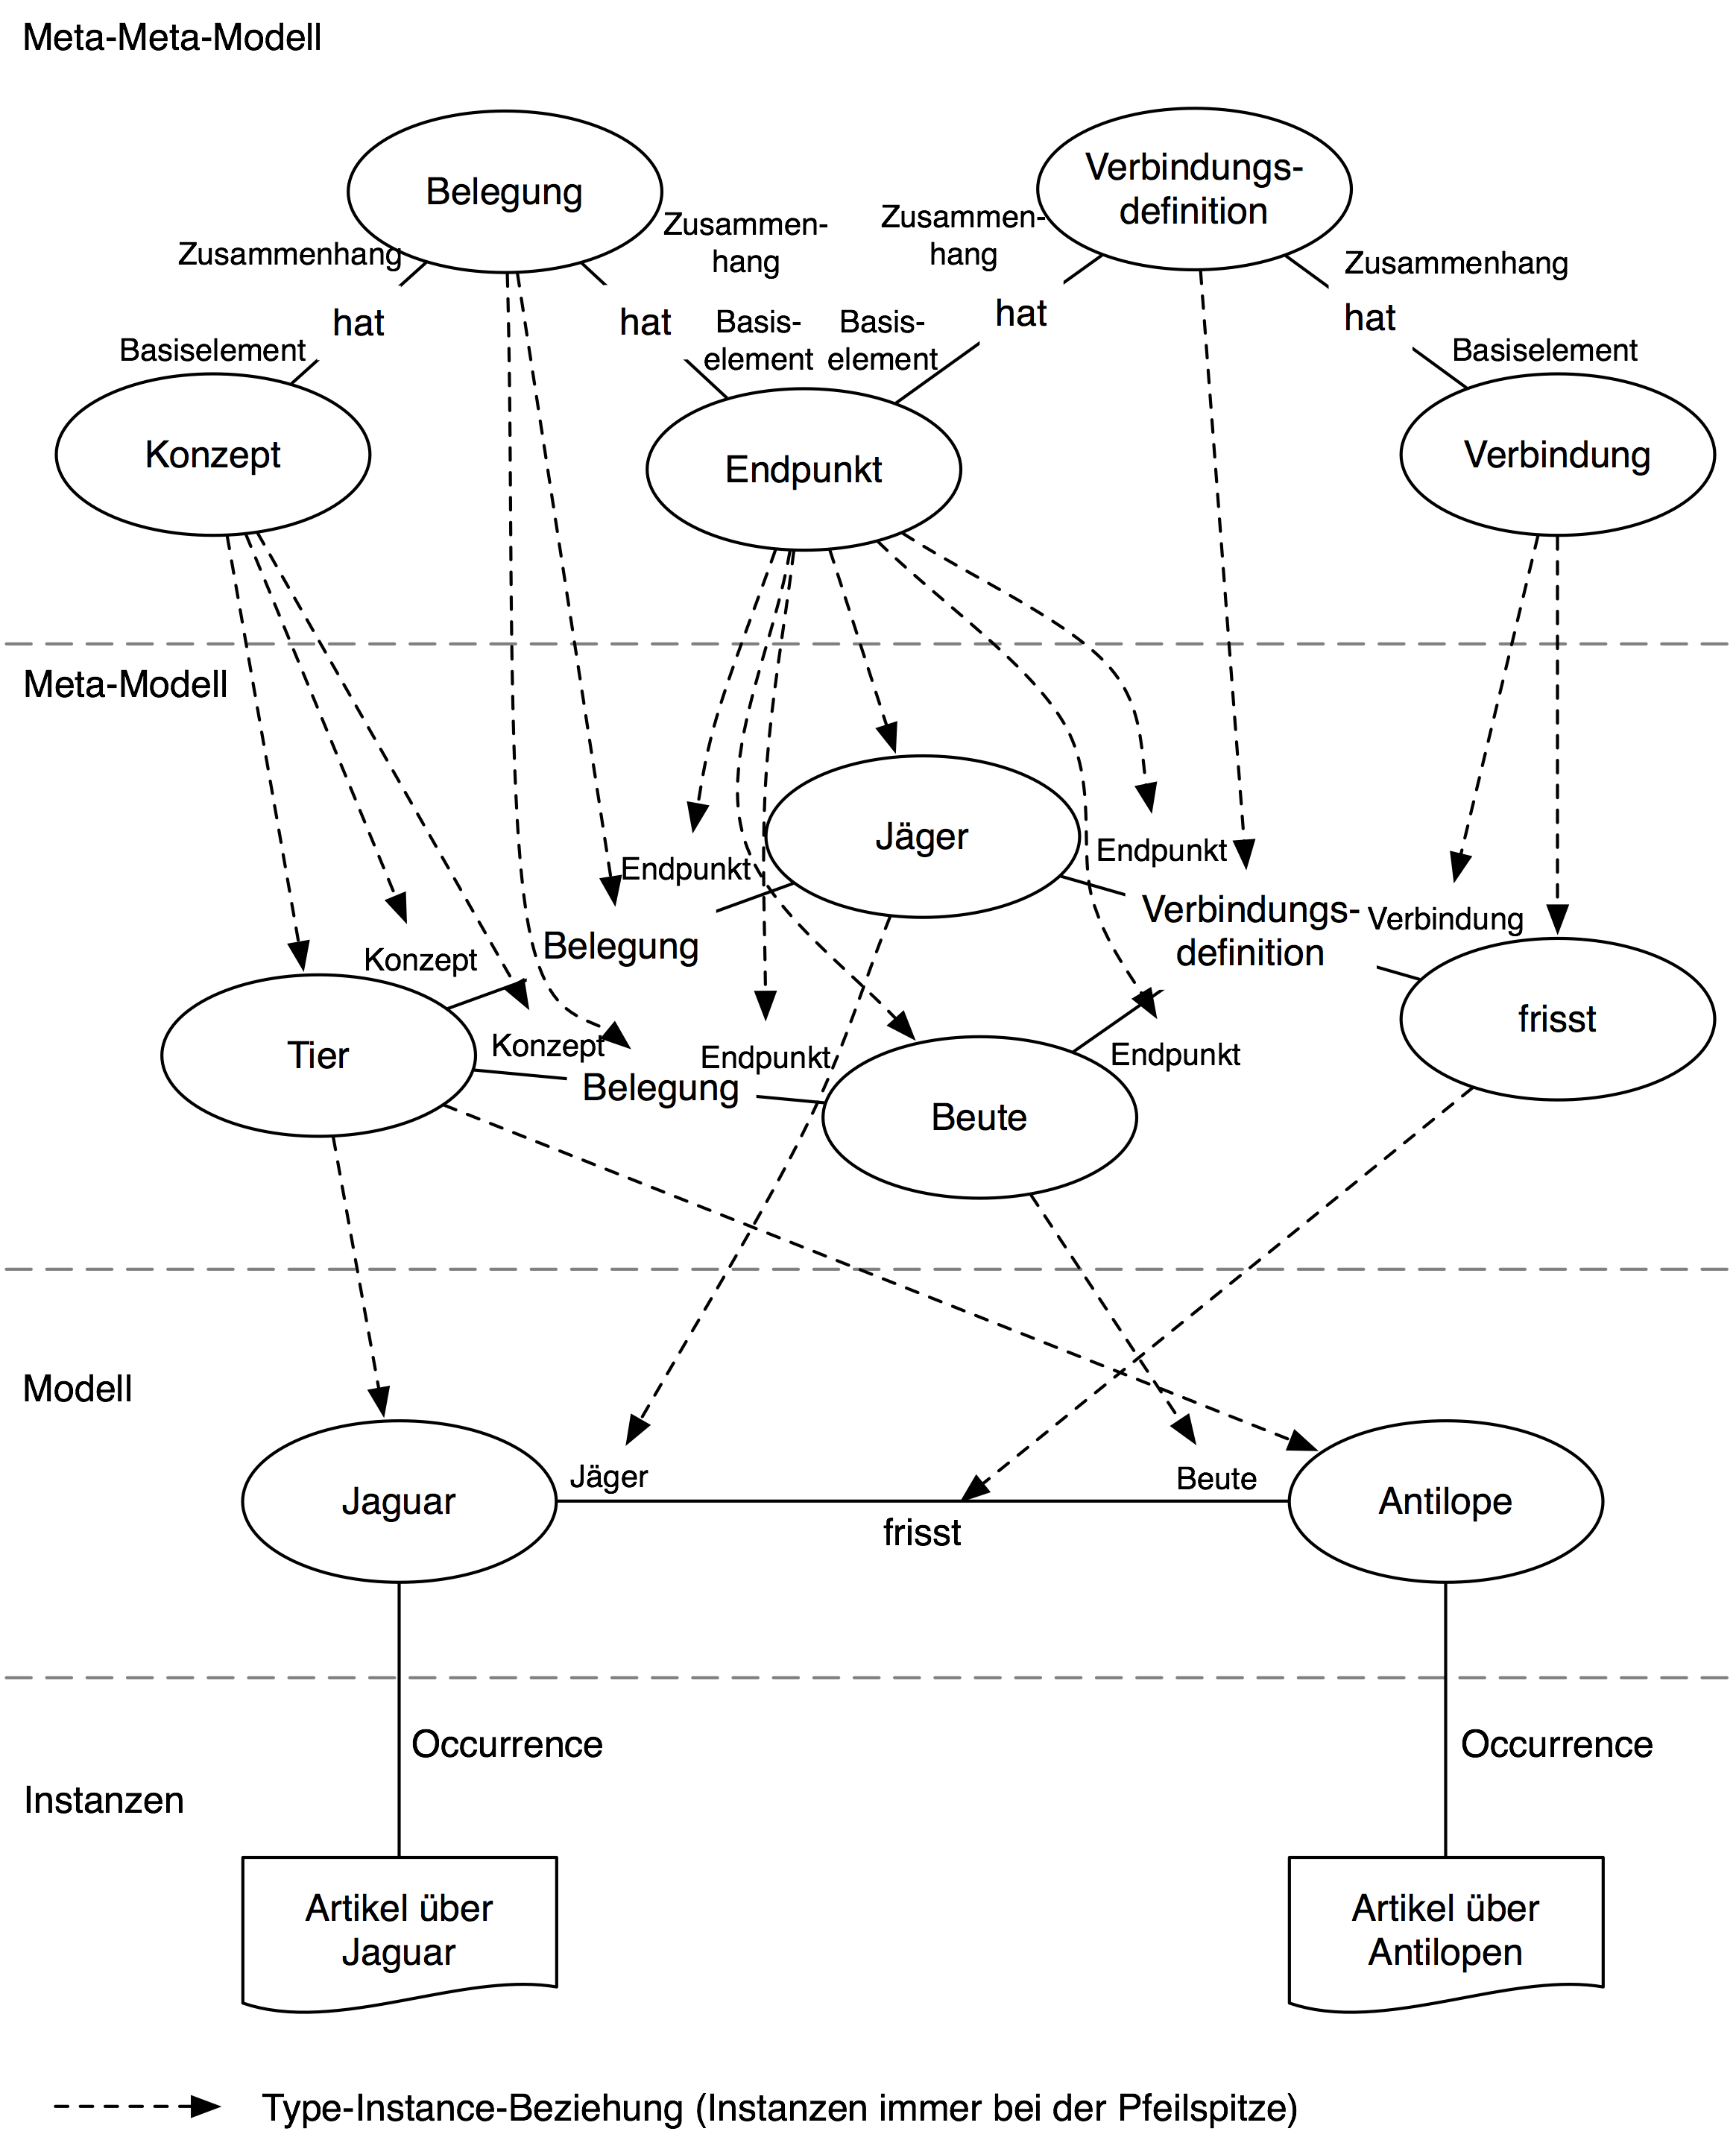
\includegraphics[width=13cm]{img/Persistenz/MetaMetaModelDef.png}
	\caption{Einbindung des Meta-Meta-Modells}
	\label{fig:img_Persistenz_MetaMetaModelDef}
\end{figure}

% subsection abbildung_des_metamodells (end)

\subsection{Abgrenzung von Submodellen}
\label{sub:abgrenzung_von_submodellen}

In einem Modell kann es sinnvoll oder notwendig sein, unterschiedliche Modellbereiche voneinander abzugrenzen. Der Grund für die Abgrenzung kann ein inhaltlicher sein (z.B. eine Partitionierung nach Akteuren bei Aktivitätsdiagrammen \citep{Rumbaugh04}) oder aus dem Modellierungsvorgang heraus motiviert sein (etwa bei der Abgrenzung von Teilmodellen, die durch verschiedene Personen erstellt wurden). Außerdem ist es möglich, in einer Topic Map mehrere Modelle zu repräsentieren, die ebenfalls voneinander abgrenzt werden müssen.

Für diese Abgrenzung bietet sich die Verwendung von Scopes an. Scopes haben zwar keinen Einfluss auf die vorhandenen Topics, wirken jedoch auf die Statements und -- hier relevant -- vor allem auf die die Topics verbindenden Associations. Werden also Scopes eingesetzt, um Teilmodelle voneinander zu unterscheiden bzw. zu trennen, so können die im Moment nicht relevanten Teilmodelle zwar nicht „ausgeblendet“ werden (im Sinne von „temporär vollkommen entfernt“, durch die Entfernung der nicht relevanten Statements sind jedoch nur noch jene Topics untereinander verbunden, die dem aktuell betrachteten Submodell angehören. Ausgehend von einer beliebigen, im Scope gültigen Association oder einem Topic, das bekannterweise dem aktuellen Teilmodell angehört kann so der gesamte relevante Teil der Topic Map erschlossen werden.

Die Realisierung der Trennung zwischen Teilmodellen durch das Ausblenden irrelevanter Verbindungen zwischen Topics birgt einen weiteren potentiellen Vorteil. Werden in einer Topic Map mehrere untereinander zusammenhängende Modelle abgebildet, so wird -- der Grundforderung einer Topic Map nach Eineindeutigkeit entsprechend -- jedes Element nur einmal abgebildet, egal ob es in nur einem Modell verwendet wird oder in mehreren. Durch den Einsatz von Scopes bilden in mehreren Modellen verwendete Elemente automatisch eine Schnittstelle, an der zwischen den Modellen navigiert werden kann. Dieser Vorteil muss in herkömmlichen Modellierungsansätzen mit mehreren untereinander verknüpften Modellen wie der \gls{UML} \citep{Rumbaugh04} oder ARIS \citep{Scheer03} technisch durch explizite Verknüpfung bzw. Referenzierung der äquivalenten Modellelemente in den unterschiedlichen Modeller erzeugt werden. 

Zur Kennzeichnung des Scopes muss zumindest ein Topic verwendet werden. Im Meta-Modell muss festgelegt werden, ob dazu ein Topic eines bestehenden Types verwendet wird oder ein neuer Type eingeführt werden, dessen Topics ausschließlich zum Aufspannen eines Scopes verwendet werden. Dazu wird im Meta-Meta-Modell ein Type „Partition“ eingeführt, der der für alle Elemente des Meta-Modells verwendet werden muss, deren konkrete Instanzen einen Scope im Modell kennzeichnen sollen.

% subsection abgrenzung_von_submodellen}

\subsection{Flexibilisierung der Abbildung}
\label{sub:flexibilisierung_der_abbildung}

Wie in Kapitel XY beschrieben, ist das Meta-Modell von Modellen die im vorgestellten Ansatz entstehen, nicht im vorhinein festgelegt. Die Modellierungssprache -- also das Meta-Modell -- wird während der Modellbildung semantisch definiert und ist damit erst zur Modellierungszeit bekannt. Das Metamodell kann außerdem während der Modellierung erweitert werden, es ist auch möglich, dass sich die Bedeutung bereits existierender Meta-Modell-Elemente ändert.

Für die Persistierung bedeutet dies, dass das Meta-Modell nicht im Vorhinein sondern erst zum Zeitpunkt der Speicherung festgeschrieben werden kann. Außerdem kann die Prüfung auf semantische Korrektheit des Modells ebenfalls nur durchgeführt werden, sobald das Modell definiert ist. 

Um die geforderte Flexibilität bei der Sprachdefinition in Form und Zeitpunkt zu gewährleisten, wurde von \citet{Neubauer08} ein System entwickelt, dass es erlaubt, dynamisch zur Laufzeit Modellelemente zu definieren, die Regeln zu deren Verwendung festzulegen und diese ohne Unterbrechung des Modellierungsvorgangs unmittelbar zu verwenden (wobei auch die Prüfung der semantischen Korrektheit zur Laufzeit adaptiert wird). Die technische Umsetzung dieses Ansatzes wird in Abschnitt \ref{sec:dynamische_metamodelle} beschrieben.

% subsection flexibilisierung_der_abbildung (end)

% section abbildung_von_modellen_auf_topic_maps (end)

\section{Technische Umsetzung der Persistierung von Modellen} % (fold)
\label{sec:technische_umsetzung_der_persistierung_von_modellen}

Die oben beschriebenen Konzepte zur Persisitierung von Modellen wurden wie die übrigen Software-Komponenten des Systems in Java implementiert. Die Basis der Persistenz-Komponente bildet eine Topic Map Engine, die im Rahmen einer Arbeit über flexible Content-Repräsentation vom Autor entwickelt wurde \citep{Oppl07}. Das in \citep{Neubauer08} entwickelte System zur Generierung und Verwendung dynamischer Metamodelle, das bereits in Abschnitt \ref{sub:flexibilisierung_der_abbildung} konzeptuell beschrieben wurde, wird in der Folge hinsichtlich seiner technischen Umsetzung betrachtet. Basierend auf diesen beiden Komponenten wurde die eigentlichen Persistierung implementiert. Der dort verfolgte Ansatz ist Thema des letzten Teils dieses Abschnitts.

\subsection{Topic Map Engine}
Topic Map Engine Persistence Layer

\subsection{Dynamische Metamodelle}
\label{sec:dynamische_metamodelle}

\subsection{Persistierung}
% section technische_umsetzung_der_persistierung_von_modellen (end)


\section{Export graphischer Repräsentationen} % (fold)
\label{sec:export_graphischer_repräsentationen}

Neben der Persistierung der Modelle in Form einer Topic Map ist es auch sinnvoll, die Modelle in deren graphischer Form als Referenz abzulegen. Das hier entwickelte Werkzeug bedient sich der graphischen Ausgabefunktionalitäten, die der Java Klassenbibliothek mit der Version 1.4 hinzugefügt wurden, um das aktuelle Modell in unterschiedlichen Formen als Grafik auszugeben und zur späteren Referenz zu speichern.

\subsection{Ausgabeformen} % (fold)
\label{sub:ausgabeformen}

Zur Speicherung der graphischen Repräsentation eines Modells wird grundsätzlich die Visualisierung verwendet, die auf dem sekundären Ausgabekanal (also dem Bildschirm) zur Anwendung kommt. Beim Export sind nun unterschiedliche Modellaspekte zu berücksichtigen, die je nach intendiertem Verwendungszweck einzeln oder in Kombination in die Ausgabe eingehen können. Diese Aspekte sind im Einzelnen
\begin{itemize}
	\item der aktuell auf der Oberfläche befindliche Modellzustand
	\item die hierarchisch in diesen eingebetteten Submodelle
	\item die Modellierungshistorie, also die Entwicklung des Modells über die Zeit
\end{itemize}

Die Darstellung dieser Aspekte in einer graphischen Repräsentation ist (außer im erstgenannten Fall) insofern komplex, als dass eine beliebig lange zeitliche Abfolge bzw. eine beliebig tief verschachtelte Hierarchie in den zweidimensionalen Raum abgebildet werden muss. Im Falle einer Kombination des zweit- und drittgenannten Aspektes müssen zwei Dimensionen zugleich abgebildet werden, was die Darstellung zusätzlich erschwert.

Der aktuell auf der Oberfläche befindliche Modellzustand wird exakt wie dargestellt in eine Grafik transformiert und als Bild abgespeichert. Zur Abbildung der Modellierungshistorie bietet sich an, die einzelnen gespeicherten Modellzustände chronologisch anzuordnen. Der sich so ergebende Zeitstrahl beginnt links oben und setzt sich von links nach recht und oben nach unten bis in die rechte untere Ecke fort, wo wiederum der aktuelle Modellzustand dargestellt wird. Die zweidimensionale Abbildung des Zeitstrahls erfolgt dabei derart, das sowohl die horizontale als auch die vertikale Ausdehnung des resultierenden Bildes minimal sind (siehe Abbildung \ref{fig:img_Persistenz_ExportHistorie}).

\begin{figure}[htbp]
	\centering
		\includegraphics[width=15cm]{img/Persistenz/ExportHistorie.png}
	\caption{Modellierungshistorie als exportierte Grafik}
	\label{fig:img_Persistenz_ExportHistorie}
\end{figure}

Bei der Darstellung eines Modells mit hierarchisch geschachtelten Teilmodellen bietet sich eine baumartige Darstellung mit dem aktuellen Modellzustand als Wurzelknoten an. Diese ist aufgrund der notwendigen Detaildarstellung der einzelenen Modelle jedoch platzintensiv und kann nur schwer als physisches Dokument abgelegt werden. Deshalb wurde alternativ die hierarchische Strukur auf eine der Darstellung der zeitlichen Modellentwicklung ähnliche Darstellungsform abgebildet. Dabei wird die Hierarchie flach ausgerollt, die Einbettungen zeigen sich durch einen graduell dunkler werdenden Modellhintergrund für tiefere verschachtelte Ebenen. Zusätzlich wird in jedes Submodell farblich abgesetzt auch das jeweilige Containerelement eingeblendet. Die Abfolge der einzelnen Modelle startet mit dem aktuellen Modellzustand als erstem Knoten. Dahinter wird das erste im aktuellen Modell eingebettete Teilmodell angezeigt. Besitzt dieses Teilmodell wiederum eingebettete Teilmodelle, so werden diese in der Folge mit erneut abgedunkeltem Hintergrund dargestellt. Diese Form der Darstellung wird fortgesetztm bis keine weiteren eingebetteten Modelle mehr vorhanden sind. Es folgt (sofern vorhanden) das zweite Submodelle des aktuellen Modellzustandes (mit dem abgedunkelten Hintergrund der ersten Einbettungsebene). Diese Hierarchie wird wiederum bis zu den Endpunkten nach unten verfolgt, es folgt ggf. das dritte Submodell auf der ersten Einbettungsebene. Die sich so ergebende Linie an Modellzuständen wird wie der chronologischen Darstellung der Modellierungshistorie so umgebrochen dass sich sowohl in horizontaler als auch in vertikaler Richtung eine minimale Ausdehung ergibt (siehe Abbildung \ref{fig:img_Persistenz_ExportHierarchie}).

\begin{figure}[htbp]
	\centering
		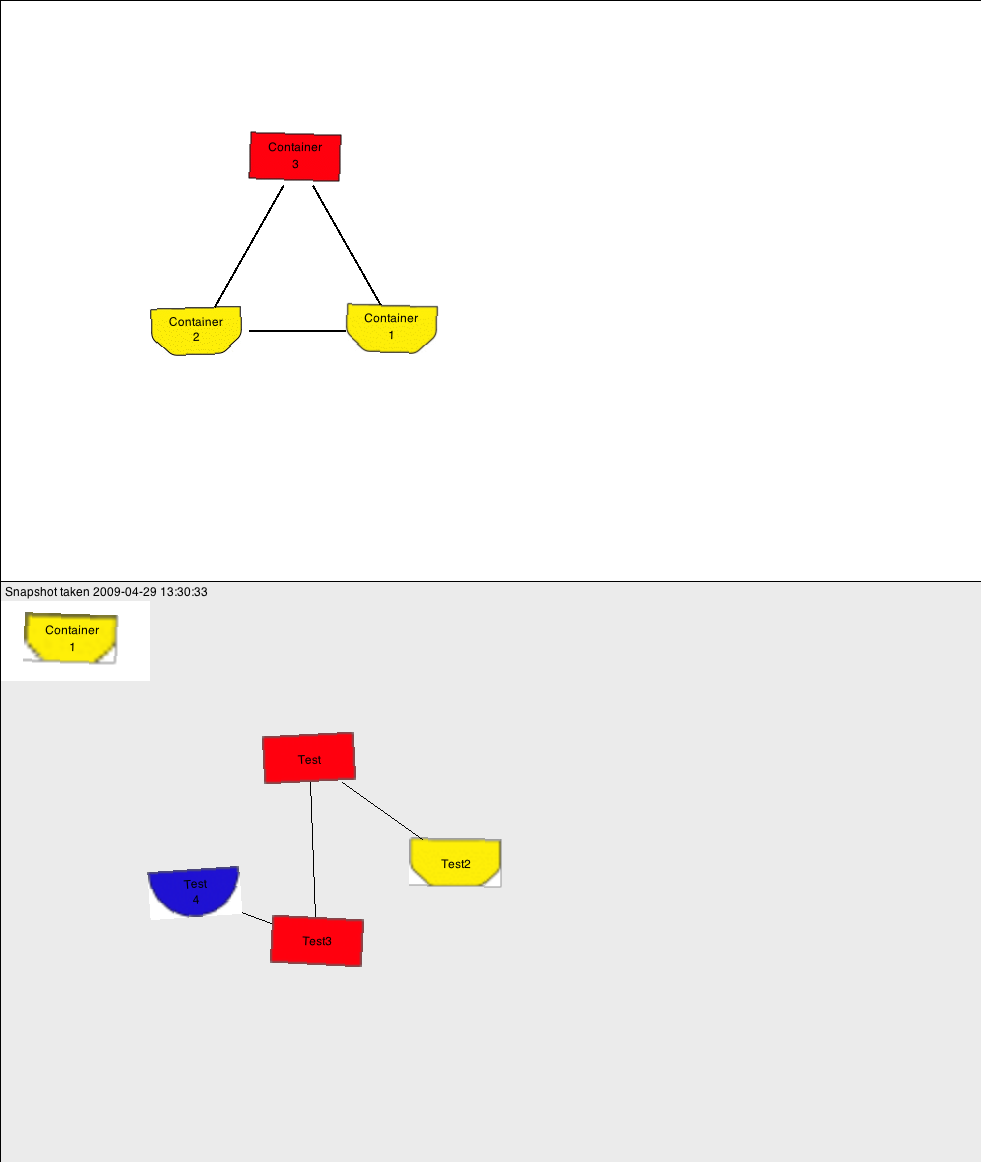
\includegraphics[width=15cm]{img/Persistenz/ExportHierarchie.png}
	\caption{Modell-Hierarchie als exportierte Grafik}
	\label{fig:img_Persistenz_ExportHierarchie}
\end{figure}

In der komplexesten Ausprägung der Darstellung eines Modells als graphische Repräsentation werden sowohl die Historie der Modellentstehung als auch die Hierarchie der eingebetteten Submodelle zugleich dargestellt. Dies erfolgt hier durch die Kombination der beiden eben beschriebenen Ansätze. Die Darstellung der Modellierungshistorie bildet die oberste Ebene der Modelldarstellung. Beginnend mit dem ältesten gespeicherten Modellzustand werden die einzelnen Modelle in der Reihenfolge ihrer Entstehung abgebildet, wobei zu jedem Modellzustand unmittelbar folgend dessen eingebetteten Submodelle ausgegeben werden (deren Entstehung nicht mehr separat dargestellt wird). So ergibt sich eine kombinierte Linie aus chronologischer Modellentwicklung und eingebetteten Teilmodellen. Diese wird wie schon oben mit minimaler Ausdehnung in horizontaler wie vertikaler Richtung auf eine Grafik abgebildet. Die Entwicklung des Modells ist dabei wie gehabt von links oben nach rechts unten zu verfolgen, wobei nur jene Modellzustände mit weißem Hintergrund auf oberster Ebene der Zeitlinie angehören. Alle dunkler hinterlegten Modelle sind Teilmodelle und sind dem nach vorne nächstgelegenen weiß hinterlegten Modell zuzuordnen.

% subsection ausgabeformen (end)

\subsection{Technische Umsetzung des graphischen Exports} % (fold)
\label{sub:technische_umsetzung_des_graphischen_exports}

Zur Umsetzung des graphischen Exports wird auf die mit der Java Plattform in der Version 1.4 eingeführten Klassen zu Verarbeitung von Grafikformaen zurückgegriffen. Diese unterstützen standardmäßig gängige Grafikformate wie \gls{JPEG}, \gls{GIF} oder \gls{PNG}. Im konkreten Fall wurde ein verlustfrei komprimierendes Format gewählt, verlustbehaftete Verfahren wie \gls{JPEG} sind für die hier abzubildenden feinen Strukturen nicht geeignet, da es durch Kompressionsartefakte zu Qualitätsminderungen in der Darstellung von Details kommt.

Die Ausgabe einer Datei im gewählten Grafikformat wird vollständig von der Klasse \texttt{ImageIO} übernommen. Der Schnittstellen-Methode \texttt{write} sind als Parmeter der Dateiname, das Grafikformat sowie ein Objekt der Klasse \texttt{BufferedImage} (allgemeiner: einer Klasse, die das Interface \texttt{RenderedImage} implementiert) zu übergeben, dass die eigentlichen Bilddaten enthält.

Das \texttt{BufferedImage}-Objekt kann durch einen Methoden-Aufruf mit der graphischen Repräsentation einer Klasse, die von der Java \gls{AWT}-Klasse \texttt{Component} abgeleitet ist, befüllt werden. Da alle graphischen Komponenten des JHotDraw-Frameworks Subklassen eben dieser Klasse sind (inklusive der Zeichenoberfläche selbst), können diese durch einen Aufruf ihrer \texttt{paint}-Methode in ein ausreichend großes \texttt{BufferedImage} (bzw. dessen \texttt{Graphics}-Objekt) geschrieben werden.  

In den aus mehr als einem Teilmodell bestehenden Ausgaben (also der Historie, der hierarchischen Darstellung der Teilmodelle oder der Kombination dieser beiden Fälle) muss das Bild aus den graphischen Repräsentationen der einzelnen Teilmodelle zusammengesetzt werden. Dazu werden (im Falle der hierarchischen Teilmodelle rekursiv) die logischen Modelle erzeugt und bereits in der korrekten linearisierten Darstellungsform in einem \texttt{Vektor} gespeichert. Die einzelnen logischen Modelle werden dann in graphische Repräsentationen umgewandelt und in je einem \texttt{BufferedImage} gespeichert. Diese werden in der Folge so zusammengesetzt, dass die horizontale und vertikale Ausdehung der Gesamtfläche minimal ist.

% subsection technische_umsetzung_des_graphischen_exports (end)
% section export_graphischer_repräsentationen (end)

\section{Zusammenfassung} % (fold)
\label{sec:persistierung_zusammenfassung}

% section persisitierung_zusammenfassung (end)
% chapter persistierung (end)


% part umsetzung (end)

